%%%%%%%%%%%%%%%%%%%%%%%%%%%%%%%%%%%%%%%%%%%%%%%%%%%%%%%%%%%%%%%%%%%%%%%%%%%%%%%%
%                     Bachelor thesis template
%						 Science Faculty
%								at
%			National Autonomous University of Mexico (UNAM)
%%%%%%%%%%%%%%%%%%%%%%%%%%%%%%%%%%%%%%%%%%%%%%%%%%%%%%%%%%%%%%%%%%%%%%%%%%%%%%%%
% based on Harish Bhanderi's PhD/MPhil template, then Uni Cambridge
% http://www-h.eng.cam.ac.uk/help/tpl/textprocessing/ThesisStyle/
% corrected and extended in 2007 by Jakob Suckale, then MPI-iCBG PhD programme
% and made available through OpenWetWare.org - the free biology wiki
%
%                     Under GNU License v3
%
% Adapted for the Engineering School at UNAM by Jesús Velázquez y Marco Ruiz
% Then, adapter fot he Science Faculty at UNAM by Jonathan Urrutia
%
%
%
% All used packages are found in
%
%					./Latex/Classes/PhDthesisPSnPDF.cls
%
% within this last document, there are some lines to be UnCommented for a printed or a digital version of the output file:
%
%			line 184
%			lines 231-261hfill
%
%	Since this is a template for a thesis made at UNAM (Mexico) the titles may be in spanish but within PhDthesisPSnPDF.cls it can be change
%

\documentclass[11pt]{Latex/Classes/PhDthesisPSnPDF}

\usepackage{blindtext}         %  For dummy text.
% The \blindtext or \Blindtext commands throughout this template generate dummy text to fill the template out.

%--------------------Cambiar captio de las subfiguras -------------------
\renewcommand*{\thesubfigure}{\alph{subfigure})}   %Cambia caption y también el \ref{   }  

	\newcommand{\beqhalf}{\noindent \begin{minipage}[c]{.5\linewidth} \begin{equation}}
	\newcommand{\eeqhalf}{\end{equation} \end{minipage} }
	\newcommand{\eqhalf}[1]{\beqhalf #1 \eeqhalf}	


\usepackage{animate}  %pARA EL GIF



%\makeatletter
%\newenvironment{taggedsubequations}[1]
% {%
%  % \end{subequations} will advance `equation`
%  \addtocounter{equation}{-1}%
%  \begin{subequations}%
%  % set the current label
%  \def\@currentlabel{#1 \emph{bis}}%
%  % redefine \theequation
%  \renewcommand{\theequation}{#1\alph{equation} \emph{bis}}%
% }
% {\end{subequations}}
%\makeatother %not \makeatletter

\makeatletter
\newenvironment{taggedsubequations}[1]
 {%
  % \end{subequations} will advance `equation`
  \addtocounter{equation}{-1}%
  \begin{subequations}%
  % set the current label
  \def\@currentlabel{#1}%
  % redefine \theequation
  \renewcommand{\theequation}{#1\alph{equation}}%
 }
 {\end{subequations}}
\makeatother %not \makeatletter




%%% Local Variables:
%%% mode: latex
%%% TeX-master: "~/Documents/LaTeX/CUEDThesisPSnPDF/thesis"
%%% End:
           % Special commands written by the author


\svgpath{{1-Theory/figs},{5-Apendices/figs},{2-Results/figs}}
\graphicspath{{5-Apendices/figs},{0-5-Introduccion/figs}}
\lstset{basicstyle=\ttfamily\footnotesize,breaklines=true}


\usepackage{Latex/mmacells}
\usepackage{Latex/coffee4}
\usepackage{rotating}

\mmaDefineMathReplacement[≤]{<=}{\leq}
\mmaDefineMathReplacement[≥]{>=}{\geq}
\mmaDefineMathReplacement[≠]{!=}{\neq}
\mmaDefineMathReplacement[→]{->}{\to}[2]
\mmaDefineMathReplacement[⧴]{:>}{:\hspace{-.2em}\to}[2]
\mmaDefineMathReplacement{∉}{\notin}
\mmaDefineMathReplacement{∞}{\infty}
\mmaDefineMathReplacement{𝕕}{\mathbbm{d}}


\mmaSet{
  morefv={gobble=2},
  linklocaluri=mma/symbol/definition:#1,
  morecellgraphics={yoffset=1.9ex}
}
\allowdisplaybreaks
\DeclareMathAlphabet\mathbfcal{OMS}{cmsy}{b}{n}

%%-------------------------------------------------------------------------------
%                                  Information of the Student
%-------------------------------------------------------------------------------
% --- Default information for Bachelor's degree
%\author{Jonathan Alexis Urrutia Anguiano}
%\title{Optical response of partially embedded nanospheres}
%\programa{Posgrado en Ciencias Físicas} % Licenciatura en Física
%\degree{Maestro en Ciencias}% Maestro en / Doctor en
%\director{Dr. Alejandro Reyes Coronado}% Thesis director
%\facultad{Facultad de Ciencias}
%\lugar{Ciudad de México, México}% Place of the dissertation
%\degreedate{2021}% Year of the dissertation
%\portadatrue   %Uncomment for color cover

% ----------------------------- Datos del jurado de Licenciatura
%\student{Paternal last name\\ Maternal Last name\\ Names\\ Telephone number\\ Universidad Nacional Autónoma de México\\ Facultad de Ciencias\\ Física\\ Student Number}
%\secretario{Dr \\ Secretary (thesis director) \\ Last name \\ Last name}
%\presidente{Dr \\ President \\ Last name \\ Last name}
%\vocal{Dr \\ Vocal \\ Last name \\ Last name}
%\supuno{Dr \\ substitute 1 \\ Last name \\ Last name}
%\supdos{Dr \\ Substitute 2 \\ Last name \\ Last name}
%\pags{pages}


% --- Default information for Grad degree

\posgradotrue
	 \author{Jonathan Alexis Urrutia Anguiano}
		 \title{Optical response of partially embedded nanospheres}
		 \programa{Posgrado en Ciencias Físicas} 	% Programa de posgrado
		  \degree{Maestro en Ciencias}				% Maestro en / Doctor en

	\director{Dr. Alejandro Reyes Coronado}		% Thesis director
	\directordep{Facultad de Ciencias, UNAM}

	\lugar{Ciudad de México, México}			% Place of the dissertation
	\degreedate{2022} 							% Year of the dissertation  - Arreglar espacio inicial
	\campo{Física}								% Area del posgrado

	\comitetrue									% Comité académico en la portada
											% Falta ver si se ponen extra dentro del documento
		\ctutoruno{Dra. Citlali Sánchez-Aké}
		\ctutorunodep{Instituto de Ciencias Aplicadas y Tecnología, UNAM}
		\ctutordos{Dr. Giuseppe Pirruccio}
		\ctutordosdep{Instituto de Física, UNAM}

\keywords{tesis,autor,tutor,etc}            % For metadata
\subject{tema_1,tema_2}                     % Subjects for metadata














%-------------------------------------------------------------------------------
%                                   COVER
%-------------------------------------------------------------------------------
\begin{document}
%
\maketitle
%-------------------------------------------------------------------------------
%                                   FRONT MATTER
%-------------------------------------------------------------------------------
\frontmatter

% !TeX root = ../tesis.tex

\begin{acknowledgements}
\addcontentsline{toc}{chapter}{\protect\numberline{}Acknowledgements}



\blindtext 

\end{acknowledgements}





%% ******************************* Thesis Declaration ********************************

\begin{declaration}

Por la presente declaro que, salvo cuando se haga referencia específica al trabajo de otras personas, el contenido de esta tesis es original y no se ha presentado total o parcialmente para su consideración para cualquier otro título o grado en esta o cualquier otra Universidad. Esta tesis es resultado de mi propio trabajo y no incluye nada que sea el resultado de algún trabajo realizado en colaboración, salvo que se indique específicamente en el texto. 



% Author and date will be inserted automatically from thesis.tex


\end{declaration}

\begin{dedication}
,,Wo es viel Licht ist, ist auch viel Schatten.''\\
``Donde hay mucha luz, la sombra es profunda.''

Götz von Berlichingen, primer acto.

J. W. von Goethe
\end{dedication}

% !TeX root = ../tesis.tex

% Thesis Abstract -----------------------------------------------------

%\begin{abstractslong}    %uncommenting this line, gives a different abstract heading
\begin{abstracts}        %this creates the heading for the abstract page
\addcontentsline{toc}{chapter}{\protect\numberline{}Abstract}


\blindtext

\end{abstracts}
%\end{abstractlongs}


% ----------------------------------------------------------------------

%-------------------------------------------------------------------------------
%                                INDICES                                    |
%-------------------------------------------------------------------------------
%
\setcounter{secnumdepth}{3} % organizational level that receives a numbers
\setcounter{tocdepth}{3}    % print table of contents for level 3
 
\tableofcontents            % Print main index


%-------------------------------------------------------------------------------
%                                MAIN MATTER
%-------------------------------------------------------------------------------
% the main text starts here with the introduction, 1st chapter,...
\mainmatter

\def\baselinestretch{1}                   % Line spacing

% !TeX root = ../tesis.tex

\chapter*{Introduction}
\addcontentsline{toc}{chapter}{\protect\numberline{}Introduction}	  		% Comment if you don't want the introduction to appear on the table of content. It will not have a number
\label{chapter:intro}

% this file is called up by thesis.tex
% content in this file will be fed into the main document

 It is recommended to fill in this part of the document with the following information:

\begin{itemize}
	\item Your field: Context about the field your are working
	\item Motivation: Backgroung about your thesis work and why did you choose this project and why is it important.
	\item Objectives: What question are you answering with your work.
	\item Methology: What are your secondary goals so you achieve your objective. Also, how are you answering yout question: which method or model.
	\item Structure: How is this thesis divides and what is the content of each chapter.
\end{itemize}

\Blindtext

%\part{Theoretical Framework}
\chapter{Scattering Theory of a Single Spherical Particle}
  \label{ch:OpticalProperties}

  The problem addressed in this thesis corresponds to the numerical analysis of the Localized Surface Plasmon Resonances (LSPR) \index{Plasmon!Localized Surface Plasmon Resonance (LSPR)} excited on plasmonic spherical nanoparticles (NPs) when these are under realistic experimental conditions, such as those found in plasmonic biosensors, where the NPs are partially embedded in a substrate \cite{moirangthem_enhanced_2012}. The performed analysis consists on the numerical calculation of the absorption, scattering and extinction  cross sections of a partially embedded metal NP, employing the Finite Element Method (FEM). To verify the validity of the obtained numerical results, the problem of the absorption and scattering of light by a single free-standing spherical particle is considered. In this chapter, we revisit the general solution of the light absorption and scattering by both an arbitrary particle and a spherical particle, given by the Mie Theory\footnote{The term \emph{Mie Theory} refers rather to a solution set to Maxwell's equations for the scattering of an electromagnetic plane wave due to a spherical particle, developed by Gustav Mie and published on 1907 \cite{mie_beitrage_1908}. Ludvig Lorenz published beforehand an equivalent solution to the same scattering problem nevertheless, Mie's solution consists in an iterative method suited for easier computations, which boosted its spread \cite{horvath_gustav_2009}. } \cite{bohren_absorption_1983}.

	\section{The Optical Theorem: Amplitude Matrix and Cross Sections}
	 \label{s:AmpMatCrossSect}
	 % !TeX root = ../tesis.tex

Let $\vb{E}^\text{i} = \vb{E}^\text{i}_0 \exp(i\vb{k}^\text{i}\cdot\vb{r})$ be the electric field of an incident monochromatic plane wave with constant amplitude $\vb{E}_0^\text{i}$ \index{Wave!Plane!Monochromatic} traveling through a non-dispersive medium with refractive index $n_\text{m}$, denominated matrix, in the direction $\vb{k}^\text{i} = k\vu{k}^\text{i}$, with $k = (\omega/c)n_\text{m}$ the wave number of the plane wave into the matrix, and let $\vb{E}^\text{sca}$ be the scattered electric field due to a particle with arbitrary shape embedded into the matrix. In general, the scattered electric field propagates in all directions but for a given point $\vb{r} = r\vu{e}_r$ the traveling direction is defined by the vector $\vb{k}^\text{sca} = k\vu{k}^\text{sca} = k\vu{e}_r$.  Due to the linearity of the Maxwell's equations,   the incident and scattered electric fields  in the far field regime are related by the linear relation \cite{tsang_scattering_2000}, 
%
% ---------------------------------- eq: ScatAmpMat ----------------------------------
 \begin{equation}
	\vb{E}^\text{sca} =   \frac{\exp(i\vb{k}^\text{sca}\cdot\vb{r})}{r} \mathbb{F}(\vu{k}^\text{sca}, \vu{k}^\text{i}) \vb{E}^\text{i},
 \label{eq:ScatAmpMat}
 \end{equation}
% ---------------------------------- eq: ScatAmpMat ----------------------------------
%
where $\mathbb{F}(\vu{k}^\text{sca}, \vu{k}^\text{i})$ is the scattering  amplitude matrix from direction $\vu{k}^\text{i}$ into $\vu{k}^\text{sca}$\index{Scattering!Amplitude Matrix}. Since only the far field is considered, both the incident and the scattered electric field can be decomposed into two linearly independent components perpendicular to $\vb{k}^\text{i}$ and $\vb{k}^\text{sca}$, respectively, each forming a right-hand orthonormal system. If the particle acting as a scatterer has a symmetric shape, it is convenient to define the orthonormal systems relative to the scattering plane\index{Plane!Scattering}, which is the plane containing $\vb{k}^\text{i}$ and $\vb{k}^\text{sca}$, since the elements of $\mathbb{F}(\vu{k}^\text{sca}, \vu{k}^\text{i})$ simplify when represented in these bases \cite{tsang_scattering_2000}. By defining the directions perpendicular  ($\perp$) and parallel ($\parallel$) to the scattering plane, the incident and scattered electric fields can be written as
%
% ---------------------------------- eq:Ei // eq:Es ------------------------------
 \begin{align}
	\vb{E}^\text{i} & =  \qty(E_\parallel^\text{i}\vu{e}^\text{i}_\parallel + E_\perp^\text{i} \vu{e}_\perp^\text{i}) \exp(i\vb{k}^\text{i}\cdot\vb{r}),
 \label{eq:Ei} \\
	\vb{E}^\text{sca} & = \qty(E_\parallel^\text{sca}\vu{e}^\text{sca}_\parallel + E_\perp^\text{sca} \vu{e}_\perp^\text{sca}) \frac{\exp(i\vb{k}^\text{sca}\cdot\vb{r})}{r},
 \label{eq:Es}
 \end{align}
% ---------------------------------- eq:Ei // eq:Es ------------------------------
%
where an harmonic time dependence $\exp(-i\omega t)$ has been suppressed, and where it has been assumed that the scattered field is described by a spherical wave; the superindex `$\text{i}$' (`$\text{sca}$') denotes the orthonormal system defined by the incident plane wave (scattered fields).  Since $\{\vu{e}_\perp^\text{i}, \vu{e}_\parallel^\text{i},\vu{k}^\text{i} \}$ and $\{\vu{e}_\perp^\text{sca}, \vu{e}_\parallel^\text{sca},\vu{k}^\text{sca} \}$ are right-hand orthonormal systems, they are related as follows
%
% ---------------------------------- eq:eParaPerpPerp ------------------------------
 \begin{align}
	\vu{e}_\perp^\text{i} = \vu{e}_\perp^\text{sca}  & =  \vu{k}^\text{sca} \times \vu{k}^\text{i},
		\qquad
	\vu{e}^\text{i}_\parallel = \vu{k}^\text{i}\times \vu{e}^\text{i}_\perp,
		\qquad\text{and}\qquad
	\vu{e}^\text{sca}_\parallel = \vu{k}^\text{sca} \times \vu{e}_\perp^\text{sca}.
 \label{eq:eParaPerp}
 \end{align}
% ---------------------------------- eq:eParaPerpPerp ------------------------------
%

As the Eqs. \eqref{eq:eParaPerp} suggest, the unit vector bases of the orthonormal systems relative to the scattering plane depend on the scattering direction. For example, if the incident plane wave travels along the $z$ axis, then $\vu{k}^\text{i} = \vu{e}_z$ and $\vu{k}^\text{sca} = \vu{e}_r$. Thus, according to Eqs. \eqref{eq:eParaPerp}, the unit vector bases of the systems relative to the scatterig plane are   $\vu{e}_\parallel^\text{i} = \cos\varphi \vu{e}_x +\sin\varphi \vu{e}_y$, $\vu{e}_\parallel^\text{sca} = \vu{e}_\theta$ and $\vu{e}_\perp^\text{i} = \vu{e}_\perp^\text{sca}  = - \vu{e}_\varphi$, with $\theta$ the polar angle and $\varphi$ azimuthal angle. In Fig. \ref{fig:ScatPlane} the unit vector systems (purple) based on the  scattering plane  (green) defined by the vectors $\vu{k}^\text{i}=\vu{e}_z$ and $\vu{k}^\text{sca} = \vu{e}_r$ are shown, along with the Cartesian (blue) and spherical (black) unit vector bases.

\begin{figure}[h!]\centering
	\tdplotsetmaincoords{60}{110}
	\pgfmathsetmacro{\rvec}{1. 3}
	\pgfmathsetmacro{\thetavec}{30}
	\pgfmathsetmacro{\varphivec}{60}
\begin{tikzpicture}[scale=3.5,tdplot_main_coords]
%draw the NP
%	\draw[tdplot_screen_coords,ball color=yellow, opacity = 1] (0,0,0) circle (.05);
%	\draw[tdplot_screen_coords, color=yellow, opacity = 1] (0,0,0) circle (.05);

\pgfmathsetseed{3}
\draw[tdplot_screen_coords, ball color=yellow, opacity = 1,scale =.075]
	 plot [smooth cycle, samples=8,domain={1:8}]
     (\x*360/8+5*rnd:0.5cm+1cm*rnd) node at (0,0) {};
\pgfmathsetseed{3}
\draw[tdplot_screen_coords, color=yellow, opacity = 1,scale =.075]
	 plot [smooth cycle, samples=8,domain={1:8}]
     (\x*360/8+5*rnd:0.5cm+1cm*rnd) node at (0,0) {};


%set up some coordinates
	\coordinate (O) at (0,0,0);

%determine a coordinate (P) using (r,\theta,\varphi) coordinates.   This command
%also determines (Pxy), (Pxz), and (Pyz): the xy-, xz-, and yz-projections
%of the point (P).
%syntax: \tdplotsetcoord{Coordinate name without parentheses}{r}{\theta}{\varphi}
	\tdplotsetcoord{P}{\rvec}{\thetavec}{\varphivec}

%draw figure contents
%--------------------
%draw the main coordinate system axes
	\draw[thick,- latex] (0,0,0) -- (1. 5,0,0) node[anchor=north east]{$x$};
	\draw[thick,- latex] (0,0,0) -- (0,1. 5,0) node[anchor=north west]{$y$};
	\draw[thick,- latex] (0,0,0) -- (0,0,1. 5) node[anchor=south]{$z$};

%draw the main cartesian vector system
	\draw[thick,- latex, blue] (0,0,0) -- (1,0,0) node[anchor= south east]{$\vu{e}_x$};
	\draw[thick,- latex, blue] (0,0,0) -- (0,1,0) node[anchor=north west]{$\vu{e}_y$};
	\draw[thick,- latex, blue] (0,0,0) -- (0,0,1) node[anchor= east]{$\vu{e}_z$};

%draw a vector from origin to point (P)
	\draw[thick,color=green, - latex] (O) -- (P);
	\node at (1,. 5,1. 1) {\color{green} $\vb{r}$};

%draw projection on xy plane, and a connecting line
	\draw[dashed, color=green] (O) -- (Pxy);
	\draw[dashed, color=green] (P) -- (Pxy);
	\fill[green, opacity = .3] (O) --(Pxy)-- (P)--(O);
	\draw[- latex, tdplot_screen_coords,green](.42,.2)--(.8,.2);
	\node[tdplot_screen_coords] at (1.2,.2) {\color{green}\small Scattering plane};


%draw the angle \varphi, and label it
	%syntax: \tdplotdrawarc[coordinate frame, draw options]{center point}{r}{angle}{label options}{label}
	\tdplotdrawarc[- latex]{(O)}{0. 5}{0}{\varphivec}{anchor=south}{$\varphi$}


%set the rotated coordinate system so the x'-y' plane lies within the
	%"theta plane" of the main coordinate system
	%syntax: \tdplotsetthetaplanecoords{\varphi}
	\tdplotsetthetaplanecoords{\varphivec}

%draw theta arc and label, using rotated coordinate system
	\tdplotdrawarc[tdplot_rotated_coords, - latex]{(0,0,0)}{0. 45}{0}{\thetavec}{anchor=north}{$\theta$}

%draw some dashed arcs, demonstrating direct arc drawing
	\draw[dashed,tdplot_rotated_coords] (\rvec,0,0) arc (0:90:\rvec);
	\draw[dashed] (\rvec,0,0) arc (0:90:\rvec);

%set the rotated coordinate definition within display using a translation
%coordinate and Euler angles in the "z(\alpha)y(\beta)z(\gamma)" euler rotation convention
%syntax: \tdplotsetrotatedcoords{\alpha}{\beta}{\gamma}
	\tdplotsetrotatedcoords{\varphivec}{\thetavec}{0}

%translate the rotated coordinate system
%syntax: \tdplotsetrotatedcoordsorigin{point}
	\tdplotsetrotatedcoordsorigin{(P)}

%use the tdplot_rotated_coords style to work in the rotated, translated coordinate frame
	\draw[thick,tdplot_rotated_coords,- latex, purple] (0,0,0) -- (. 3,0,0) node[anchor=north west]{{\color{black}$\vu{e}_\theta,$}$\vu{e}_{\parallel}^\text{sca}$};
	\draw[thick,tdplot_rotated_coords,- latex,black] (0,0,0) -- (0,. 3,0) node[anchor=west]{$\vu{e}_\varphi$};
	\draw[thick,tdplot_rotated_coords,- latex,purple] (0,0,0) -- (0,-. 3,0) node[anchor= north west]{$\vu{e}_{\perp}^\text{sca}$};
	\draw[thick,tdplot_rotated_coords,- latex] (0,0,0) -- (0,0,. 3) node[anchor=south]{$\vu{k}^\text{sca}, \vu{e}_r$ };



%set the rotated coordinate definition within display using a translation
%coordinate and Euler angles in the "z(\alpha)y(\beta)z(\gamma)" euler rotation convention
%syntax: \tdplotsetrotatedcoords{\alpha}{\beta}{\gamma}
	\tdplotsetrotatedcoords{\varphivec}{0}{0}

%translate the rotated coordinate system
%syntax: \tdplotsetrotatedcoordsorigin{point}
	\tdplotsetrotatedcoordsorigin{(Pxy)}

	\draw[thick,tdplot_rotated_coords,- latex, purple] (0,0,0) -- (. 3,0,0) node[anchor= west]{$\vu{e}_{\parallel}^\text{i}$};
	\draw[thick,tdplot_rotated_coords,- latex, blue] (0,0,0) -- (0,0,. 3) node[anchor= west]{$\vu{e}_z$};
	\draw[thick,tdplot_rotated_coords,- latex, purple] (0,0,0) -- (0,-. 3,0) node[anchor= north west]{$\vu{e}_{\perp}^\text{i}$};



% Plane Wave
	\foreach \i in {-7,...,-2}{
		\draw[thick,tdplot_screen_coords,red, - latex] (\i/10,0,0)--(\i/10,1,0);}
	\node[tdplot_screen_coords] at (-4.5/10,1.1,0){\color{red}$\vb{k}_i$};
	\node[tdplot_screen_coords] at (-4.5/10,-.15,0){\begin{minipage}{2.cm}\centering\small \color{red}Incident plane wave\end{minipage}};
\end{tikzpicture}
%
\caption[Scattering plane unit vector systems]{The scattering plane (green) is defined by the vectors $\vu{k}^\text{i}$, direction of the incident plane wave (red), and $\vu{k}^\text{sca}$, direction of the scattered field in a given point $\vec{r}$. If the direction of the incident plane wave is chose to be $\vu{e}_z$, the parallel and perpendicular components of the incident field relative to the scattering plane are $\vu{e}_\parallel^\text{i} = \cos\varphi\vu{e}_x +\sin\varphi\vu{e}_y$ and  $\vu{e}_\perp^\text{i} = -\vu{e}_\varphi$, while the components of the scattering field relative to the scattering plane are $\vu{e}_\parallel^\text{sca} = \vu{e}_\theta$, $\vu{e}_\perp^\text{sca} = - \vu{e}_\varphi$. The cartesian unit vector basis is shown in blue, the spherical unit vector basis in black, while the basis of the orthonormal systems relative to the scattering plane are shown in purple. }
\label{fig:ScatPlane}
	\end{figure}

After an incident plane wave interacts with a particle with a possible complex refractive index $n_p(\omega)$, the total electric field outside the particle is given by the sum of the incident and the scattered fields. Therefore, the time averaged Poynting vector $\ev{\vb{S}}_t$, denoting the power flow per unit area, of the total field is given by
%
% ---------------------------------------------------------
 \begin{align}
	\ev{\vb{S}}_t
		= \underbrace{\frac12 \Re \qty(\vb{E}^\text{i}\times\vb{H}^\text{i*})}_{\text{\normalsize $\ev{\vb{S}^\text{i}}_t $}} +
		\underbrace{\frac12 \Re \qty(\vb{E}^\text{sca}\times\vb{H}^\text{sca*})}_{\text{\normalsize $\ev{\vb{S}^\text{sca}}_t $}}+
		\underbrace{	\frac12 \Re\qty(\vb{E}^\text{i}\times\vb{H}^\text{sca*} + \vb{E}^\text{sca}\times\vb{H}^\text{i*})}_{\text{\normalsize$\ev{\vb{S}^\text{ext}}_t$}},
 \label{eq:Stot}
 \end{align}
% ---------------------------------------------------------
%
where $(*)$ is the complex conjugate operation and where the total Poynting vector is separated into the contribution from the incident field $\ev{\vb{S}^\text{i}}_t$, from the scattered field $\ev{\vb{S}^\text{sca}}_t$ and from their cross product denoted by $\ev{\vb{S}^\text{ext}}_t$. By means of the Faraday-Lenz\index{Faraday-Lenz!Law}\index{Law!Faraday-Lenz}\index{Maxwell!Equations} Law and Eq. \eqref{eq:ScatAmpMat}, the  contribution to the Poynting vector from the incident and the scattered fields can be rewritten as\index{Poynting vector}
%
% ------------------ Si
 \begin{equation}
	\ev{\vb{S}^\text{i}}_t = \frac{\norm{\vb{E}_0^\text{i}}^2}{2 Z_\text{m}}\vu{k}^\text{i},
		\qquad\text{and}\qquad
	\ev{\vb{S}^\text{sca}}_t = \frac{\norm{\vb{E}^\text{sca}}^2}{2 Z_\text{m}}\vu{k}^\text{sca}
						=  \frac{\norm{\mathbb{F}(\vu{k}^\text{sca},\vu{k}^\text{i})\vb{E}^\text{i}}^2}{2 Z_\text{m}r^2}\vu{k}^\text{sca},
 \label{eq:AvePoyntingISca}
 \end{equation}
% ------------------- Si
%
with $Z_\text{m} = \sqrt{\mu_\text{m}/\varepsilon_\text{m}}$, the impedance of the non-dispersive matrix, while the crossed contribution is given by
%
% ------------------ Si
 \begin{align}
 \ev{\vb{S}^\text{ext}}_t = &\Re\left\{
								\frac{\exp[-i(\vb{k}^\text{sca}-\vb{k}^\text{i})\cdot\vb{r}]}{2 Z_\text{m}r^2}
								\qty[\vu{k}^\text{sca}\qty(\vb{E}_0^\text{i}\cdot \mathbb{F}^*\vb{E}^\text{i*})
									-\mathbb{F}^*\vb{E}^\text{i*}	\qty(\vb{E}^\text{i}_0\cdot\vu{k}^\text{sca})]
							 \right.\notag	\\
							&\hspace{2em}\left.
								+\frac{\exp[i(\vb{k}^\text{sca}-\vb{k}^\text{i})\cdot\vb{r}]}{2 Z_\text{m}r^2}
								\qty[\vu{k}^\text{i}\qty(\mathbb{F}\vb{E}^\text{i}\cdot\vb{E}^\text{i*}_0)
									-\vb{E}^\text{i*}_0 \qty(\mathbb{F}\vb{E}^\text{i}\cdot\vu{k}^\text{i})]	\right\},
 \label{eq:AvePoyntingExt}
 \end{align}
% ------------------- Si
%
where the scattering amplitude matrix is evaluated as $\mathbb{F}(\vu{k}^\text{sca},\vu{k}^\text{i})$.

The power scattered by the particle can be calculated by integrating $\ev{\vb{S}^\text{sca}}_t$ in a closed surface surrounding the particle; if the scattered power is normalized by the irradiance\index{Plane Wave!Irradiance}\index{Irradiance} of the incident field $\norm{\ev{\vb{S}^\text{i}}_t}$, it is obtained a quantity with units of area known as the scattering cross section $C_\text{sca}$, given by
%
% ------------------ Si
 \begin{tcolorbox}[title = Scattering Cross Section,	ams align, breakable]
	C_\text{sca} = \frac{2Z_\text{m}}{\norm{\vb{E}_0}^2}\oint\ev{\vb{S}^\text{sca}}\cdot\dd{\vb{a}}
				= \oint\frac{\norm{\mathbb{F}(\vu{k}^\text{sca},\vu{k}^\text{i})\vb{E}^\text{i}}^2}
									{\norm{\vb{E}^\text{i}_0}^2}\dd{\Omega},
 \label{eq:Csca}
 \end{tcolorbox}
% ------------------- Si
%
\noindent where $\dd{\Omega}$ is the solid angle differential.
In a similar manner, an absorption cross section $C_\text{abs}$ can be defined as well. On the one side, the absorption cross section is given by the integral on a closed surface of $-\ev{\vb{S}}_t$  [Eq. \eqref{eq:Stot}] divided by the irradiance of the incident field, where the minus sign is chosen so that $C_\text{abs}>0$ if the particle absorbs energy  \cite{bohren_absorption_1983}. On the other side, if an Ohmic material for the particle\index{Ohm!Law} with conductivity $\sigma(\omega) = i\omega n_p^2(\omega)$ \cite{jackson_classical_1999} is assumed, through Joule's Heating Law \cite{tsang_scattering_2000}\index{Joule!Heating Law} the absorption cross section can be computed as
%
% ------------------ Si
 \begin{tcolorbox}[title = Ohmic Particle - Absorption Cross Section,	ams align, breakable]
 	C_\text{abs} =	 \frac12\int \frac{\Re(\vb{j}\cdot \vb{E}^\text{int*})}
 									{\norm{\vb{E}_0^\text{i}}^2/2Z_\text{m}}\dd{V}
				= \int\omega Z_\text{m}\Im(n_p^2) \frac{\norm{\vb{E}^\text{int}}^2}{\norm{\vb{E}^\text{i}_0}^2} \dd{V},
 \label{eq:Cabs}
 \end{tcolorbox}%
% ------------------- Si
%
\noindent where integration is performed inside the particle, and $\vb{j}$  and $\vb{E}^\text{int}$, are the volumetric electric current density and the total electric field in this region, respectively. Both the  scattering and the absorption cross sections are quantities related to the optical signature of a particle \cite{pellarin_forward_2019}, and their relation can be made explicit by performing the surface integral representation of $C_\text{abs}$ and defining $C_\text{ext}$, that is,
%
% -----------------------------
\begin{align}
C_\text{abs} = & - \frac{2Z_\text{m}}{\norm{\vb{E}^\text{i}_0}^2}\int\Big(\ev{\vb{S}^\text{i}}_t + \ev{\vb{S}^\text{sca}}_t + \ev{\vb{S}^\text{ext}}_t\Big)\cdot\dd{\vb{a}}
					\notag \\
			=  & - C_\text{sca} - \frac{2Z_\text{m}}{\norm{\vb{E}_0^\text{i}}^2}\int   \ev{\vb{S}^\text{ext}}_t\cdot \vu{e}_r\dd{\Omega}
					\notag \\
			= & -C_\text{sca} + C_\text{ext},
\label{eq:CabsScaInt}
\end{align}
% ------------------------------
%
where the contribution of $\ev{\vb{S}^\text{i}}_t$ to the integral is zero since a non-dispersive matrix was assumed. From Eq.\eqref{eq:CabsScaInt} it can be seen that $C_\text{ext}$ takes into account both mechanisms for energy loses (scattering and absorption), thus it is called the extinction cross section\index{Extinction!Cross Section}. To solve the integral in Eq. \eqref{eq:CabsScaInt} let us define $\theta$ as the angle between $\vu{k}^\text{sca}$ and $\vu{k}^\text{i}$ as the polar angle  and  $\varphi$ as the azimuthal angle as shown in Fig \ref{fig:ScatPlane}. With this election of coordinates,  the extinction cross section can be computed as
%
% -----------------------------
\begin{align}
C_\text{ext} = - &\Re \left\{
			 \frac{\exp(-ikr) }{\norm{\vb{E}_0^\text{i}}^2}
			 					\oint \exp(ikr\cos\theta)(1)\qty(\vb{E}^\text{i}\cdot \mathbb{F}^*\vb{E}^\text{i*})  \dd{\Omega} \right.	\notag\\
			&\hspace*{1.5em}+\frac{\exp(ikr) }{\norm{\vb{E}_0^\text{i}}^2}
								\oint \exp(-ikr\cos\theta)\cos\theta \qty(\vb{E}^\text{i*}\cdot \mathbb{F}\vb{E}^\text{i})     \dd{\Omega}
\label{eq:CextFull}\\
			&\hspace*{1.5em}+\left.\frac{\exp(ikr) }{\norm{\vb{E}^\text{i}_0}^2}
								\oint \exp(-ikr\cos\theta)\sin\theta(E_{0,x}^\text{i}\cos\varphi+E_{0,y}^\text{i}\sin\varphi)
									\qty(\mathbb{F}\vb{E}^\text{i}\cdot\vb{k}^\text{i})    \dd{\Omega}  \right\} \notag
\end{align}
% ------------------------------
%
where the relations $\vu{k}^\text{sca}\cdot\vu{e}_r = 1$, $\vu{k}^\text{i}\cdot\vu{e}_r = \cos\theta$ and  $\vb{E}^\text{sca}\cdot\vu{e}_r = 0$ were employed. The integrals in Eq. \eqref{eq:CextFull} can be solved by a two-fold integration by parts on the polar angle $\theta$ and by depreciating the terms proportional to $r^{-2}$. This process leads to a zero contribution from the integrand proportional to $\sin\theta$  of Eq. \eqref{eq:CextFull}, and after arranging the other terms in their real and imaginary parts, it follows that $C_\text{ext}$ depends only in the forward direction  $\vu{k}^\text{sac} = \vu{k}^\text{i}$ ($\theta =0$). This result is known as the Optical Theorem\index{Optical!Theorem} whose mathematical expression is given by \cite{tsang_scattering_2000,pellarin_forward_2019,newton_optical_1976}
%
% -----------------------------
\begin{tcolorbox}[title = Optical Theorem - Extinction Cross Section,	ams align, breakable]
		C_\text{ext} = C_\text{abs} + C_\text{sca}
					=  \frac{4\pi}{k \norm{\vb{E}_0^\text{i}}^2}&\Im\qty[ \vb{E}_0^\text{i}\cdot \mathbb{F}^*(\vu{k}^\text{i},\vu{k}^\text{i}) \vb{E}^\text{i*} ].
\label{eq:Cext}
\end{tcolorbox}
% ------------------------------
%
\noindent From Eqs. \eqref{eq:Stot} and  \eqref{eq:Cext} it can be seen that the extinction of light, the combined result of scattering and absorption as energy loss mechanisms, is also a manifestation of the interference between the incident and the scattered fields and that the overall effect of the light extinction can be fully understood by analyzing the  amplitude of the scattering field in the forward direction.  It is worth noting that Eq. \eqref{eq:Cext} is an exact relation but its usefulness is bond to the correct evaluation of the scattering amplitude matrix $\mathbb{F}$ \cite{tsang_scattering_2000}. Thus, in the following sections a scattering problem with spherical symmetry will be assumed, so that the exact solution to the scattering amplitude matrix can be developed; this solution is known as Mie Theory.

 %The Optical Theorem is a general result no only applicable to  for general scattering phenomena, both quantum and classical  \cite{bohren_absorption_1983,newton_optical_1976}, its derivation rely in the incident field being a plane wave [see Eq. \eqref{eq:CextFull}] and more precisely, in the lack of longitudinal components of the incident field \cite{krasavin_generalization_2018,born_max_principle_1999}.







\clearpage

\begin{figure}
\def\svgwidth{\textwidth} \small
%\input{1-Theory-Figs/redShift.pdf_tex}%
\includeinkscape{1-Theory-Figs/redShift}%
\vspace*{-23.75em}
\hspace*{-4.5em}
\begin{subfigure}{.24\textwidth}\caption{ }\label{1}\end{subfigure}
\begin{subfigure}{.24\textwidth}\caption{ }\label{2}\end{subfigure}
\begin{subfigure}{.235\textwidth}\caption{ }\label{3}\end{subfigure}
\begin{subfigure}{.24\textwidth}\caption{ }\label{4}\end{subfigure}
\vspace*{22em}
\caption{   }
\end{figure}

\begin{figure}
%\input{1-Theory-Figs/redShift.pdf_tex}%
\includegraphics[width=\textwidth]{1-Theory-Figs/redShift_proof.pdf}
\vspace*{-23.75em}
\hspace*{-4.5em}
\begin{subfigure}{.24\textwidth}\caption{ }\label{1}\end{subfigure}
\begin{subfigure}{.24\textwidth}\caption{ }\label{2}\end{subfigure}
\begin{subfigure}{.235\textwidth}\caption{ }\label{3}\end{subfigure}
\begin{subfigure}{.24\textwidth}\caption{ }\label{4}\end{subfigure}
\vspace*{22em}
\caption{   }
\end{figure}


%


%
\begin{figure}[h!]\centering
	\begin{subfigure}{.05\textwidth}\caption{}\label{•}label{sfig:secondary1}\vspace*{5.5cm}\end{subfigure}
	\hspace*{-2.em}
	\begin{subfigure}{.48\textwidth} 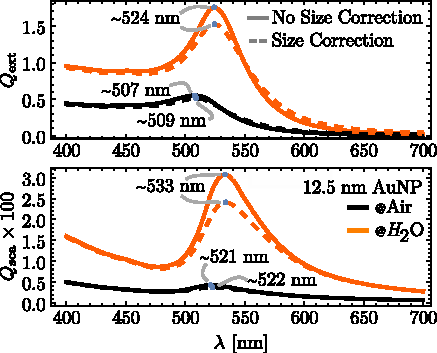
\includegraphics[scale = 1.02]{1-Theory/figs/QextQsca_12-5.pdf}\end{subfigure}
	\hspace*{-.5em}\begin{subfigure}{.05\textwidth}\vspace{-5.5cm}\caption{}\label{sfig:secondaty2}	\end{subfigure}
	\hspace*{-2.em}
	\begin{subfigure}{.48\textwidth} 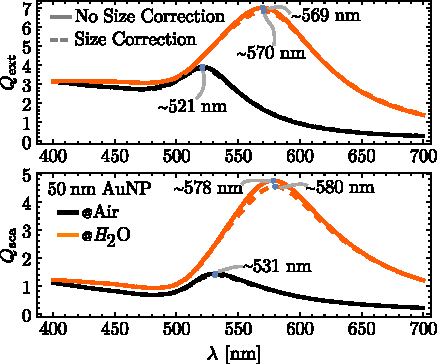
\includegraphics[scale = 1.02]{1-Theory/figs/QextQsca_50.pdf}\end{subfigure}%
\vspace*{-.5em}
\caption[Example of Figure title]{The explanation of your figures. \blindtext}	\label{fig:Main}
\end{figure}

\begin{figure}[h!]\centering
	
\includegraphics[scale=1]{1-Theory/figs/legend.pdf}\\[.5em]
%
	\hspace*{2em}\begin{subfigure}{.05\textwidth}\caption{}\label{sfig:secondary1}\vspace*{6.35cm}\end{subfigure}
	\hspace*{-3.50em}
	\begin{subfigure}{.24\textwidth} 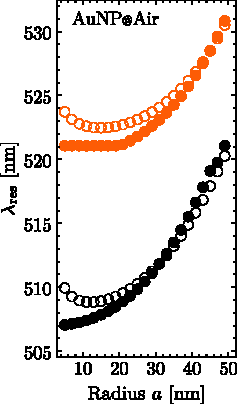
\includegraphics[scale = 1]{1-Theory/figs/redShift_rad1.pdf}\end{subfigure}
%
	\hspace*{.25em}\begin{subfigure}{.05\textwidth}\vspace{-6.35cm}\caption{}\label{sfig:secondaty2}	\end{subfigure}
	\hspace*{-2.5em}
	\begin{subfigure}{.24\textwidth} 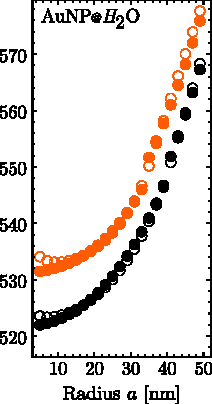
\includegraphics[scale = 1]{1-Theory/figs/redShift_rad2.pdf}\end{subfigure}%
%
	\hspace*{-.5em}\begin{subfigure}{.05\textwidth}\vspace{-6.35cm}\caption{}\label{sfig:secondaty2}	\end{subfigure}
	\hspace*{-2.45em}
	\begin{subfigure}{.24\textwidth} 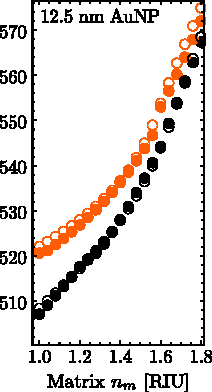
\includegraphics[scale = 1.02]{1-Theory/figs/redShift_mat1.pdf}\end{subfigure}%
%
	\hspace*{-.45em}\begin{subfigure}{.05\textwidth}\vspace{-6.35cm}\caption{}\label{sfig:secondaty2}	\end{subfigure}
	\hspace*{-2.45em}
	\begin{subfigure}{.24\textwidth} 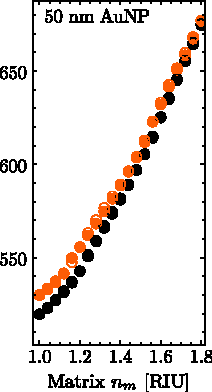
\includegraphics[scale = 1.02]{1-Theory/figs/redShift_mat2.pdf}\end{subfigure}%
\vspace*{-.5em}
\caption[Example of Figure title]{The explanation of your figures. \blindtext}
\label{fig:Main}
\end{figure}
\clearpage


	\section{Mie Scattering}
	  \label{s:Mie}

     In the previous Section, it was concluded that the extinction of light due to the interaction between a particle and a monochromatic plane wave can be determined through the amplitude of the scattered field in the forward direction. This is stated in the Optical Theorem, which is an exact relation, but inaccuracies may arise when either the scattering amplitude matrix or the extinction cross section are approximated\footnote{See for example Section 2.4 from Ref. \cite{tsang_scattering_2000} on the Rayleigh Scattering, and Section 21.7 from Ref. \cite{zangwill_modern_2013} on Thompson scattering.}. A particular case in which the scattering amplitude matrix can be exactly calculated is when the scatterer has spherical symmetry. In order to address this special case, it will be introduced a vectorial basis with spherical symmetry, known as the Vector Spherical Harmonics (VSH). Once the VSH are defined, they will be used to write a monochromatic plane wave in terms of the VSH. By imposing the continuity of the tangential components of the electric and magnetic fields, the scattered field can be also written in terms of the VSH. As a particular example of interest, shown in the last Section, the optical properties of a gold nanoparticle with radius of $12.5$ nm are calculated.

     % ------------------------------- index entries --------
     \index{Scattering!Thompson}%
     \index{Scattering!Mie}%
     \index{Scattering!Rayleigh}%
     \index{Vector!Spherical Harmonics}%

	    \subsection{Vector Spherical Harmonics}
		 \label{ss:VSH}
		 % !TeX root = ../tesis.tex

The electric and magnetic field, denoted as $\vb{E}$ and $\vb{B}$, respectively, are a solution to the homogeneous vectorial Helmholtz\index{Helmholtz!Equation, Vectorial} when an harmonic time dependence and a spacial domain with no external charge nor current densities is assumed, that is,
%
% -----------------------------
\begin{subequations}
\begin{tcolorbox}[title = Vectorial Helmholtz Equation,	ams align, breakable]
	\grad^2 \vb{E}(\vb{r},\omega) + k^2 \vb{E}(\vb{r},\omega) &= \vb{0},\\
  \grad^2 \vb{B}(\vb{r},\omega) + k^2 \vb{B}(\vb{r},\omega) &= \vb{0}.
\end{tcolorbox}
\label{eq:Helmholtz}
\end{subequations}
% ------------------------------
%
\noindent where the vectorial operator $\grad^2$ must be understood as $\grad^2 = \nabla(\nabla\cdot) - \nabla\times\nabla\times $, and $k$ is the wave number in the matrix. It is possible to build a basis set for the electric and magnetic fields as long as the elements of this basis are also solution to Eq. \eqref{eq:Helmholtz}. One alternative is to employ the following set of vector functions
%
% -----------------------------
\begin{subequations}
\begin{align}
	\vb{L} =& \nabla \psi,
	\label{eq:L}\\
	\vb{M} =& \nabla\times(\vb{r}\psi),
	\label{eq:M}\\
	\vb{N} =&  \frac{1}{k}\nabla\times\vb{M},
	\label{eq:N}
\end{align}%
\label{eq:VSH}%
\end{subequations}
% ------------------------------
%
that are solution to the homogeneous vectorial Helmholtz equation as long as the scalar function $\psi$ is solution to the scalar Helmholtz equation\footnote{%
	This result can be proven by considering the following: Let $f$ be $\mathcal{C}^3$ and $\vb{F}$ a $\mathcal{C}^2$. Then, it is true that $\nabla^2(\nabla f) = \nabla(\nabla^2 f)$, and $\curl(\grad^2\vb{F}) = \grad^2(\curl\vb{F})$. }\index{Helmholtz!Equation, Scalar}
%
% -----------------------------
\begin{align}
	\nabla^2 \psi + k^2 \psi = 0.
\label{eq:HelmoltzScalar}
\end{align}
% ------------------------------
%
The triad $\left\{\vb{L},\vb{M},\vb{N}\right\}$ is a set of vectors\footnote{%
	Employing the Einstein sum convention with $\epsilon_{ijk}$ the Levi-Civita symbol, Eq. \eqref{eq:M} can be the written as follows:%
	 	$M_i = [\nabla\times(\vb{r}\psi)]_i
	 	=  \epsilon_{ijk}\partial_j(r_k\psi)
	 	=\psi\epsilon_{ijk}\partial_j(r_k) -\epsilon_{ikj}r_k\partial_j\psi
	 	=\psi[\nabla\times\vb{r}]_i - [\vb{r}\times\nabla\psi]_i
	 	= - [\vb{r}\times\nabla\psi]_i
	 	= [\vb{L}\times\vb{r}]_i$,%
	 therefore $\vb{M}$ is orthogonal to $\vb{L}$ and $\vb{r}$. From Eq. \eqref{eq:N} $\vb{M}\cdot\vb{N}=0$, so $\vb{M}$ is orthogonal to $\vb{M}$. As it will be shown, not necessarily $\vb{L}$ is orthogonal to $\vb{N}$.
	}%
that obey Helmholtz equation \textit{i.e.}, they can be directly identify as electric or magnetic fields. The elements of the vector basis from Eq. \eqref{eq:VSH}   are known as the Vectorial Spherical Harmonics (VSH) as defined by  \citeauthor{stratton_electromagnetic_2012} \cite{stratton_electromagnetic_2012}, and \citeauthor{bohren_absorption_1983} \cite{bohren_absorption_1983} and the scalar function $\psi$ is known as the generating function of the VSH. From the definition of the VSH in Eqs. \eqref{eq:VSH} it can be seen that $\vb{L}$ has only a longitudinal component while $\vb{M}$ and $\vb{N}$ have only transversal components; specifically $\vb{M}$ is tangential to any sphere of radius $\norm{\vb{r}}$.


If spherical coordinates are chosen, and it is assumed that $\psi(r,\theta,\varphi) = R(r)\Theta(\theta)\Phi(\varphi)$, then Eq. \eqref{eq:HelmoltzScalar} can be decouple into three ordinary differential equations:
%
% ------------------------------
 \begin{align}
	\frac{1}{\Phi}\pdv[2]{\psi}{\varphi} &+ m^2 \Phi =0,
 \label{eq:Phi}\\
	\frac{1}{\sin\theta}\dv{\theta}\qty(\sin\theta\dv{\Theta}{\theta}) &+ \qty[\ell(\ell+1)- \frac{m^2}{\sin^2\theta}]\Theta =0,
	\label{eq:Theta}\\
	\dv{r}\qty(r^2\dv{R}{r}) &+ \qty[ (k r)^2 - \ell (\ell +1)] R =0,
 \label{eq:Req}
\end{align}	
% ------------------------------
%
where $\ell$ can takes natural values and zero, and $\abs{m}\leq \ell$ so $\Phi$ and $\Theta$ are univalued and finite on a sphere. Eqs. \eqref{eq:Theta} and \eqref{eq:Req} can be rewritten as
%
% ------------------------------
 \begin{align}
(1-\mu^2)\dv[2]{\Theta}{\mu} - 2\mu\dv{\Theta}{\mu} + \qty[\ell(\ell+1)-\frac{m^2}{1-\mu^2}]\Theta &= 0, \qqtext{ with $\mu = \cos\theta$,}
	\label{eq:ThetaMu}\\
	\rho\dv{\rho}\qty(\rho\dv{Z}{\rho}) +  \qty[\rho^2 - \qty(\ell + \frac12)^2]Z  &= 0,  \qqtext{ with $Z = R\sqrt{\rho}$ and $\rho = kr$.}
\label{eq:Reqkr}
\end{align}	
% ------------------------------
%
The solution to Eq. \eqref{eq:ThetaMu} are the associated Legendre functions $ P_\ell^m(\mu)$ and to Eq. \eqref{eq:Reqkr} the solution is given by the Spherical Bessel Functions of the first ($j_\ell$)  and second ($y_\ell$) kind, and the Spherical Hankel functions of first ($h_\ell^{(1)} = j_\ell + iy_\ell$) and second ( $h_\ell^{(2)} = j_\ell - iy_\ell$)  kind. Following the convention from most literature on Mie Scattering \cite{zangwill_modern_2013}, the solution to Eq. \eqref{eq:Phi} will be decompose in an odd ($o$) and an even ($e$) solution, that is, as sine and cosine functions, thus restricting the values of $m$ to non-negative integers. After this procedure, it is determined that the generating function of the VSH is given by
%
% -----------------------------
\begin{subequations}
\begin{tcolorbox}[title = $\psi$: Generating function of the vectorial spherical harmonics,	ams align, breakable]
	\psi_{e\ell m}(r,\theta,\varphi) =& \cos(m\varphi)P_\ell^m(\cos\theta)z_\ell(kr), 
	\label{eq:psiE}\\ 	
	\psi_{o\ell m}(r,\theta,\varphi) =& \sin(m\varphi)P_\ell^m(\cos\theta)z_\ell(kr).
	\label{eq:psiO}
\end{tcolorbox}
\label{eq:psi}
\end{subequations}
% ------------------------------
%
\noindent%
where $z_\ell$ stands for any of the four solutions to the radial equation [Eq. \eqref{eq:Reqkr}]. Substituting Eq. \eqref{eq:psiE} in Eqs. \eqref{eq:L}--\eqref{eq:N} one finds the even SVH
%
% -----------------------------
\begin{subequations}
\begin{tcolorbox}[title = Even vectorial spherical harmonics,	ams align, breakable]
	\vb{L}_{em\ell} =& k \cos(m\varphi)P_\ell^m(\cos\theta)\dv{z_\ell(kr)} {(kr)}\,\vu{e}_r 
					 +  k\cos(m\varphi) \frac{z_\ell(kr)}{kr}\dv{P_\ell^m(\cos\theta)}{\theta} \,\vu{e}_\theta \notag \\
					& - km \sin(m\varphi) \frac{P_\ell^m(\cos\theta)}{\sin\theta}\frac{z_\ell(kr)}{kr} \,\vu{e}_\varphi 
	\label{eq:Leml}\\
	\vb{M}_{em\ell} = &-m\sin(m\varphi)z_\ell(kr) \frac{P_\ell^m(\cos\theta)}{\sin\theta}\,\vu{e}_\theta
					-\cos(m\theta)z_\ell(kr) \dv{P_\ell^m(\cos\theta)}{\theta}(\cos\theta)\,\vu{e}_\varphi,
	\label{eq:Meml} \\
	\vb{N}_{em\ell} = &\cos(m\varphi) \frac{z_\ell(kr)}{kr} \ell(\ell+1)P_\ell^m(\cos\theta)\,\vu{e}_r 
						+ \cos(m\varphi)  \frac{1}{kr} \dv{[kr\, z_\ell(kr)] }{(kr)}
						\dv{P_\ell^m(\cos\theta)}{\theta}(\cos\theta)\,\vu{e}_\theta \notag\\
						&- m \sin(m\varphi) \frac{1}{kr} \dv{[kr\, z_\ell(kr)] }{(kr)}\frac{P_\ell^m(\cos\theta)}{\sin\theta}
		 \,\vu{e}_\varphi, 
	\label{eq:Neml}	
\end{tcolorbox}
\label{eq:SVHEven}
\end{subequations}
% ------------------------------
%
\noindent where the term $\ell( \ell+1)P_\ell^m$ arises since the associated Legendre functions obeys Eq. \eqref{eq:ThetaMu}. Likewise, the odd SVH are given by
%
% -----------------------------
\begin{subequations}
\begin{tcolorbox}[title = Odd vectorial spherical harmonics,	ams align, breakable]
	\vb{L}_{om\ell} =& k \sin(m\varphi)P_\ell^m(\cos\theta)\dv{z_\ell(kr)} {(kr)}\,\vu{e}_r 
					 +  k\sin(m\varphi) \frac{z_\ell(kr)}{kr}\dv{P_\ell^m(\cos\theta)}{\theta} \,\vu{e}_\theta \notag \\
					& +  km\cos(m\varphi) \frac{P_\ell^m(\cos\theta)}{\sin\theta}\frac{z_\ell(kr)}{kr} \,\vu{e}_\varphi 
	\label{eq:Loml}\\
	\vb{M}_{om\ell} = & m\cos(m\varphi)z_\ell(kr) \frac{P_\ell^m(\cos\theta)}{\sin\theta}\,\vu{e}_\theta
					-\sin(m\theta)z_\ell(kr) \dv{P_\ell^m(\cos\theta)}{\theta}(\cos\theta)\,\vu{e}_\varphi,	
	\label{seq:Moml} \\
	\vb{N}_{om\ell} =&\sin(m\varphi)\frac{z_\ell(kr)}{kr} \ell(\ell+1)P_\ell^m(\cos\theta)\,\vu{e}_r +
					 \sin(m\varphi)  \frac{1}{kr} \dv{[kr\, z_\ell(kr)]}{(kr)} \dv{P_\ell^m(\cos\theta)}{\theta}(\cos\theta) \,\vu{e}_\theta \notag\\
					 & + m \cos(m\varphi) \frac{1}{kr} \dv{[kr\, z_\ell(kr)]}{(kr)} \frac{P_\ell^m(\cos\theta)}{\sin\theta}¸\, \vu{e}_\varphi.
	 \label{seq:Noml} 
\end{tcolorbox}
\label{eq:SVHOdd}
\end{subequations}
% ------------------------------
%
\noindent%
The election on $z_\ell$ in Eqs. \eqref{eq:SVHEven} and  \eqref{eq:SVHOdd} is due to the physical constrains of the scattering problem. The spherical Bessel function of first kind, unlike the other three proposed solution to the radial equation, is finite in $r = 0$, thus it is appropriate for the internal electric field and plane waves. This election of $z_\ell$ will be denoted in the SVH with the superscript $(1)$. On the other hand, the asymptotic behavior of the Hankel function of first kind $h^{(1)} = j_\ell + i y_\ell$ is an outward spherical wave \cite{bohren_absorption_1983}, suited for the scattered field; the VSH with $z_\ell = h^{(1)}\ell$ will be then, denoted with the superscript $(3)$.

The SVH follow orthogonality relations inherited from the orthogonality of sine, cosine and the associated Legendre functions. Let us define the inner product as the integral in the solid angle between two vectorial functions as 
%
\begin{align}
\ev{\vb{A},\vb{A}'}_\Omega = \int_0^{2\pi}\int_0^{\pi} \vb{A}\cdot\vb{A}'\sin\theta\dd{\theta}\dd{\varphi}.
\label{eq:inner}
\end{align}
%
Under this inner product, all even SVH are orthogonal to the odd SVH due to the ortogonallity from the $\sin(m\varphi)$ and $\cos(m'\varphi)$, as well as all SVH  with $m\neq m'$. The remaining orthogonality relations are summarized in the following expressions \cite{stratton_electromagnetic_2012}
%
\begin{align}
\ev{\vb{L}_{em\ell},\vb{L}_{em\ell'}}_\Omega = \ev{\vb{L}_{om\ell},\vb{L}_{om\ell'}}_\Omega &= \delta_{\ell,\ell'}\frac{(1+\delta_{m,0})2\pi}{2\ell+1}\frac{(\ell+m)!}{(\ell-m)!}k^2\qty[ \ell z_{\ell-1}^2(kr) + (\ell+1)z_{\ell+1}^2(kr) ],\\
%
\ev{\vb{M}_{em\ell},\vb{M}_{em\ell'}}_\Omega = \ev{\vb{M}_{om\ell},\vb{M}_{om\ell'}}_\Omega &= \delta_{\ell,\ell'}\frac{(1+\delta_{m,0})2\pi}{2\ell+1}\frac{(\ell+m)!}{(\ell-m)!}\ell(\ell+1)z_{\ell}^2(kr),\\
%
\ev{\vb{N}_{em\ell},\vb{N}_{em\ell'}}_\Omega = \ev{\vb{N}_{om\ell},\vb{N}_{om\ell'}}_\Omega &= \delta_{\ell,\ell'}\frac{(1+\delta_{m,0})2\pi}{(2\ell+1)^2}\frac{(\ell+m)!}{(\ell-m)!}\ell(\ell+1)\qty[ (\ell+1) z_{\ell-1}^2(kr) + \ell z_{\ell+1}^2(kr) ]. \\
%%
\ev{\vb{L}_{em\ell},\vb{N}_{em\ell'}}_\Omega = \ev{\vb{L}_{om\ell},\vb{N}_{om\ell'}}_\Omega &= \delta_{\ell,\ell'}\frac{(1+\delta_{m,0})2\pi}{(2\ell+1)^2}\frac{(\ell+m)!}{(\ell-m)!}\ell(\ell+1)k\qty[ z_{\ell-1}^2(kr) - z_{\ell+1}^2(kr) ]. 
\end{align}
%


















































        \subsection{Incident, Scattered, and Internal Electric Fields}
	     \label{ss:Fields}
         % !TeX root = ../tesis.tex

 Let $\vb{E}^{\text{i}}$ be a $x$ polarized plane wave traveling in the vertical direction $\vb{e}_z$; its representation in the canonical spherical basis is
 %
 \begin{align}
 \vb{E}^{\text{i}} (\vb{r})= E_0\qty(\sin\theta\cos\varphi \vu{e}_r +
					\cos\theta\cos\varphi \vu{e}_\theta
					- \sin\varphi \vu{e}_\varphi) \exp(ikr\cos\theta).
	\label{eq:ExPlane}
 \end{align}
 %
The monochromatic plane wave is a transversal wave, thus it can be written in terms of only the VSH $\vb{M}^{(1)}$ and $\vb{N}^{(1)}$, where the radial dependency is given by $j_\ell$ since the monochromatic plane wave is finite everywhere. Even more, due to the dependency on $\varphi$, it is only restricted to values of $m = 1$. By inspection on the radial component of $\vb{E}^\text{i}$, proportional to $\cos\varphi$ it depends only on $\vb{N}_{e1\ell}^{(1)}$, and on the azimuthal component, proportional to $\sin\varphi$, it can depend only on $\vb{M}_{o1\ell}^{(1)}$. Thus, Eq. \eqref{eq:ExPlane} can be written as the linear combination of  $\vb{N}_{e1\ell}^{(1)}$ and $\vb{M}_{o1\ell}^{(1)}$. Through the orthogonality relations of the VSH, the $x$ polarized plane wave can be written as \cite{stratton_electromagnetic_2012}
  %
  \begin{subequations}
 \begin{align}
 \vb{E}^\text{i} (\vb{r})=& E_0 \sum_\ell\frac{i^\ell(2\ell+1)}{\ell(\ell+1)}\qty( \vb{M}_{o1\ell}^{(1)} -i \vb{N}_{e1\ell}^{(1)}),
\\
 \vb{H}^\text{i} (\vb{r})=& \frac{-kE_0}{\mu\omega} \sum_\ell\frac{i^\ell(2\ell+1)}{\ell(\ell+1)}\qty( \vb{M}_{e1\ell}^{(1)} +i \vb{N}_{o1\ell}^{(1)}).
 \end{align}%
 \label{eq:plane waveMultipole}%
   \end{subequations}%
%

In the problem of scattering due to a spherical particle of radius $a$, the continuity conditions on the parallel components on the electric and magnetic fields are written as
  %
 \begin{align}
 \qty(\vb{E}^\text{i} + \vb{E}^\text{sca}- \vb{E}^\text{int})\eval_{r=a}\times \vu{e}_r  =
  \qty(\vb{H}^\text{i} + \vb{H}^\text{sca} - \vb{H}^\text{int})\eval_{r=a} \times\vu{e}_r = 0,
  \label{eq:contuinity}
 \end{align}
 %
with  $\vb{E}^\text{sca}$ ( $\vb{E}^\text{int}$) the scattered (internal) electric field and  $\vb{H}^\text{sca}$ ( $\vb{H}^\text{int}$) the scattered (internal) magnetic field. If the incident field $\vb{E}^\text{i}$ is given by a $x$ polarized plane wave [Eq. \eqref{eq:ExPlane}] then the scattered and internal fields can be written also as a linear combination of $\vb{M}_{o1\ell}$ and $\vb{N}_{e1\ell}$. The internal field is finite inside the particle, thus the radial dependency is given by the function $j_\ell(k_p a)$ with $k_p$ the wave number inside the particle, while it is chosen the spherical Hankel function of first kind $h^{(1)}(ka)$  for the scattered fields due to its asymptotic behavior of a spherical outgoing wave, such election for the radial dependency is denoted by the superscript $(3)$ over the VSH. To simplify the following steps, the scattered and the internal electric files are proposed as
  %
  \begin{subequations}
 \begin{align}
 \vb{E}^\text{sca} (\vb{r})=& E_0 \sum_\ell\frac{i^\ell(2\ell+1)}{\ell(\ell+1)}\qty(i a_\ell \vb{N}_{e1\ell}^{(3)} -b_\ell \vb{M}_{o1\ell}^{(3)}),
 \label{eq:EscaLC}\\
 \vb{E}^\text{int} (\vb{r})=& E_0 \sum_\ell\frac{i^\ell(2\ell+1)}{\ell(\ell+1)}\qty( c_\ell\vb{M}_{o1\ell}^{(1)} - i d_\ell \vb{N}_{e1\ell}^{(1)}),
 \end{align}
 \label{eq:EscaInt}
 \end{subequations}
 %
% where the Hankel spherical functions has $\rho =$
with the respective magnetic fields
  %
    \begin{subequations}
 \begin{align}
 \vb{H}^\text{sca} (\vb{r})=& \frac{-kE_0}{\mu\omega} \sum_\ell\frac{i^\ell(2\ell+1)}{\ell(\ell+1)}\qty(i b_\ell \vb{N}_{o1\ell}^{(3)} +a_\ell \vb{M}_{e1\ell}^{(3)}),\\
 \vb{H}^\text{int} (\vb{r})=& \frac{-kE_0}{\mu_p\omega} \sum_\ell\frac{i^\ell(2\ell+1)}{\ell(\ell+1)}\qty( d_\ell\vb{M}_{e1\ell}^{(1)} + i c_\ell \vb{N}_{o1\ell}^{(1)}).
 \end{align}%
\label{eq:HscaInt}%
 \end{subequations}%
 %
Since only the term $m=1$ is taken into account, it is convenient to define the angular functions
%
\begin{align}
 \pi_\ell(\cos\theta )  = \frac{P_\ell^1(\cos\theta)}{\sin\theta},\qqtext{and}
 \tau_\ell(\cos\theta) = \dv{P_\ell^1(\cos\theta)}{\theta},
 \label{eq:PiTau}
\end{align}
%
which are not orthogonal but their addition and substraction are, that is $\pi_\ell \pm \tau_\ell$ are orthogonal functions \cite{bohren_absorption_1983}. After substitution  of Eqs. \eqref{eq:plane waveMultipole}, \eqref{eq:EscaInt} and \eqref{eq:HscaInt} into Eq. \eqref{eq:contuinity} and considering the orthogonality of the odd and even VSH, of the vectors $\vb{M}$ and $\vb{N}$, and of $\pi_\ell \pm \tau_\ell$, it is shown that the coefficients $a_\ell$, $b_\ell$, $c_\ell$ and $d_\ell$ are given by two decoupled equation systems
%
\begin{align}
\mqty([x h_\ell^{(1)}(x)]  & (\mu/\mu_p) [(mx) j_\ell(mx)] \\
		m[x h_\ell^{(1)}(x)]' & [(mx) j_\ell(mx)]')
		\mqty(a_\ell \\ d_\ell) = \mqty([xj_\ell(x)] \\ m[x j_\ell(x)]') ,
	\label{eq:syst1}
		\\
\intertext{and}
\mqty( m[xh_\ell^{(1)}(x)]  &  [(mx)j_\ell(mx)] \\
		[x h_\ell^{(1)}(x)]' & (\mu/\mu_p)[(mx) j_\ell(mx)]' )
		\mqty(b_\ell \\ c_\ell) = \mqty(m[xj_\ell(x)] \\ [x j_\ell(x)]'),
	\label{eq:syst2}
\end{align}
%
where $m = k_p / k = n_p / n_\text{m}$ is the contrast between the sphere and the matrix, $x= ka = 2\pi n_\text{m} (a/\lambda)$ is the size parameter and  ($'$) denotes the derivative respect to the argument of the spherical Bessel or Hankel functions. The Eqs. \eqref{eq:syst1} and \eqref{eq:syst2} are simplified when the Riccati-Bessel functions $\psi_\ell( \rho) = \rho j_\ell(\rho)$ and $\xi(\rho) = \rho h_\ell^{(1)}(\rho)$ are introduced.

When a no magnetic particle nor matrix are assumed  ($\mu_p = \mu = \mu_0$), the coefficients $a_\ell$ and $b_\ell$ are known as the Mie Coefficients whose expression is calculated by inverting  Eqs. \eqref{eq:syst1} and \eqref{eq:syst2}, leading to
% -----------------------------
\begin{subequations}
	\begin{tcolorbox}[title = Mie Coefficients, ams align, breakable ]
	a_\ell &= \frac{\psi_\ell(x)\psi_\ell' (mx)-m\psi_\ell(mx)\psi_\ell'(x)}
				{\xi_\ell(x)\psi_\ell'(mx)-m\psi_\ell(mx)\xi_\ell'(x)},
				\label{eqs:a_ell}\\[.5em]
	b_\ell &= \frac{m\psi_\ell(x)\psi_\ell' (mx)-\psi_\ell(mx)\psi_\ell'(x)}
			{m\xi_\ell(x)\psi_\ell'(mx)-\psi_\ell(mx)\xi_\ell'(x)}.
			 \label{eqs:b_ell}
	\end{tcolorbox}\label{eq:MieCoef}
\end{subequations}
% ------------------------------
\noindent
Likewise, the coefficients $c_\ell$ and $d_\ell$ are
% -----------------------------
\begin{subequations}
\begin{align}
	c_\ell &= \frac{-m\xi_\ell'(x)\psi_\ell(x)+m\xi_\ell(x)\psi_\ell'(x)}
			{m\xi_\ell(x)\psi_\ell'(mx)-\psi_\ell(mx)\xi_\ell'(x)},\\[.5em]
	d_\ell &= \frac{-m\xi'_\ell(x)\psi_\ell(x)+m\psi_\ell'(mx)\psi_\ell'(x)}
				{\xi_\ell(x)\psi_\ell'(mx)-m\psi_\ell(mx)\xi_\ell'(x)}.
\end{align}%
\label{eq:coeffInt}%
\end{subequations}\noindent%
% ------------------------------
%
Even though the coefficients of the linear combination for the scattered and internal fields were obtained by assuming an $x$ polarized incident field, due to the spherical symmetry of the problem, by applying the transformation $\varphi \to \varphi + \pi/2$  the same procedure is valid for a $y$ polarized incident field  \cite{bohren_absorption_1983}, therefore all quantities related to the scattered and the internal field can be expressed in terms of Eqs. \eqref{eq:MieCoef} and \eqref{eq:coeffInt}.

As discussed in Section \ref{section:AmpMatCrossSect}, the optical properties of a particle are codified into the scattering, absorption and extinction cross sections, quantities that can be calculated by means of the scattering amplitude matrix [Eq. \eqref{eq:ScatAmpMat}] and the Optical Theorem [Eq. \eqref{eq:Cext}]. Since the particle is spherical, it is convinient to exploit the symmetry of the problem  by decomposing the scattered electric field [Eq. \eqref{eq:EscaLC}] into components parallel and perpendicular to the scattering plane. To obtain the scattering amplitude matrix  expressed in an orthogonal base relative to the scattering plane ($\vu{e}_\parallel^s =\vu{e}_\theta$ and $\vu{e}_\perp^s=-\vu{e}_\varphi$) let us substitute the Mie Coefficients [Eq. \eqref{eq:MieCoef}] into Eq. \eqref{eq:EscaLC}  while rewriting the VSH $\vb{M}^{(3)}_{o1\ell}$  [Eq. \eqref{eq:Moml}] and $\vb{N}^{(3)}_{e1\ell}$ [Eq. \eqref{eq:Neml}] in terms of the Riccati-Bessel function  $\xi$ and its derivative:
%
\begin{subequations}\label{eq:Esca}%
\begin{align}
\vb{E}^\text{sca}\cdot\vu{e}_r &=  \frac{\cos\varphi}{(kr)^2}
								\sum_\ell^\infty E_0i^\ell(2\ell+1)
								ia_\ell \xi(kr)\pi_\ell(\cos\theta) \sin\theta ,
\label{eq:EscaR}\\
\vb{E}^\text{sca}\cdot\vu{e}^\text{sca}_\parallel &=  \frac{\cos\varphi}{kr}
								\sum_\ell^\infty E_0i^\ell\frac{2\ell+1}{\ell(\ell+1)}
						[i a_\ell\xi_\ell'(kr)\tau_\ell(\cos\theta)-b_\ell\xi_\ell(kr)\pi_\ell(\cos\theta)],
\label{eq:EscaTheta}\\
\vb{E}^\text{sca}\cdot\vu{e}^\text{sca}_\perp &=  \frac{\sin\varphi}{-kr}
								\sum_\ell^\infty E_0i^\ell\frac{2\ell+1}{\ell(\ell+1)}
						[i a_\ell\xi_\ell'(kr)\pi_\ell(\cos\theta)-b_\ell\xi_\ell(kr)\tau_\ell(\cos\theta)].
\label{eq:EscaMPhi}
\end{align}%
\end{subequations}
%
Following a similar procedure but substituting Eq. \eqref{eq:coeffInt} into Eq. \eqref{eq:EscaInt}, the internal electric field $\vb{E}^\text{int}$ can be rewritten also in terms of the Riccati-Bessel functions as

\begin{subequations}\label{eq:Eint}%
\begin{align}
\vb{E}^\text{int}\cdot\vu{e}_r &=  -\frac{\cos\varphi}{(kr)^2}
               \sum_\ell^\infty E_0i^\ell(2\ell+1)
               id_\ell \psi(kr)\pi_\ell(\cos\theta) \sin\theta ,
\label{eq:EintR}\\
\vb{E}^\text{int}\cdot\vu{e}^\text{sca}_\parallel &=  \frac{\cos\varphi}{kr}
               \sum_\ell^\infty E_0i^\ell\frac{2\ell+1}{\ell(\ell+1)}
           [-i d_\ell\psi_\ell'(kr)\tau_\ell(\cos\theta)+c_\ell\psi_\ell(kr)\pi_\ell(\cos\theta)],
\label{eq:EscaTheta}\\
\vb{E}^\text{int}\cdot\vu{e}^\text{sca}_\perp &=  \frac{\sin\varphi}{-kr}
               \sum_\ell^\infty E_0i^\ell\frac{2\ell+1}{\ell(\ell+1)}
           [-i d_\ell\psi_\ell'(kr)\pi_\ell(\cos\theta)+c_\ell\psi_\ell(kr)\tau_\ell(\cos\theta)].
\label{eq:EintMPhi}
\end{align}%
\end{subequations}


The scattering amplitude matrix relates the incident electric field to the scattered electric field in the far field regime, that its when $kr\gg 1$. Considering that the series of Eqs. \eqref{eq:EscaR}-\eqref{eq:EscaMPhi} converge uniformly, so all contributions after the sufficiently large  term $\ell_c$ of the sum can be neglected for all values of $kr$, the asymptotic  expressions for the $\xi$ Riccati-Bessel function and its derivative can be employed, which are \cite{bohren_absorption_1983}
%
\begin{align}
\xi(kr)\approx (-i)^\ell \frac{\exp(ikr)}{i},
\qqtext{and}
\dv{\xi(kr)}{(kr)} = (-i)^\ell \exp(ikr)\qty(\frac{1}{i kr} + 1),
\qqtext{when}
\ell_c^2\ll kr.
\label{eq:RBXiAssym}
\end{align}
%

Substituting Eq. \eqref{eq:RBXiAssym} into  Eqs. \eqref{eq:EscaR}-\eqref{eq:EscaMPhi} and depreciating all terms proportional to $(kr)^{-2}$ it leads to a zero radial electric field while
%
\begin{subequations}%
\begin{align}
\vb{E}^\text{sca}\cdot\vu{e}^\text{sca}_\parallel & \approx \frac{\exp(ikr)}{r}
\left\{\frac{i}{k}\sum_\ell^\infty \frac{2\ell+1}{\ell(\ell+1)}
						[a_\ell\tau_\ell(\cos\theta)+b_\ell\pi_\ell(\cos\theta)]
				\right\}E_0\cos\varphi,
\label{eq:EthetaSca}\\
\vb{E}^\text{sca}\cdot\vu{e}^\text{sca}_\perp &\approx \frac{\exp(ikr)}{r}
\left\{\frac{i}{k}\sum_\ell^\infty \frac{2\ell+1}{\ell(\ell+1)}
						[a_\ell\pi_\ell(\cos\theta)+b_\ell\tau_\ell(\cos\theta)]
				\right\}E_0(-\sin\varphi),
\label{eq:EphiSca}
\end{align}\label{eq:EFar}
\end{subequations}
%
where it can be identified that $\vb{E}^\text{i}\cdot \vu{e}^\text{i}_\parallel = E_0\cos\varphi$ and $\vb{E}^\text{i}\cdot \vu{e}^\text{i}_\perp = -E_0\sin\varphi$ for $\vb{E}^\text{i}$ a plane wave traveling along the $z$ direction with an arbitrary polarization. Finally, the Scattering Amplitude Matrix for a spherical particle can be obtained by comparing Eqs. \eqref{eq:EthetaSca} and \eqref{eq:EphiSca} with Eq. \eqref{eq:ScatAmpMat}, leading to
%
\begin{tcolorbox}[title = Scattering Amplitude Matrix for Spherical Particles, ams align, breakable ]
\mathbb{F}(\vu{k}^\text{sca},\vu{k}^\text{i})
            &= \mqty(\dfrac{i}{k}S_2(\theta) & 0 \\
			0 & \dfrac{i}{k}S_1(\theta)  ),
            \label{eq:FscaS}
\intertext{with  $\vu{k}^\text{sca} = \vu{e}_r$, $\vu{k}^\text{i} = \vu{e}_z$, $\cos\theta = \vu{k}^\text{sca}\cdot\vu{k}^\text{i}$  and}
S_1(\theta)  &= \sum_\ell^\infty \frac{2\ell+1}{\ell(\ell+1)}
						[a_\ell\tau_\ell(\cos\theta)+b_\ell\pi_\ell(\cos\theta)],
            \label{eq:S1}
\\
S_2(\theta) &= \sum_\ell^\infty \frac{2\ell+1}{\ell(\ell+1)}
						[a_\ell\pi_\ell(\cos\theta)+b_\ell\tau_\ell(\cos\theta)].
            \label{eq:S2}
\end{tcolorbox}
%
The scattering amplitude matrix $\mathbb{F}$ shows the symmetry of the system when written in the a base relative to the scattering plane direction, as it was stated in Sec. \ref{section:AmpMatCrossSect}. Since the scatterer is a spherical istropic NP,  $\mathbb{F}$ is a diagonal matrix in the base  $\{\vu{e}^\text{sca}_\parallel, \vu{e}^\text{sca}_\perp  \}$, that is, that the scattered electric field $\vb{E}^\text{sca}$ mantains the same polarization degree relative to the scattering plane than the incident electric field $\vb{E}^\text{i}$ that illuminates the spherical particle.


        \subsection{Optical Properties of a Single Spherical (Gold) Particle}
		 \label{ss:AuMie}

         In previous Sections, the general theory for the light scattering was developed, introducing the scattering amplitude matrix $\mathbb{F}$ [Eq. \eqref{eq:ScatAmpMat}]. Then, the particular problem of a spherical scatterer was addressed and explicit expressions for the scattered electric field [Eq. \eqref{eq:EFar}] and for $\mathbb{F}$ were obtained [Eq. \eqref{eq:FscaS}] in terms of the Mie coefficients $a_\ell$ and  $b_\ell$ [Eqs. \eqref{eq:MieCoef}], as well as the internal electric field inside the scatterer [Eq. \eqref{eq:Eint}] in terms of the coefficients $c_\ell$ and $d_\ell$ [Eqs. \eqref{eq:coeffInt}]. The  optical properties of a particle is related to the electric field outside the scatterer,  and can be studied within two different spatial regions: the near-field and the far-field regimes. The near-field region consists in the complete analytical solution of the scattered electric field [Eq. \eqref{eq:EscaLC}], while the far-field regime considers only the contributions proportional to $r^{-1}$, with $r$ the distance between the center of the scatterer and the measurement point; the optical properties in the far-field regime can be determined by the scattering amplitude matrix $\mathbb{F}$ itself.  In this last Section, the previous results are employed to calculate the optical properties of  a spherical gold nanoparticle (AuNP) with a radius of $12.5$ nm, either embedded in an of air or in a glass matrix, when it is illuminated by an incident plane wave with a wavelength $\lambda$.

            \subsubsection{Localized Surface Plasmons}
             \label{sss:LSPR}
             % !TeX root = ../tesis.tex

The optical properties of a particle, either in the near or the far field regime,  are determined by the Mie coefficients   $a_\ell$ and $b_\ell$ [Eq. \eqref{eq:MieCoef}] since the exact solution to the scattered electric field $\vb{E}^\text{sca}$ is a linear combination of the vector spherical harmonics (VSH) $\vb{N}^{(3)}_{\text{e}1\ell}$ and $\vb{M}^{(3)}_{\text{o}1\ell}$ [Eq. \eqref{eq:EscaLC}] modulated by  $a_\ell$ and $b_\ell$, respectively. Thus, the physical interpretation of each term $\ell$ in the linear combination, as well as of $\vb{N}^{(3)}_{\text{e}1\ell}$ and $\vb{M}^{(3)}_{\text{o}1\ell}$ can be determined by visualizing each one of them independently. By understanding the contribution of each term, the optical response of a particle illuminated by a plane wave can be studied in the near and far regime.

The Fig. \ref{fig:Multipoles} shows the decomposition of the the scatttered electric field  $\vb{E}^\text{sca}$ of a particle into its contributions proportional to $a_1$ [Fig. \ref{fig:VSH:a1}], $b_1$ [Fig. \ref{fig:VSH:b1}], $a_2$ [Fig. \ref{fig:VSH:a2}] and $b_2$ [Fig. \ref{fig:VSH:b2}], when the particle is illuminated by a $x$ polarized plane wave traveling in the $z$ direction. The vectorial behavior of the $a_\ell$ contributions to $\vb{E}^\text{sca}$ are given by the VSH $\vb{N}^{(3)}_{\text{e}\ell 1}$ and by $\vb{M}^{(3)}_{\text{o}\ell 1}$ for the $b_\ell$ contributions. The  scattered electric field  is evaluated at a spherical surface (gray sphere) larger than the scatter: the arrow stream on the spherical surface corresponds to the pointing direction of each contribution to $\vb{E}^\text{sca}$ parallel to the evaluation sphere, while the color code corresponds to the magnitude of the scattered electric field at each point; the solid shape at the center of each axis is a contour surface $\norm{\vb{E}^\text{sca}}$.
%

\begin{figure}[h!]
	\def\svgwidth{1\textwidth} \small
  \vspace*{3.0em}
  \hspace*{0.em}
    \begin{subfigure}{.24\textwidth}\caption{\centering $\vb{E}^\text{sca} \sim  i a_1 \vb{N}^{(3)}_{\text{e}11}$}\label{fig:VSH:a1}\end{subfigure}
  	\begin{subfigure}{.24\textwidth}\caption{\centering $\vb{E}^\text{sca} \sim  - b_1 \vb{M}^{(3)}_{\text{o}11}$}\label{fig:VSH:b1}\end{subfigure}
	\begin{subfigure}{.24\textwidth}\caption{\centering $\vb{E}^\text{sca} \sim  i a_2 \vb{N}^{(3)}_{\text{e}12}$}\label{fig:VSH:a2}\end{subfigure}
	\begin{subfigure}{.24\textwidth}\caption{\centering $\vb{E}^\text{sca} \sim  - b_2 \vb{M}^{(3)}_{\text{o}12}$}\label{fig:VSH:b2}\end{subfigure}
  \vspace*{-6.em}\\
  \includeinkscape{VSH/3-VSH}
  \vspace*{-2em}
  \caption[Multipolar Contributions to the Scattered Electric Field]{ Decomposition of the  scattered electric field $\vb{E}^\text{sca}$ into its contributions  proportional to \textbf{a)} $a_1$,  \textbf{b)}  $b_1$, \textbf{c)} $a_2$ and \textbf{d)} $b_2$ [see Eq. \eqref{eq:EscaLC}] when a particle (not shown) is illuminated by an $x$ polarized plane wave traveling in the $z$ direction. The scattered electric field $\vb{E}^\text{sca}$ is evaluated at a sphere larger than the particle: the arrow stream corresponds to the projection parallel to the evaluation sphere of $\vb{E}^\text{sca}$  and the color code corresponds to the magnitude of  $\vb{E}^\text{sca}$. A contour surface of the magnitude of $\vb{E}^\text{sca}$ is located at the center of each axis. }
\label{fig:Multipoles}
\end{figure}

The general effect of each contribution to the scattered electric field  $\vb{E}^\text{sca}$  can be understood by analyzing their the behavior around the points where the scattered electric field drops to  zero; such points are called nodes and are shown in dark bluish colors in  Fig. \ref{fig:Multipoles}. The number of nodes over the evaluation sphere (gray surface) is proportional to the chosen value of $\ell$, for example, if $\ell = 1$ [Figs. \ref{fig:VSH:a1} and \ref{fig:VSH:b1}] there is a pair of such nodes and if $\ell = 2$ [Figs. \ref{fig:VSH:a2} and \ref{fig:VSH:b2}] there are two pairs, where each pair consists of two nodes at opposite sides of the evaluation sphere. When comparing the contributions proportional to $a_\ell$ [Figs. \ref{fig:VSH:a1} and \ref{fig:VSH:a2}] and  to $b_\ell$ [Figs. \ref{fig:VSH:b1} and \ref{fig:VSH:b2}], one difference is the location of the pairs of nodes for a fixed value of $\ell$, which differ spatially by a rotation around the $z$ axis of an angle $\varphi = \pi/2$.  Another difference between the $a_\ell$ and the $b_\ell$ contribution to  $\vb{E}^\text{sca}$ are the trajectories they performed around each pair of nodes: the $a_\ell$ contributions the scattered electric field flows from one node to its pair, thus following an open path, while the scattered electric field for the $b_\ell$ contributions circulates around the nodes forming a closed path. Taking into account such behaviors of the scattered electric field, it can be seen that the $a_\ell$ ($b_\ell$) contribution describes the electric field of an electric (magnetic) dipole when $\ell = 1$ and of an electric (magnetic) quadrupole when $\ell = 2$. Extrapolating such behavior for an arbitrary $\ell$,  it can be concluded that the $a_\ell$ contributions to the scattered electric field, described by the VSH $\vb{N}^{(3)}_{\text{e}\ell 1}$ corresponds to the electric field of an electric multipole of order $\ell$, while the $b_\ell$ contribution, described by the VSH $\vb{M}^{(3)}_{\text{o}\ell 1}$, corresponds to the electric field of a magnetic multipole of order $\ell$.

The scattered electric field of a spherical particle can be written, according to Eq. \eqref{eq:EscaLC}, as a linear contribution of electric fields associated to electric and magnetic mulutipoles as shown in Fig. \ref{fig:Multipoles}, modulated by the Mie coefficients $a_\ell$ and $b_\ell$, respectively. The Mie coefficients [Eq. \eqref{eq:MieCoef}] have a dependency on the radius $a$ of the spherical particle, on the wavelength $\lambda$ of the incident plane wave, the matrix embedding the particle through its  refractive index $n_\text{mat} = \sqrt{\varepsilon_\text{m}/\varepsilon_0}$, with $\varepsilon_\text{m}$ its dielectric function, and on the material of the particle itself, also through its refractive index $n_\text{p} = \sqrt{\varepsilon_\text{p}/\varepsilon_0}$, where $\varepsilon_p$ is the dielectric function of the particle, which in general depends on the wavelength of the incident plane wave.


            \subsubsection{Far-Field Optical Properties}
             \label{sss:FarField}
             % !TeX root = ../tesis.tex


In Fig. \ref{fig:Mieefficiencies} the extinction  $Q_\text{ext}$ and the scattering  $Q_\text{sca}$ efficiencies of a gold NP (AuNP) with a radius of $a = 12.5$ nm (12.5 nm AuNP) are shown as function of the wavelength $\lambda$ of the incident plane wave illuminating the NP. Two matrices were considered in Fig. \ref{fig:Mieefficiencies}: a matrix of air with a refractive index of $n_\text{mat} = 1$ (black lines) and a matrix of glass with $n_\text{mat} = 1.5$ (orange lines).  The experimental dielectric function for Au reported by \citeauthor{johnson_optical_1972} \cite{johnson_optical_1972}  was employed to model the electromagnetic response of the spherical AuNP nevertheless, this data corresponds to a bulk sample, meaning that it may not reproduce the optical behavior of a NP since surface effects cease to be neglectable  due to their spacial dimensions \cite{noguez_surface_2007}.   In order to study  the optical properties of AuNP while considering  surface effects,  a size correction to the dielectric function of the AuNP was performed as described in Appendix \ref{app:SizeCorrection}. The efficiencies of the $12.5$ nm AuNP  taking into account a dielectric function with (dashed lines) and without (solid lines) a size correction were compared for both considered matrices; on each curve the wavelength of their maximum value is indicated. The value of $\lambda$ at which the extinction efficiency is maximum corresponds to the excitation wavelength of the Localized Surface Pasmon Resonance (LSPR), that is, the wavelength where the extinction of light occurs the most.

% -------------------------------------- Extinctintion and scattering efficiencies -------------------------------
% --------------------------------------          12.5 nm AuNP @ Air and @ glass   -------------------------------
% --------------------------------------               fig:Mieefficiencies         -------------------------------
\begin{figure}[h!]
	\def\svgwidth{1\textwidth} \small
  \vspace*{3.0em}
  \hspace*{-9.em}
    \begin{subfigure}{.46\textwidth}\caption{ }\label{fig:Mieefficiencies:a}\end{subfigure}
    \begin{subfigure}{.49\textwidth}\caption{ }\label{fig:Mieefficiencies:b}\end{subfigure}
  \vspace*{-6.em}\\
  \includeinkscape{Mie-Au/1-Efficiencies}
  \vspace*{-2em}
  \caption[Extinction and Scattering Efficency of a 12.5 nm Au Spherical NP embeded into Air and Glass]{ \textbf{a)} Extinction $Q_\text{ext}$ and \textbf{b)} scattering $Q_\text{sca}$ efficiencies of a 12.5 nm Au spherical NP embeded into air (black, $n_\text{mat} = 1$)  and into galss (orange, $n_\text{mat} = 1.33$), as function of the wavelength $\lambda$ of the incident plane wave.  The solid curves were calculated by considering no size effects on the dielectric function of the AuNP, while the dashed curves consider a size correction to it; the experimental data of \citeauthor{johnson_optical_1972} \cite{johnson_optical_1972} was employed.}
\label{fig:Mieefficiencies}
\end{figure}
% --------------------------------------               fig:Mieefficiencies         -------------------------------

From the extinction and scattering efficiencies in Fig. \ref{fig:Mieefficiencies}, two main spectral tendencies arises between these quantities: on the overall value of the efficiencies and on the spectral position of their maximum. Since the scattering efficiency is two orders of magnitude smaller than the extinction efficiency within the visible range, the main energy loss mechanism is absorption, as stated by the Optical Theorem [Eq. \eqref{eq:Cext}]. Even though the 12.5 nm AuNP absorbs more light than what it scatters, both phenomena are present. For example, when the  12.5 nm AuNP is embedded into air, the wavelengths at which it absorbs and scatters the most are $\sim 509$ nm and $\sim 522$ nm, respectively. When the AuNP is embedded into glass, the absorption of light is optimized at a wavelength of $\sim 535$ nm, while the scattering is optimized at $\sim 543$ nm. For both an air and a glass matrix, the wavelength of most scattering is redshifted relative to the wavelength of most absorption for each case: $\sim 15$ nm for air and $\sim 7$ nm for glass. The extinction and scattering have different spectral tendencies as already discussed, yet they share common characteristics   when the dependency on the embedding media is studied.

Both the scattering and the absorption efficiencies of a 12.5 nm AuNP present an overall enhancement within the visible range when the refractive index of the matrix, the embedding media,  increases. This can be seen in Fig. \ref{fig:Mieefficiencies} by comparing the black curves ($n_\text{mat} = 1$, air) with the orange curves ($n_\text{mat} = 1.5$, glass). The value of the extinction efficiency of a 12.5 nm AuNP  at the excitation wavelength of the LSPR for a matrix of glass is around five times larger than for a matrix of air, as it can bee seen in Fig. \ref{fig:Mieefficiencies:a}, while the maximum value of the scattering efficiency for a glass matrix is around eight times larger compared to the case of an air matrix, as shown in Fig. \ref{fig:Mieefficiencies:b}. The enhancement of the extinction and the scattering efficiency as function of the refractive index of the matrix can be understood by analyzing the size paramter $ x = (2 \pi / \lambda ) a n_\text{mat} $, which compares the size of the NP relative to the incident wavelength in the matrix: the larger the value of $x$, the bigger a NP can be considered inside such matrix. Since the size parameter is a linear function of $n_\text{mat}$, the AuNP embedded into glass optically responds like a larger NP than what it is in air, thus having a more significant contributiom from the scattering to the light extinction mechanism inside glass, as well as an increse in the absorption.

The extinction [Fig. \ref{fig:Mieefficiencies:a}] and the scattering [Fig. \ref{fig:Mieefficiencies:b}] efficiencies of the same system, a 12.5 nm AuNP embedded into a matrix of either air or glass, are different whether a size correction to the dielectric function of the AuNP is considered (dashed lines) or not (solid lines). On the one hand, there is a spectral shift of the LSPR excitation wavelength for both matrices of $\sim 2$ nm: the AuNP embedded into air redifts from $\sim 507$ nm (no size correction) to $\sim 509$ nm (size correction) and the AuNP embedded into glass blueshifts from $\sim 506$ nm to $\sim 535$ nm. The maximum value of $Q_\text{sca}$ redifts $\sim 1$ nm when considering the size correction of the dielectric function when the AuNP is embeded into air nevertheless, the wavelength of maximum scattering does not present neither a red nor a blueshift larger than $1$ nm. On the other hand, the value of the efficiencies around the wavelength where the absorption and the scattering is maximized decreases in all cases shown if Fig. \ref{fig:Mieefficiencies}.  This behavior can be explained by how the size correction is performed: as explained in Appendix \ref{app:SizeCorrection}, the surface effects are taken into account by introuducing a smaller mean free path for the free electrons inside the AuNP, therefore increasing the value of the damping constant and thus leading to a larger imaginary part for the dielectric functiones employed, which is related to the absorption mechanisms \cite{ibach_solid-state_2009}. The descrease in the efficiencies due to a size corrected dielectric function is more evident for a matrix out of glass than out of air, which is an effect explained by the size parameter $x$ since a more light absorbing dielectric function is employed into a AuNP which has the opical properties of a larger NP when it is embedded into glass than into air. From this analysis it can be concluded that the most notable effect of a size correction to the dielectric function of a NP is the decrease in the extinction and scattering efficiencies, while there is still a spectral shift of the LSPR, whose effect is less relevant the larger the size parameter is.

While the scattering efficiency $Q_\text{sca}$ is an integral quantity, that is, it describes the scattering in all directions of a plane wave traveling in the  direction $\vb{k}^\text{i}$ due to the interaction with a NP, the scattering amplitude matrix elements $S_1(\theta)$,  given  for a spherical NP by Eq. \eqref{eq:S1}, and  $S_2(\theta)$, by Eq. \eqref{eq:S2}, depict the  electric field $\vb{E}^\text{s}$, at a measurement angle $\theta$,  scattered by a NP polarized in a direction perpendicular ($\perp$) to the scattering plane and parallel ($\parallel$) to it, respectively. A radiation pattern helps to vizualize the behavior of $S_{1,2}(\theta)$, a dimensionless parameter such as the scattering efficiency, by plotting their squared modulus as function of $\theta$, as it is shown in for a 12.5 nm AuNP in Fig. \ref{fig:ScatteringMaps}, where $\abs{S_{1}(\theta)}^2$ (solid lines) and $\abs{S_2(\theta)}^2$ (dashed lines) are shown for two different scenarios: a AuNP embedded into air [Fig. \ref{fig:ScatteringMaps:a}, black curves]  illuminated  at a wavelength $\lambda = 522$ nm and a AuNP embedded into glass  [Fig. \ref{fig:ScatteringMaps:b}, orange curves]  illuminated at $\lambda = 543$ nm. The wavelengths of the incident plane wave corresponds to the value of $\lambda$ where $Q_\text{sca}$ is maximized for each matrix as seen in Fig. \ref{fig:Mieefficiencies}.

% --------------------------------------				 Scaattering Maps 	   ------------------------------
% --------------------------------------   12.5 nm AuNP @ Air and @ glass    ------------------------------
% --------------------------------------         fig:ScatteringMaps         -------------------------------
\begin{figure}[h!]
	\def\svgwidth{.9\textwidth} \small\centering
		\vspace*{3.25em}
		\hspace*{-.25\textwidth}
	\begin{subfigure}{.25\textwidth}%
		\caption{$\abs{S_{1,2}(\theta)}^2\times 10^4$} \label{fig:ScatteringMaps:a}%
		\end{subfigure}%
	\begin{subfigure}{.45\textwidth}%
		\caption{$\abs{S_{1,2}(\theta)}^2\times 10^3$}\label{fig:ScatteringMaps:b}%
		\end{subfigure}%
	\vspace*{-6.25em}\\
	\includeinkscape{Mie-Au/2-ScatteringMaps}
	\vspace*{-.5em}
	\caption[Radiation Pattern of a 12.5 nm Au Spherical NP embeded into Air and Glass]{Radiation pattern of a 12.5 nm Au spherical NP embeded into \textbf{a)} air illuminatated by a plane wave at a wavelength of $\lambda = 522$ nm and \textbf{b)} glass illuminated at $\lambda = 543$ nm; the wavlength in each case corresponds to the wavelength of maximum scattering (see Fig. \ref{fig:Mieefficiencies}). The solid (dashed) lines corresponds to the scattering matrix element $S_1$ ($S_2$) related to an incident electric field $\vb{E}^\text{i}$ travelling in the $\vb{k}^\text{i}$ direction  and polarized perpendicularly (prallel) to the page. It was considered for both matrices a size corretion to the experimental data of \citeauthor{johnson_optical_1972} \cite{johnson_optical_1972} for the electromagnetic response of the AuNP.}
	\label{fig:ScatteringMaps}
 \end{figure}
 % --------------------------------------         fig:ScatteringMaps         -------------------------------

The quantities $\abs{S_{1,2}(\theta)}^2$ for a 12.5 nm AuNP embedded into air ($n_\text{mat} = 1$, black curves) are one order of magnitude smaller  than into glass ($n_\text{mat} = 1.5$, orange curves), meaning that the AuNP scatters light less efficiently in air than in glass, which is consistent with the obtained values for the scattering efficiency $Q_\text{sca}$ in Fig. \ref{fig:Mieefficiencies}. On the angular dependency, the radiation pattern of the AuNP in both matrices follow the same tendencies: an homogeneous scattered electric field when the AuNP scatters the perpendicularly polarized incident electric field  $\vb{E}^\text{s}_\perp$ (continuous lines), and a two-lobes pattern when illuminated with a parallel polarized $\vb{E}^\text{i}$.



\chapter{The Finite Element Method}
 \label{chapter:FEM}

    Several physical problems are described by systems of partial differential equations (PDE) alongside boundary or initial conditions, whose analytical solution can be achieved only in some cases. For example, the scattering of light due to an arbitrary spherical particle, described by the vectorial Helmholtz equation [Eq. \eqref{eq:Helmholtz}] with the boundary conditions at the surface of the spherical particle given by Eq. \eqref{eq:contuinity},   is one of the few physical problems with an analytical solution. Nevertheless, it is set in an ideal scenario where the particle is a perfect sphere, it is isolated and embedded in a non-absorbing matrix. Any of  these conditions on the geometry and physical properties of the described system were to change, the scattering problem may not have an analytical solution;  for such cases one alternative is to employ a numerical approach to find an approximated solution.  Among the numerical methods employed in Electrodynamics, one of them is the Finite Element Method (FEM).

    In this Chapter the theory behind the FEM is presented with its implementation on the light scattering problem. In Section \ref{s:FEM-Fund} fundamentals of the FEM are explained: the Galerkin method and the concept of the finite element. In Section \ref{s:Scat-FEM}, the light scattering problem is revisited so it can be approached through an integral formulation, allowing the use of the FEM since a generalization of the concepts seen in Section \ref{s:FEM-Fund}  into vectorial quantities is needed, as well as the introduction of boundary conditions in open regions so an infinite medium problem, such as the light scattering, can be approached numerically. In the last section, the scattering problem of an isolated spherical particle, addressed in Chapter \ref{ch:OpticalProperties}, is solved analytically and numerically ---employing the commercial software COMSOL Multiphysics\texttrademark{} Ver. 5.4--- and their results are contrasted.

    \section{Fundamentals}
     \label{s:FEM-Fund}
     % !TeX root = ../tesis.tex

Any system of PDE describing a physical system in either equilibrium or in a steady-state, with a set of boundary conditions, can be described by \cite{dhatt_finite_2012}
%
\begin{align}
    \mathcal{L}[\vb{u}(\vb{r})] - \vb{f}_\Omega = 0,
    \qquad\qquad
    \mathcal{C}[\vb{u}(\vb{r})] = \vb{f}_{\partial\Omega},
\label{eq:PDESystem}
\end{align}
%
where $\mathcal{L}$ and $\mathcal{C}$ are differential operators applied on the unknown functions $\vb{u}$---a $D$ dimensional quantity--- evaluated at a point $\vb{r}$ in a domain $\Omega$ and its boundary $\partial\Omega$, respectively;  $\vb{f}_\Omega$ and $\vb{f}_{\partial\Omega}$ are known functions related to the sources of $\vb{u}$ and to its boundary conditions.  The description of the physical system as stated by Eq. \eqref{eq:PDESystem} is known as its strong formulation since $u$ must be $m$-times differentiable on $\Omega$ if $\mathcal{L}$ is a differential operator of order $m$ \cite{dhatt_finite_2012,larson_finite_2013}. It is possible to relax such differentiability condition on $\vb{u}$ by employing the weak formulation of the PDE system, which in an integral representation of Eq. \eqref{eq:PDESystem} obtained by multiplying it by a trial function $\psi$ and integrating on $\Omega$ \cite{dhatt_finite_2012,larson_finite_2013,fletcher_computational_1984}
%
\begin{align}
    W(u) = \int_\Omega \psi(\vb{r}) \left\{ \mathcal{L}[\vb{u}(\vb{r})] - \vb{f}_\Omega   \right\} \dd{\Omega} = \vb{0}.
    \label{eq:Weak}
\end{align}
%
The weak formulation of the PDE system yields a weak solution to $\vb{u}$ since Eq. \eqref{eq:Weak} can be rewritten by performing $s$-fold integration by parts and then  employing Gauss's Theorem or by employing Green's first identity \cite{larson_finite_2013}:
%
\begin{align}
    \int_\Omega \psi \nabla\cdot \vb{u}\dd{\Omega} &=  - \int_\Omega \nabla\psi \cdot \vb{u} \dd{\Omega} + \oint_{\partial\Omega} \psi \vb{u}\cdot \vu{n}\dd{(\partial\Omega)},
        & \mbox{(with Gauss's Theorem),}
        \label{eq:GT}
    \\
    \int_\Omega \vb{u}\cdot\nabla\psi \dd{\Omega} &=  - \int_\Omega \psi \nabla\cdot \vb{u}\dd{\Omega}  + \int_{\partial \Omega}\psi \vb{u}\cdot\vu{n}\dd{(\partial\Omega)},
        & \mbox{(Green's first identity).}
        \label{eq:G1I}
\end{align}
%
If  Eqs. \eqref{eq:GT} or \eqref{eq:G1I} are used $s$-fold on Eq. \eqref{eq:Weak} then $\vb{u}$ must be differentiable $m-s$ times instead of $m$, while $\psi$ must be $s$ times differentiable. More over, the boundary conditions imposed to $u$ must be satisfied only if they contain  derivatives up to the order $m-s-1$ since the conditions with derivatives of order bigger than $m-s$ are taken into account in the integrals of Eqs. \eqref{eq:GT} and \eqref{eq:G1I} ---and on such boundary conditions $\psi$ must equal zero---. Thus, any solution $\vb{u}$ to Eq. \eqref{eq:Weak} is known as a weak solution  since it does not holds the differentiability condition as they are required by the equivalent strong formulation \cite{dhatt_finite_2012}.

Among the several methods to find an approximated solution to Eq. \eqref{eq:Weak}, the Galerkin method is one of the most common and implemented methods alongside the finite element approximation, which together form the finite element method. To ease the key ideas of the Galerkin and the finite element approximation, the unknown function $\vb{u}$ is assumed to be a scalar quantity $u$ in the following section.

    \subsection{The Galerkin Method}

    To find an approximated solution to $u$, one option is to employ the weighted residual method, which changes the PDE system to an algebraic equation system by proposing an approximation  $\tilde{u}$ as a linear combination of $N$ known functions  $\phi_i$, which differs from the exact solution $u$ by an error $e_{u}$, that is \cite{dhatt_finite_2012,larson_finite_2013,fletcher_computational_1984}
     %
     \begin{align}
        {u}(\vb{r}) = \tilde{{u}}(\vb{r}) + e_{{u}}(\vb{r}),
            \qquad\qquad
            \text{with}
            \qquad\qquad
        \tilde{{u}}(\vb{r}) = \sum_{i = 1}^{N} {a}_i\phi(\vb{r}),
     \label{eq:uapprox}
     \end{align}
     %
     where $\tilde{{u}}$ follows the same boundary conditions as ${u}$ at $\partial\Omega$ and ${a}_i$ are $N$ parameters to be determined\footnote{The $N$ parameters ${a}_i$ are constant for equilibrium and steady-state problems while they may depend on time for transport problems \cite{dhatt_finite_2012}.}. The values of ${a}_i$ are chosen so that $e_{{u}}\ll  \tilde{u} $, which may be achieved by increasing $N$ or by choosing ${a}_i$ that match the exact value of ${u}$ at determined points.

     One particular form to the approximated solution $\tilde{u}$ in Eq. \eqref{eq:uapprox} is known as the nodal approximation \cite{dhatt_finite_2012, fletcher_computational_1984}:
     %
     \begin{align}
        \tilde{u}(\vb{r}) = \sum_{i = 1}^N u_i \phi_i(\vb{r}),
            \qquad
            \text{with}
            \qquad
        u_i = u(\vb{r}_i),
     \label{eq:Nodal}
     \end{align}
     %
     where  $\phi_i$ are the so called interpolating ---or shape--- functions and $u_i$ are coefficients that equals the exact value of the function $u$ at $N$ points $\vb{r}_j \in \Omega$, called the nodal points. From Eq. \eqref{eq:Nodal} it can be seen that the error $e_{u}$ between the exact and the approximated solutions vanishes at the nodes $\vb{r}_j$ and thus $\phi_i(\vb{r}_j) = \delta_{ij}$, with $\delta_{ij}$ the Kronecker delta.

      Since $\tilde{u}$ is an approximated solution, the evaluation fo Eq. \eqref{eq:Nodal} into Eq. \eqref{eq:PDESystem} equals to a residual $  R_{\tilde{u}}(\vb{r},\{u_i\}_{i\leq N}) $ which in general is different to zero \cite{fletcher_computational_1984,larson_finite_2013}, that is,
     %
     \begin{align}
         \mathcal{L}[\tilde{u}(\vb{r})] - {f}_\Omega = R_{\tilde{u}}(\vb{r},\{u_i\}_{i\leq N}) \neq 0.
     \label{eq:PDESystem-app}
     \end{align}
     %
     To determine the coefficients $u_i$, the residual $R_{\tilde{u}}$ is multiplied by a weighting ---or trial--- function $\psi_j$ and integrated over $\Omega$ imposing that the integral goes to zero, that is
     %
     \begin{align}
        W(\tilde{u}) = \int_\Omega \psi_j(\vb{r}) R_{\tilde{u}}(\vb{r},\{u_i\}_{i\leq N}) \dd{\Omega} = \vb{0}.
            \qquad\qquad
            \text{with}
            \qquad\qquad
        \psi_j \in \{\psi_j\}_{j\leq N},
     \label{eq:WRM}
     \end{align}
     %
     which is a set of $N$ independent algebraic equations with $N$ variables.  It is worth noting that Eq. \eqref{eq:WRM} equals Eq. \eqref{eq:Weak}, and thus $u = \tilde{u}$, if the trail functions are elements of an infinite set, that is, $N \to \infty$ \cite{dhatt_finite_2012}.

     The weighted residual method is a family of numerical methods defined by the election of the trial functions set $\{\psi_j\}_{j\leq N}$. Some of the most common election for the trial functions set yield the collocation method, the least-squares method ant  the method of moments, and the Galerkin method, all given by \cite{fletcher_computational_1984,dhatt_finite_2012}:
     %
     \begin{subequations}
         \label{eq:WRM-family}%
     \begin{align}
         \{\psi_j\}_{j\leq N} &= \{\delta(\vb{r}-\vb{r}_j)\}_{j\leq N},   &\text{(Collocation method)},\\
         \{\psi_j\}_{j\leq N} &= \{\pdv*{R_{\tilde{u}}}{u_j}\}_{j\leq N},   &\text{(Least-squares method)},\\
         \{\psi_j\}_{j\leq N} &= \{x^j\}_{j\leq N},   &\text{(Moments method)},\\
         \{\psi_j\}_{j\leq N} &= \{\phi_j\}_{j\leq N},   &\text{(Galerkin method)},
         \label{eq:Galerkin}
     \end{align}%
 \end{subequations}\noindent%
    %
    where the Galerkin method sets the trial functions equal to the interpolating functions. Comparing the methods shown in Eqs. \eqref{eq:WRM-family}, the Galerkin method returns an approximated solution with the highest accuracy while having a moderated ease to implementation \cite{fletcher_computational_1984}. Yet, another advantage of the Galerkin method is that, for a eigenvalue problem, it guarantees real eigenvalues  if the PDE system in Eq. \eqref{eq:PDESystem} describes a self-adjoint operator \cite{dhatt_finite_2012,jin_theory_2010}. By substituting Eq. \eqref{eq:Galerkin} into Eq. \eqref{eq:WRM}, and exploiting the linearity of the differential operator $\mathcal{L}$, the PDE system is transformed into an algebraic problem as follows:
    %
    \begin{subequations}%
        \label{eq:GalerkinMat}%
    \begin{tcolorbox}[title = The Galerkin Method, ams align, breakable ]
        \mathbb{A} \vb{u} &= \vb{f}
            \intertext{where the entries of the matrix $\mathbb{A}$, and vectors $\vb{u}$ and $\vb{f}$ are}
        A_{ij} = \int \phi_i(\vb{r}) \mathcal{L}[\phi_j(\vb{r})]\dd{\Omega},
            \qquad
        u_i =& u(\vb{r}_i),
            \qquad
            \text{and}
            \qquad
        f_j = \int f_\Omega \phi_j(\vb{r}) \dd{\Omega}.
        \label{eq:GalerkinInt}
    \end{tcolorbox}%
\end{subequations}%
    \noindent
    %

    The Galerkin method is defined by the election of trial functions according to Eq. \eqref{eq:Galerkin}, which are assumed to be linear independent so Eq. \eqref{eq:GalerkinMat} is a solvable system of algebraic equations for the nodes $u_j$ \cite{fletcher_computational_1984}. Additionally, due to a  better performance, it is recommended to choose the set of trial functions as the first $N$ elements of a complete set of functions in the domain $\Omega$ and to meet the boundary conditions on Eq. \eqref{eq:PDESystem} as exactly as possible \cite{fletcher_computational_1984}. It is also recommended for the functions $\phi_i$ to increase their polynomial order as the size of $\Omega$ grows since the integral in   Eq. \eqref{eq:GalerkinInt} can be calculated with higher accuracy if methods as quadrature are employed \cite{fletcher_computational_1984}.

    The Galerkin method returns an approximated solution $\tilde{u}$ to $u$, in the weak sense, as a linear combination of the interpolating functions $\{\phi_i\}_{i\leq N}$ so long the error $e_{u}$ can be depreciated for all points in the domain $\Omega$.  Such solution is determined by inverting the matrix $\mathbb{A}$ in Eq. \eqref{eq:GalerkinMat} thus, a crucial step is to find the set $\{\phi_i\}_{i\leq N}$ of functions to solve the problem in $\Omega$ that follows the boundary conditions on $\partial\Omega$.  From a computational approach, the required computing time and resources increase as $\Omega$ does, therefore requiring the cardinality of the sets $\{\psi_j\}_{j\leq N}$ and  $\{\phi_i\}_{i\leq N}$ to increase as well \cite{dhatt_finite_2012}. To overcome such problem, one alternative is to divide $\Omega$ into $M$ smaller subdomains allowing for low cardinality interpolating functions to solve Eq. \eqref{eq:WRM}  in each subdomain.  This method is known as the finite element approximation and it is discussed in the following section.


        \subsection{The Finite Element Approximation}
         \label{ss:FEM-FE}
         % !TeX root = ../tesis.tex



The finite element approximation allows the use of low order interpolating functions by defining the subdomains $\Omega_k$ such that
%
\begin{align}
    \bigcup_{k=1}^M \Omega_k = \Omega,
        \qquad
        \text{and}
        \qquad
    \bigcap_{k=1}^M \Omega_k = \emptyset,
\label{eq:finite}
\end{align}
%
that is that, all $\Omega_k$ together represent the original domain $\Omega$ and that they do not overlap nevertheless, the boundaries of the finite elements are shared by neighbouring elements \cite{dhatt_finite_2012}. Then, the finite element approximation restricts  $\tilde{u}_k$  ---the nodal approximation  on each subdomain--- to depend only on the nodal points on $\Omega_k$ and on its boundary $\partial\Omega_k$, while all $\tilde{u}_k$ must be continuos across $\partial \Omega_k$ and obey the  differentiability condition they are bound to, whether the strong or weak formulation is employed \cite{dhatt_finite_2012}.

A finite element $\Omega_k$ is a subdomain of $\Omega$ following Eq. \eqref{eq:finite} \cite{dhatt_finite_2012}  but its formal definition requires $\Omega_k$ to be a manifold embedded into $\Omega$, as well as to chose a polynomial function space on $\Omega_k$, and to define a collection of $N_k$ linear functionals $\mathcal{F}_{\ell_k}$ on $\Omega_k$ \cite{larson_finite_2013}. The description of $\Omega_k$ as a manifold determines its geometrical properties such as dimensionality, shape and curvature, while the polynomials function space sets the order of the interpolating functions $\{\phi_{i_k}\}_{i_k\leq N_k}$. By applying $\phi_{i_k}$ into  $\mathcal{F}_{\ell_k}$, a system of $N_k$ algebraic  equations is obtained:
%
\begin{align}
    \mathcal{F}_{\ell_k}[\phi_{i_k}] = \delta_{{\ell_k} {i_k}},
    \label{eq:linfunc}
\end{align}
%
from which the interpolating functions are determined. Since the $N_k$ linear functional imposes conditions on the interpolating functions, the $N_k$ corresponds to the number of degrees of freedom of the finite element \cite{larson_finite_2013}.

The finte element corresponds to a particular way of discretization of the domain $\Omega$ and thus it is convinient to define the manifold $\Omega_k$ by its geometrical nodes $\vb{r}_{m_k}$, which are a finite collection of  points in $\Omega_k$. In Fig. \ref{fig:FinEleEx} some examples\footnote{Eventhough the elements shown in Fig. \ref{fig:FinEleEx} are triangles (2D) and  traingular piramids (3D), their shapes can also be composed by squares and prisms; see \cite{dhatt_finite_2012} for a more detailed list.} of common finite elements in one, two and three dimensions are shown: a straight line segment, a triangular surface and a tetrahedron \cite{dhatt_finite_2012} . The markers corresponds to the geometrical nodes in $\Omega_k$, from which the red markers corresponds to the geometrical nodes that define the shape of $\Omega_k$, since the lines joining two of them are the edges of the finite elements in two and three dimensions. The finite element in Fig. \ref{fig:FinEleEx:a} are known as reference elements since they have boundaries with no curvature and their geometrical nodes on its edges are equally spaced \cite{dhatt_finite_2012,larson_finite_2013}.   Even so, the finite elements are, in general, of curvilinear shape, as shown in Fig. \ref{fig:FinEleEx:b},  which may be preferred over the reference elements for $\Omega$ with no Cartesian symmetries. It is possible to perform a transformation $T:T(\boldsymbol{\xi})\to\vb{r}$ on the reference elements ($\boldsymbol{\xi}$) to reshape it into the so-called real-space element ($\vb{r}$), which corresponds to the physical space where the Eq. \eqref{eq:WRM} is to be solve \cite{dhatt_finite_2012,fletcher_computational_1984}.  Let us recall that the choice of finite elements with straight or curvilinear boundaries is related to the discretization method of the domain $\Omega$. For example, were $\Omega$ a cylinder in 3D, the use of finite elements with straight boundaries arises an error due to truncation of $\Omega$ at its boundary, which can be minimized by increasing the number of finite elements, while curvilinear finite elements may fill such space without increasing the number of finite elements.

 \begin{figure}[h!]
    \centering
    \small
        \def\svgwidth{.8\textwidth}
        \includeinkscape{FEM-Theory/1-systems-Elements-orders}
        \vspace*{-15em}\\
    \hspace*{-.8\textwidth}
        \begin{subfigure}{\textwidth}\caption{ }\label{fig:FinEleEx:a}\end{subfigure}
        \vspace*{5em}\\
    \hspace*{-.8\textwidth}
        \begin{subfigure}{\textwidth}\caption{ }\label{fig:FinEleEx:b}\end{subfigure}
    \vspace*{6em}\\
 \caption[References an Real-space Finite Elements]{ \textbf{a)} Reference and \textbf{b)} real-space finite elements for one (line segment), two (triangular surface) and three (tetrahedron) dimensional domains. The geometrical nodes on each element are signalized by the blue markers and their edges corresponds to the lines between the red markers; the number of nodes along each edge defines the order of the element. The transformation $T$ reshapes the reference finite element from its coordinate system $\boldsymbol{\xi}$ into a real-space element $\vb{r}$. }
\label{fig:FinEleEx}
\end{figure}

The transformation $T$ is a change of coordinates from the coordinate system $\boldsymbol{\xi}$  of the reference finite element into the real-space system $\vb{r}$. The use of Eq. \eqref{eq:linfunc} in the reference elements yield the different kind of interpolating functions, which can be employed to solve the weak formulation of a PDE system [Eq. \eqref{eq:WRM}] by transforming the derivatives in the real space coordinate system by means of the jacobian matrix $\mathbbm{J}$, whose elements are $J_{ij} = \partial \xi_i/\partial r_j$, and its determinant, the jacobian, that is \cite{dhatt_finite_2012,fletcher_computational_1984}:
%
\begin{align}
    \pdv{r_i} = \pdv{\xi_i}{r_j} \pdv{\xi_j},
    \qquad
    \text{and}
    \qquad
    \dd{\Omega_k} \to \det[\mathbbm{J}]\dd{\Omega_k}.
\label{eq:jac}
\end{align}
%
The Eq. \eqref{eq:jac} sets a constriction into the discretization of the original domain $\Omega$ and its partition into finite elements, since the jacobian must be non singular ---different from zero--- in all points in $\Omega_k$, meaning that the transformation $T$ of the reference element into the real-space finite element is bijective \cite{dhatt_finite_2012,fletcher_computational_1984}. To avoid singular points in $\Omega_k$, the real-space finite element must not be deformed considerably when transformed into the reference element \cite{dhatt_finite_2012}.

In order to build the interpolating functions $\phi_{i_k}(\boldsymbol{\xi})$ in the reference finite element, the polynomial functions space on $\Omega_k$ must be chosen by selecting the number of geometrical nodes found along the  edges \cite{larson_finite_2013}, so that the boundary conditions are met. For example, if there are $m$ geometrical nodes on each edge, the finite element is said to be of order $m-1$ since a polynomial of order $m-1$ is guaranteed to pass through the values given to  $m$ nodes. For example, the reference finite elements in Fig. \ref{fig:FinEleEx:a} are a cubic order 1D finite element (three geometrical nodes along the edges), a quadratic order triangular finite element (2D shape with three node along the edges), and a linear tetrahedral finite element (3D volume with four triangular faces and two nodes at each edge).

Once the polynomial functions space on the manifold $\Omega_k$ is set, this can be spanned by the set of interpolating functions $\phi_{i_k}(\boldsymbol{\xi})$, that are determined by means of the $N_k$ linear functional  $\mathcal{F}_\ell$ \cite{larson_finite_2013}.   The election of the  linear functionals give rise to different sets of interpolating functions and thus different families of finite elements. For example, the linear functional given by
     %
\begin{align}
 \mathcal{F}^{L}_{\ell_k}[f(\boldsymbol{\xi})] = f(\boldsymbol{\xi}_{\ell_k}) ,
\label{eq:Lag}
\end{align}
%
with  $\boldsymbol{\xi}_{\ell_k}$ the $\ell_k$-th  geometrical nodes, from a collection of $n_k$, in the reference finite element, defines the Lagrange finite element family since the  interpolating functions obtained by employing Eqs. \eqref{eq:linfunc} and \eqref{eq:Lag} are the Lagrange polynomials \cite{larson_finite_2013,dhatt_finite_2012,fletcher_computational_1984}. The functional $\mathcal{F}^{L}_{\ell_k}$ is a point evaluation in the $N_k = n_k$  geometrical nodes, which imposes no condition on the derivatives of $\phi_{i_k}$ at the boundary of $\Omega_k$, therefore the Lagrange finite element family returns a set of $N_k = n_k$ interpolating functions with no continuous first derivative between finite elements. One linear functional which does return interpolating functions with continuous first derivatives is the following:
%
\begin{align}
     \mathcal{F}^{H}_\ell[f(\boldsymbol{\xi})] = f(\boldsymbol{\xi}_{\ell_k}) ,
     \qquad
     \text{and}
     \qquad
     \mathcal{F}^{H}_{\ell_k'}[f(\boldsymbol{\xi})] = \vu{t}\cdot\nabla  f(\boldsymbol{\xi}_{\ell_k'}) = 0,
\label{eq:Her}
\end{align}
%
with $\boldsymbol{\xi}_{\ell_k}$ on of the $n_k$ geometric nodes in $\Omega_k$, $\boldsymbol{\xi}_{\ell_k'}$ one of the $n_k'$  geometric nodes at vertices of $\Omega_k$, and $\vu{t}$ is a unit vector parallel to its edges \cite{larson_finite_2013}. The functional in Eq. \eqref{eq:Her} give rise to the Hermite finite element family since the resulting interpolating functions are the Hermite polynomials, which allows for a solution on $\Omega$ 1-differentiable due to its $N_k = n_k + \times n'_k$ degrees of freedom \cite{dhatt_finite_2012,larson_finite_2013}. The Lagrange and the Hermite finite element families are two of the most common and simple nevertheless, one can build yet another family known as the serendipity finite element family  if the geometrical nodes outside the boundary of $\Omega_k$ are not considered in Eq. \eqref{eq:Lag} \cite{fletcher_computational_1984}. In Fig. \ref{fig:ExampleElements} the interpolating functions for a one and two dimensional finite elements under the Lagrange linear functional [Eq. \eqref{eq:Lag}] are shown:  a one dimensional cubic finite reference element [Fig. \ref{fig:ExampleElements:a}] and a serendipity triangular reference finite element of quadratic order.

\begin{figure}[t!]
    \hspace*{-.5\textwidth}
    \vspace*{7.5em}%
     \begin{subfigure}{\textwidth}\caption{ }\label{fig:ExampleElements:a}\end{subfigure}\\
    \hspace*{-.7\textwidth}
     \begin{subfigure}{\textwidth}\caption{ }\label{fig:ExampleElements:b}\end{subfigure}
     \vspace*{-11.5em}\\
    \centering
    \scriptsize
    \def\svgwidth{.9\textwidth}
    \includeinkscape{FEM-Theory/2-Example-Elements-2D}
\caption[Example of interpolating functions for 1D and 2D finite element]{Interpolating functions of \textbf{a)} a Lagrange cubic 1D reference finite element and \textbf{b)} a serendipity Lagrange quadratic 2D triangular reference element. The markers corresponds to the evaluation of the linear functionals [Eqs. \eqref{eq:linfunc} and $\eqref{eq:Lag}$] on the interpolating functions on each case.}
\label{fig:ExampleElements}
\end{figure}


    \section{Numerical Approach to the Light Scattering Problem}
     \label{s:Scat-FEM}

    In Chapter \ref{ch:OpticalProperties} the general theory of isolated scatterers in a non-absorbing media was developed and the particular case of spherical scatterers was approached analytically. In order to solve the light scattering problem through numerical methods and thus allowing for more complex geometries, the fundamentals of the Finite Element Method (FEM) were introduced in Section \ref{s:FEM-Fund}. Hereby, it is discussed the implementation of the FEM into the light scattering problem to find numerical approximations, in the weak sense, to the  electric field $\vb{E}(\vb{r})$ in finite domain $\Omega$. Due to the vectorial nature of the electric field, the interpolating ---and trial--- functions employed in the Galerkin method [Eq. \eqref{eq:GalerkinMat}] are chosen to be vectorial functions instead of scalar functions, since a family of vectorial finite element can be chosen so the boundary conditions of the electric fields are easily met. In this Section, the strong and weak formulations of the scattering of light are developed by employing such vectorial interpolating functions, and the corresponding finite elements are introduced, as well as the matrix representation of the light scattering problem. Lastly, additional conditions are imposed into the light scattering problem in order to solve it numerically through the FEM.

        \subsection{Strong and Weak Formulations}
         \label{ss:Scat-Form}
         % !TeX root = ../tesis.tex

The scattering light problem addressed in chapter \ref{ch:OpticalProperties} corresponds to a steady-state problem in a domain $\Omega$ whose optical properties are characterized by its electric permittivity $\varepsilon$ and magnetic permeability $\mu$, which in general are functions of the angular frequency $\omega$. To obtain the strong formulation of the light scattering, let us assume harmonic time dependent electric $\mathbfcal{E}(\vb{r},t)$ and magnetic fields $\mathbfcal{H}(\vb{r},t)$:
%
\begin{align}
    \mathbfcal{E}(\vb{r},t) = \vb{E}(\vb{r})\exp(-i\omega t),
        \qquad
        \text{and}
        \qquad
    \mathbfcal{H}(\vb{r},t) =  \vb{H}(\vb{r}) \exp(-i\omega t),
\end{align}
%
with $ \vb{E}(\vb{r})$ and $ \vb{H}(\vb{r})$ complex valued vectors. For harmonic time dependent EM fields, the Maxwell's equation are rewritten as \cite{jin_theory_2010,larson_finite_2013}
%
\begin{subequations}
    \label{eq:MaxwellsEq}
\begin{align}
    \nabla \cdot \qty(\varepsilon \vb{E})  &= \rho_\text{ext},  &\mbox{(Electric Gauss' law)},\\
    \nabla \cdot   \vb{B} &= 0, & \mbox{(Magnetic Gauss' law)},
            \label{eq:GaussM}\\
    \nabla \times \vb{E}  &= i\omega \mu \vb{H},  &  \mbox{(Faraday-Lenz's law)},\\
    \nabla \times \vb{H}  &= \vb{J} - i\omega \varepsilon \vb{E}, & \mbox{(Ampère-Maxwell' law)},
\end{align}
\end{subequations}
%
where  $\rho_\text{ext}$ is the external volumetric charge density, $\vb{J}$ is the volumetric current density and  $\vb{B} = \mu \vb{H}$. THe volumetric current density is given by \cite{larson_finite_2013}
%
\begin{align}
    \vb{J}(\vb{r},t) = \vb{J}_\text{ext}(\vb{r})\exp(-i\omega t) + \sigma \vb{E}(\vb{r})\exp(-i\omega t).
    \label{eq:ohmic}
\end{align}
%
where the $\vb{J}_\text{ext}$ corresponds to external current density, $\sigma$ is the frequency dependent conductivity of the domain $\Omega$ and the term $\sigma \vb{E}(\vb{r})\exp(-i\omega t)$ arises from a ohmic response of the domain $\Omega$.

The Maxwell's equations can be decouple to avoid working with two unknown functions, yielding \cite{jin_theory_2010,larson_finite_2013,bondeson_computational_2005}
%
\begin{align}
    \nabla \times \qty[\mu^{-1} \nabla \times \vb{E}] -(i\omega\sigma + \omega^2 \varepsilon) \vb{E} = i\omega \vb{J}_\text{ext}.
    \label{eq:curlcurlE}
\end{align}
%
which is another formulation of the vectorial Helmholtz equation [Eq. \eqref{eq:Helmholtz}]. The Eq. \eqref{eq:curlcurlE} is obtained by isolating $\vb{H}$ in the Faraday-Lenz's law, calculating its curl and, then, substituting  with the Ampère-Maxwell law and the Eq. \eqref{eq:ohmic}. In the absence of an external current and charge densities, Eq. \eqref{eq:curlcurlE} becomes the Maxwell eigenvalue problem \cite{larson_finite_2013}, which corresponds to the strong formulation of the light scattering problem alongside the  boundary conditions stated by Maxwell's equations [Eqs. \eqref{eq:MaxwellsEq}]. Therefore, the strong formulation of the light scattering problem is given by \cite{larson_finite_2013,jin_theory_2010,bondeson_computational_2005}
%
\begin{subequations}
    \label{eq:Scatt-Strong-All}
\begin{tcolorbox}[title = Maxwell eigenvalue problem and boundary conditions (Strong formulation), ams align, breakable ]
    \nabla \times \qty[\mu^{-1} \nabla \times \vb{E}] - \kappa^2 \vb{E} &= 0,
        &
        \text{with}
        \qquad
        \kappa^2 = (i\omega\sigma +\omega^2 \varepsilon),
    \label{eq:MaxwellEigenvalue}
    \\
    \vu{n}\times \vb{E}(\vb{r})\eval_{\partial \Omega} &= \vb{E}_\text{D},
        &\mbox{(Dirichlet Boundary Condition )},
    \label{eq:Dirichlet}
    \\
    \mu^{-1} \nabla \times \vb{E} \times \vu{n} \eval_{\partial \Omega} &=  \vb{E}_\text{N},
        &\mbox{(Neumann Boundary Condition)},
    \label{eq:Neumann}
\end{tcolorbox}
\end{subequations}
%
\noindent
with $\partial\Omega$ the boundary of $\Omega$ and $\vu{n}$ a normal vector to $\partial\Omega$. A Dirichlet type boundary condition is described in Eq. \eqref{eq:Dirichlet} while the Eq. \eqref{eq:Neumann} corresponds to Neumann type boundary condition. Both of such boundary condition are  equivalent to Eq. \eqref{eq:contuinity} in section \ref{ss:Fields} when  $\vb{E}_\text{D} =  \vb{E}_\text{N} = \vb{0}$.

In order to build the  weak formulation of the light scattering problem let us choose a set of $N$ linearily independent vectorial interpolating functions $\{\boldsymbol{\eta}_j\}_{j\leq N}$. If the Eq. \eqref{eq:MaxwellEigenvalue} is projected onto one interpolating function $\boldsymbol{\eta}_j$ and the resulting is integrated in the domain $\Omega$, one obtains
%
\begin{align}
    \int_\Omega \boldsymbol{\eta}_j\cdot \nabla \times \qty[\mu^{-1} \nabla \times \vb{E}] \dd{\Omega}
        = \int_\Omega \kappa^2 \boldsymbol{\eta}_j \cdot   \vb{E}  \dd{\Omega}.
    \label{eq:int-Scatt}
\end{align}
%
The left-hand side of Eq. \eqref{eq:int-Scatt} can be simplified by employing the vectorial identity $\nabla\cdot(\vb{A}\times \vb{B}) = \vb{B}\cdot\nabla\times\vb{A}-\vb{A}\cdot\nabla\times\vb{B}$, with $\vb{A} = \boldsymbol{\eta}_j$ and $\vb{B} = \mu^{-1}\nabla\times\vb{E}$, and performing a one-fold integration by parts, yielding
%
\begin{align}
    \int_\Omega \boldsymbol{\eta}_j\cdot \nabla \times \qty[\mu^{-1} \nabla \times \vb{E}] \dd{\Omega}
        =&  \int_\Omega \qty(\mu^{-1}\nabla\times\vb{E})\cdot \qty(\nabla\times\boldsymbol{\eta}_j)\dd{\Omega} +
            \notag \\
        & - \oint_{\partial\Omega}\qty[\boldsymbol{\eta}_j\times\qty(\mu^{-1}\nabla\times\vb{E})]\cdot \vu{n}\dd{(\partial\Omega)},
    \label{eq:IntParts}
\end{align}
%
where the last term in the right-hand side is obtained by the Gauss's Theorem. Substituting Eq. \eqref{eq:int-Scatt} into Eq. \eqref{eq:IntParts} and applying the boundary condition given by Eq. \eqref{eq:Neumann}, the Maxwell eigenvalue problem in its weak formulation is obtained:
%
\begin{subequations}
    \label{eq:Scatt-Weak-All}
\begin{tcolorbox}[title = Maxwell eigenvalue problem and boundary conditions (Weak formulation), ams align, breakable ]
    \int_\Omega \left\{\qty(\mu^{-1}\nabla\times\vb{E})\cdot \qty(\nabla\times\boldsymbol{\eta}_j) -  \kappa^2  \cdot   \vb{E} \cdot \boldsymbol{\eta}_j \right\} \dd{\Omega} & - \oint_{\partial\Omega} \qty(\boldsymbol{\eta}_j\times \vb{E}_\text{N})  \cdot\vu{n}\dd{(\partial\Omega)} = 0,
    \label{eq:MaxwellEigenvalue-weak}
    \\
    \vu{n}\times \vb{E}(\vb{r})\eval_{\partial \Omega} &= \vb{E}_\text{D}.
    \label{eq:Dirichlet-weak}
\end{tcolorbox}
\end{subequations}
%

The weak formulation problem of light scattering  [Eq. \eqref{eq:MaxwellEigenvalue-weak}] in the finite element approximation is reduced to the algebraic system of equations given by the Galerkin Method in each one of the $M$ subdomains $\Omega_k$ of $\Omega$ given by \cite{larson_finite_2013,jin_theory_2010}
%
\begin{subequations}
        \label{eq:Vec-FEM}
\begin{align}
    \mathbb{A} \vb{e} = \vb{0},
\end{align}%
with
\begin{align}
    A_{ij}  =     \int_{\Omega_k} \left\{\qty(\mu^{-1}\nabla\times\boldsymbol{\eta}_i)\cdot \qty(\nabla\times\boldsymbol{\eta}_j) -  \kappa^2  \cdot   \boldsymbol{\eta}_i \cdot \boldsymbol{\eta}_j \right\} \dd{\Omega_k}
            -& \oint_{\partial\Omega} \qty(\boldsymbol{\eta}_j\times \vb{E}_\text{N}) \cdot\vu{n}\dd{(\partial\Omega)},
\end{align}%
\end{subequations}%
\noindent%
%
where $A_{ij}$ are the matrix element of $\mathbb{A}$ and  $\vb{e}$ is the vector containing the $N$ coefficients of the linear combination of the interpolating function $\boldsymbol{\eta}_j$ that results into a approximated solution $\tilde{\vb{E}}(\vb{r}) = \sum_i e_i \boldsymbol{\eta}_j(\vb{r})$ to the electric field. The election of the coefficients $e_i$, its physical interpetation, and the set of the vectorial interpolating functions  is discussed in the next section.


         \subsection{The Nédélec Finite Element Family}
          \label{ss:Nedelec}
         % !TeX root = ../tesis.tex

 In order to perform the vectorial finite element approximation in Eq. \eqref{eq:Vec-FEM} equivalently to the scalar method in Eq. \eqref{eq:GalerkinInt}, an approximation $\tilde{\vb{E}}$ to the electric field $\vb{E}$ is proposed as linear combination of the vectorial interpolating functions $\boldsymbol{\eta}_j$ with scalar coefficients $e_i$. If the nodal approximation [Eq. \eqref{eq:Nodal}] were used for linear combination setting the coefficients $e_i$ as the exact solution of each component of  electric field at some nodal points into the finite element $\Omega_k$, not only the boundary condtion in Eq. \eqref{eq:Dirichlet-weak} might be diffuclt to meet \cite{larson_finite_2013,jin_theory_2010}, but also  some non-physical solutions may arise \cite{bondeson_computational_2005}. Therefore, instead of employing the nodal approximation, the expression of $\tilde{\vb{E}}$ in a finite element $\Omega_k$ of $\Omega$ is given by \cite{larson_finite_2013}
%
\index{Approximation!Nodal!Vectorial}%
\index{Partial Differential Equation (PDE)!Nodal Approximation!Vectorial}
\index{Partial Differential Equation (PDE)!Nodal Approximation!Vectorial!Interpolating Function $\boldsymbol{\eta}$}
\index{Functions!Interpolating $\boldsymbol{\eta}$}
%
\begin{align}
    \tilde{\vb{E}}(\vb{r}) = \sum_{i_k} e_{i_k} \boldsymbol{\eta}_{i_k}(\vb{r}),
        \qquad
        \text{with}
        \qquad
    e_{i} = \vu{t}_{i_k}\cdot \vb{E}(\vb{r}\in E_{i_k}),
\end{align}
%
where $E_{i_k}$ is the ${i_k}$-th edge in $\Omega_k$, $\vu{t}_{i_k}$ is a unitary vector  parallel to $E_{i_k}$ and $e_{i_k}$ is the exact value of the tangential component of the electric field on it. If the interpolating functions  $\boldsymbol{\eta}_{i_k}$ in the element $\Omega_k$ are to follow Eq. \eqref{eq:Dirichlet}, they  must have a continuous tangential components across $\partial\Omega_k$, while no special requirement is asked for their normal component on $\partial\Omega_k$. A special family of vectorial ---or edge--- reference finite elements are given by the linear functional \cite{larson_finite_2013}
%
\index{Finite Element!Linear Functional!Nédélec}
%
\begin{align}
    \mathcal{F}^{N}_{i_k}[\boldsymbol{\eta}_{\ell_k}(\boldsymbol{\xi})] = \frac{1}{\abs{E_{i_k}}}\qty(\int_{E_{i_k}} \vu{t}_{i_k}\cdot\boldsymbol{\eta}_{\ell_k}(\boldsymbol{\xi})   \dd{(\partial\Omega_k)} )^{1/2}  = \delta_{{i_k}{\ell_k}},
    \label{eq:Nedelec}
\end{align}
%
which is the square-root mean value of the interpolating function along the edge $E_{i_k}$. The reference finite elements obtained from Eq. \eqref{eq:Nedelec} are known as the Nédélec finite element of lowest order since their only degree of freedom is on the edges of the finite element \cite{bergot_generation_2010}. For triangular and tetrahedral finite elements, a closed formula for $\boldsymbol{\eta}_{i_k}$ is given by \cite{jin_theory_2010,larson_finite_2013,bondeson_computational_2005}
%
\begin{align}
    \boldsymbol{\eta}_{i_k} = \abs{E_{i_k}} \qty(\phi_{j_k}\nabla\phi_{\ell_k}
                                                    - \phi_{\ell_k}\nabla\phi_{j_k} ),
    \label{eq:NedelecTRi}
\end{align}
%
\index{Functions!Interpolating $\phi$!Lagrange}
%
with cyclic permutation of the indices $\{i_k, j_k, \ell_k\}$, corresponding to the vertices of triangular surfaces forming  the edges of the reference element. The scalar functions $\phi_{j_k}$ in Eq. \eqref{eq:NedelecTRi}  are the interpolating functions obtained with the Lagrange linear operator [Eq. \eqref{eq:Lag}] applied on $\Omega_k$ at the vertices. Nédélec finite elements of higher orders can be obtained if, additionally, more degrees of freedom are set to the faces and the volume of $\Omega_k$ \cite{bergot_generation_2010} nevertheless, their implementation is of greater difficulty and thus, less common \cite{larson_finite_2013,jin_theory_2010}. An example of Nédélec finite elements of lowest order are shown in Fig. \ref{fig:Nedelec:a} for a triangular finite element and in Fig. \ref{fig:Nedelec:b} for a tetrahedral finite element; the edge where Eqs. \eqref{eq:Nedelec} and \eqref{eq:NedelecTRi} are applied to is shown with a thick blue line in all cases. In all interpolating functions (2D and 3D) it can be seen that all functions $\boldsymbol{\eta}_i$ are divergenceless inside the finite elements and their components parallel to the edges are zero except at the associated $i_k$-th edge. Therefore, the Nédélec finite elements are suited to solve Eq. \eqref{eq:Scatt-Weak-All}  by following an exact evaluation for a given boundary condition, and by following the electric Gauss's law with no sources.

\begin{figure}[t!]
    \hspace*{-.7\textwidth}
    \vspace*{7.5em}%
     \begin{subfigure}{\textwidth}\caption{ }\label{fig:Nedelec:a}\end{subfigure}\\
    \hspace*{-.7\textwidth}
     \begin{subfigure}{\textwidth}\caption{ }\label{fig:Nedelec:b}\end{subfigure}
     \vspace*{-11.5em}\\
    \centering
    \scriptsize
    \def\svgwidth{.875\textwidth}
    \includeinkscape{FEM-Theory/3-Example-Nedelec}
\caption[Pyramidal and Tetrahedral Nédélec Finite Element Family of lowest Order]{Interpolating functions for the lowest order Nédélec \textbf{a)} pyramidal (2D) and \textbf{b)} tetrahedral (3D) reference finite elements. The thick blue lines correspond to the edges where line the linear functional of the Nédélec family [Eq. \eqref{eq:Nedelec}] is evaluated.}
\label{fig:Nedelec}
\end{figure}


        \subsection{Open Boundary Conditions }
         \label{ss:Sommerfeld-PML}

        In the previous Sections the theory behind the FEM and how it is  implemented into the light scattering problem [Eqs. \eqref{eq:Scatt-Weak-All}] was discussed. A special kind of boundary conditions, known as the Absorbing Boundary Conditions (ABC), are introduced in this Section since numerical methods, such as the FEM, require the domain $\Omega$, where the electromagnetic fields are to be solved, to be of finite size \cite{jin_theory_2010,bondeson_computational_2005} while in the scattering problem an infinite ---or open--- boundary is considered. The  ABCs are required since they simulate an open domain with a finite domain $\Omega$ by imposing that there are no reflections back into the domain due to the interaction between its boundary $\partial\Omega$ and the scattered electric field \cite{bondeson_computational_2005,jin_theory_2010,chew_complex_1997}. Two of the most common ABCs are the Sommerfeld's radiation condition ---which describes the behavior of the electric field in the far-field at $\partial\Omega$--- and the Perfectly Matching Layer (PML) ---which is a thin layer that covers $\Omega$ and acts as a non-reflective material---\cite{jin_theory_2010}.  Both of the previous ABCs are preferred over other kinds of ABC since they do not need the domain $\Omega$ to grow considerably and thus are optimized for the FEM while its implementation faces no extra difficulties \cite{jin_theory_2010}.
        \index{Boundary Conditions!Open}%
        \index{Boundary Conditions!Absorbing}%
        \index{Partial Differential Equation (PDE)!Boundary Conditions!Open}%
        \index{Partial Differential Equation (PDE)!Boundary Conditions!Absorbing}%

         % !TeX root = ../tesis.tex



\subsubsection{Sommerfeld's Radiation Condition}

In 1912 Arnold Sommerfeld first stated its radiation condition in order to guarantee the uniqueness of the solution to the scalar Helmholtz equation [Eq. \eqref{eq:HelmoltzScalar}] applied to the scalar potential $\phi = \phi(\vb{r})$ \cite{schot_eighty_1992}. Its condition for uniqueness can be found by substituting the scalar potential, generated by bounded sources, and the Green's function to the scalar Helmholtz equation in a 3D domain $\Omega$, given by \cite{zangwill_modern_2013,jackson_classical_1999}
%
\index{Green!Function!to Scalar Helmholtz Equation}%
\index{Helmholtz!Equation!Scalar!Green Function}%
\index{Green!Second Identity}%
%
\begin{align}
    \qty(\nabla^2 + k^2) g(\vb{r}|\vb{r}')   = \delta(\vb{r}-\vb{r}')
        \qquad
        \iff
        \qquad
    g(\vb{r}|\vb{r}')   = \frac{\exp[i\vb{k}\cdot(\vb{r}-\vb{r}')]}{\norm{\vb{r}-\vb{r}'}},
\end{align}
%
into Green's second identity\footnote{%
        Let $\psi$ and $\phi$ be $\mathcal{C}^2$ in $\Omega$, then %
        $\int_\Omega (\psi\nabla^2\psi-\phi\nabla^2\psi)\dd[3]{r} = %
        \oint_{\partial\Omega}\vu{n}\cdot(\psi\nabla\phi-\phi\nabla\psi)\dd[2]{r}$, with $\vu{n}$ a normal vector to the boundary $\delta\Omega$  \cite{zangwill_modern_2013}.} %
 leading to
\begin{align}
    4\pi \phi(\vb{r}) =& \oint_{\partial\Omega}  \frac{\exp[i\vb{k}\cdot(\vb{r}-\vb{r}')]}{\norm{\vb{r}-\vb{r}'}^2} \phi(\vb{r}) \dd[2]{r}+
                 \oint_{\partial\Omega} \frac{\dd[2]{r}}{\norm{\vb{r}-\vb{r}'}^2} \qty[\norm{\vb{r}-\vb{r}'}\qty(\pdv{ \phi(\vb{r})}{r}-ik\cdot\vu{e}_r \phi(\vb{r})) ].
    \label{eq:pot-Green}
\end{align}
%
The boundary condition that the potential $\phi$ must decay to zero as $r\to\infty$ sets Eq. \eqref{eq:pot-Green} equal to zero, which is  hold immediately by its the left hand side. The first integral in the right hand side of Eq. \eqref{eq:pot-Green} equals zero since $\phi(r\to 0 ) = 0$ while $\dd[2]{r}/\norm{\vb{r}-\vb{r}}\approx\dd[2]{r}/r^2$ remains bounded, thus the term between brackets in the second integral must equal to zero \textcolor{red}{in the far field regime} \cite{schot_eighty_1992}, that is
%
\index{Boundary Conditions!Open!Sommerfeld's Radiation Condition}%
\index{Partial Differential Equation (PDE)!Boundary Conditions!Open!Sommerfeld's Radiation Condition}%
\index{Sommerfeld!Radiation Condition!Scalar}
%
\begin{align}
    \lim_{r\to \infty} r\qty(\pdv{\phi(\vb{r})}{r} - ik\phi(\vb{r})) = 0,
    \label{eq:SommScal}
\end{align}
%
where $\norm{\vb{r}-\vb{r}'} \approx r$ and $\vb{k} = k \vu{e}_r$. The Eq. \eqref{eq:SommScal} is known as the Sommerfeld's radiation condition since it states that in the far field there can only be outgoing waves that decay uniformly in all directions \cite{schot_eighty_1992,jin_theory_2010,bondeson_computational_2005}.

A generalization of the Eq. \eqref{eq:SommScal} to the electric field $\vb{E}$ and the $\vb{H}$ field, both of which are solution to the vectorial Helmholtz equation [Eq. \eqref{eq:Helmholtz}], can be obtained \textcolor{red}{by substituting into the Green's second identity for vector fields\footnote{%
    This can be obtained if  Eq. \eqref{eq:curlcurlE} is subtracted by itself interchanging $\boldsymbol{\eta}_j $ and $\vb{E}$ and setting $\boldsymbol{\eta}_i(\vb{r}) = \vb{n}g(\vb{r}|\vb{r}')$ as explained by \citeauthor{stratton_diffraction_1939} \cite{stratton_diffraction_1939}.}%
    } the electric field  $\vb{E}$ ---or magnetic field $\vb{H}$--- and the vectorial Green's function \cite{schot_eighty_1992,silver_microwave_1984,colton_inverse_2019}. Yet, an equivalent derivation is achieved by separating the electromagnetic fields into two contributions and introducing  two vectorial potentials according to the origin of their sources: magnetic and electric  charges and currents induced into a bounded volume \cite{jin_theory_2010,bondeson_computational_2005}. Under such considerations, the electromagnetic fields can be written as:
%
\begin{align}
\vb{E} = \vb{E}_\text{e} + \vb{E}_\text{m},
    \qquad
    \text{and}
    \qquad
\vb{H} = \vb{H}_\text{e} + \vb{H}_\text{m},
\label{eq:EemHem}
\end{align}
%
where the subscript `e' (`m') stands for the electric (magnetic) sources \cite{jin_theory_2010}. Substitution of Eqs. \eqref{eq:EemHem} into the time harmonic Maxwell's equations [Eqs. \eqref{eq:MaxwellsEq}] leads to
%
\index{Maxwell Equations!Harmonic Time Dependent!Electric and Magnetic Contributions}%
%
\begin{subequations}
    \label{eq:MaxwellsEq-em}
\begin{align}
    \nabla \cdot \qty(\varepsilon \vb{E}_\text{e})  &= \rho_\text{ext},
                    &\nabla \cdot \qty(\varepsilon \vb{E}_\text{m})  &= 0,\\
    \nabla \cdot  (\mu\vb{H}_\text{e})  &= 0,
                    & \nabla \cdot  (\mu\vb{H}_\text{m})  &= \rho_\text{m},\\
    \nabla \times \vb{E}_\text{e}  &= i\omega \mu \vb{H}_\text{e},
                    & \nabla \times \vb{E}_\text{m}  &= i\omega \mu \vb{H}_\text{m} + \vb{J}_\text{m},\\
    \nabla \times \vb{H}_\text{e}  &= \vb{J}_\text{ext} - i\omega \varepsilon \vb{E}_\text{e},
                & \nabla \times \vb{H}_\text{m}  &=- i\omega \varepsilon \vb{E}_\text{m},
\end{align}
\end{subequations}%
%
\index{Lorenz!Gauge}%
\index{Gauge!Lorenz}%
%
where $\rho_\text{m}$ and $\vb{J}_\text{m}$ are  induced charge and current densities due to the magnetization of the sources \cite{jin_theory_2010}. From the magnetic Gauss's law applied on $\mu\vb{H}_\text{e}$, it is defined the vector potential $\vb{A}$ and, analogously, the vector potential $\vb{F}$ arises from the electric Gauss's law on $\varepsilon\vb{E}\text{m}$ \cite{jin_theory_2010}. Then, scalar potentials $\phi_\text{e}$ and $\phi_\text{m}$ for $\vb{E}_\text{e} $ and $\vb{H}_\text{m}$ are obtained from the Faraday-Lenz's law and the Ampère-Maxwell's law applied on them, accordingly \cite{jin_theory_2010}. If the electric scalar and vector potentials are chosen so that they follow the Lorenz gauge, and the same is imposed for the magnetic scalar and vector potential, that is $\nabla\cdot\vb{A} = -i\omega\mu\varepsilon \phi_\text{e}$ and $\nabla\cdot\vb{F} = -i\omega\mu\varepsilon \phi_\text{m}$ \cite{zangwill_modern_2013}, then the EM fields are given by
%
\begin{align}
    \vb{E} = - \frac{\nabla[\nabla\cdot\vb{A}]}{i\omega\varepsilon\mu} + i \omega\vb{A} + \frac{1}{\varepsilon}\nabla\times\vb{F},
    \qquad
    \text{and}
    \qquad
    \vb{H} =- \frac{\nabla[\nabla\cdot\vb{F}]}{i\omega\varepsilon\mu} + i \omega\vb{F} + \frac{1}{\mu}\nabla\times\vb{A},
    \label{eq:EMFields}
\end{align}
%
where the vectorial potentials $\vb{A}$ and $\vb{F}$ are also solution to Helmholtz equation on each component and thus can be expressed as \cite{jin_theory_2010}
%
\begin{align}
    \vb{A} = \frac{\mu}{4\pi} \int_\Omega \vb{J}_\text{ext}  \frac{\exp[i\vb{k}\cdot(\vb{r}-\vb{r}')]}{\norm{\vb{r}-\vb{r}'}}\dd{\Omega'},
    \qquad
    \text{and}
    \qquad
    \vb{F} = \frac{\varepsilon}{4\pi} \int_\Omega \vb{J}_\text{m}  \frac{\exp[i\vb{k}\cdot(\vb{r}-\vb{r}')]}{\norm{\vb{r}-\vb{r}'}}\dd{\Omega'}.
\end{align}
%
In the far field regime it follows that $\norm{\vb{r}-\vb{r}'}^{-1}\approx r^{-1}$ and $\vb{k}\cdot \vb{r} = kr$ \cite{jackson_classical_1999,zangwill_modern_2013}, therefore
%
\begin{subequations}
    \label{eq:AF}
\begin{align}
    \vb{A} &= \frac{\mu\exp(ikr)}{4\pi r}\vb{N},         &\text{with} \qquad \vb{N} &= \int_\Omega \vb{J}_\text{ext}  \exp(-i\vb{k}\cdot\vb{r}')\dd{\Omega'},\\
    \vb{F} &= \frac{\varepsilon\exp(ikr)}{4\pi r}\vb{L}, &\text{with} \qquad \vb{L} &= \int_\Omega \vb{J}_\text{m}  \exp(-i\vb{k}\cdot\vb{r}')\dd{\Omega'},
\end{align}
\end{subequations}
%
and that also the operator $\nabla$ acts as $\nabla\to i\vb{k} = ik\vb{e}_r$ since the electric field can be written as a plane traveling in the $\vb{k}$ direction \cite{jin_theory_2010,jackson_classical_1999}. Substituting Eqs. \eqref{eq:AF} into Eq. \eqref{eq:EMFields} leads to the following expressions for the electromagnetic field in the far field regime \cite{jin_theory_2010}:
%
\begin{subequations}
    \label{eq:EHFarlim}
\begin{align}
    \lim_{r\to\infty}\vb{E} &= -i k\frac{\exp(ikr)}{4\pi r}
                \left[ \vu{e}_r\times\vb{L}-\sqrt{\frac{\mu}{\varepsilon}}  \Big(\vb{N}-(\vu{e}_r\cdot\vb{N})\vu{e}_r\Big) \right],
            \label{eq:EFarlim}\\
    \lim_{r\to\infty}\vb{H} &=i k\frac{\exp(ikr)}{4\pi r}
                \left[\sqrt{\frac{\varepsilon}{\mu}}  \Big(\vb{L}-(\vu{e}_r\cdot\vb{L})\vu{e}_r + \vu{e}_r\times\vb{N}\Big) \right],
             \label{eq:HFarlim}
\end{align}
\end{subequations}
%
where the dispersion relation $k^2 = \omega^2\mu\varepsilon$ was employed. From Eq. \eqref{eq:EHFarlim} it can be seen that the EM fields in the far field regime have no radial components and, by calculating the cross product $\vu{e}_r\times\vb{E}$ in the far field, an comparing with Eq. \eqref{eq:HFarlim}, one obtains
%
\begin{align}
    \lim_{r\to\infty} \qty(\vu{e}_r\times\vb{E} - \sqrt{\frac{\mu}{\varepsilon}} \vb{H}) = 0,
    \label{eq:FarLimit}
\end{align}
%
\index{Wave!Plane!Dispersion Relation}%
%
which states that the electric field is perpendicular to the direction of propagation and to the $\vb{H}$ field in the far field and that their amplitudes have a fixed ratio of $\sqrt{{\mu}/{\varepsilon}}$, known as the impedance of the medium \cite{jin_theory_2010,schot_eighty_1992}. Lastly, Eq. \eqref{eq:FarLimit} can be rewritten in terms of only $\vb{E}$ with aide of the Faraday-Lenz's law and dispersion relation for a plane wave, which yields the generalization of the Eq. \eqref{eq:SommScal},
%
\index{Scattering!Sommerfeld!Radiation Condition!Vectorial}%
\index{Sommerfeld!Radiation Condition!Vectorial}%
%
\begin{tcolorbox}[title = Generalized Sommerfeld or Silver-Müller Radiation Condition, ams align, breakable ]
    \lim_{r\to \infty} r\qty(\nabla\times \vb{E} - i k \vu{e}_r\times\vb{E}) = 0
    \label{eq:SommVec}
\end{tcolorbox}%
 \noindent%
which is also known as the Silver-Müller radiation condition \cite{colton_inverse_2019,silver_microwave_1984}.

The implementation of the light scattering problem [Eq. \eqref{eq:Scatt-Weak-All}] into numerical methods, such as the FEM, has the disadvantage that it is a problem solved in an unbounded, or an open, domain. Nevertheless, the evaluation of Eq. \eqref{eq:SommVec} into $\partial\Omega$ guarantees that the obtained solution reproduces that of the light scattering \cite{jin_theory_2010,bondeson_computational_2005}. Since the Sommerfeld's radiation  condition is a non-homogeneous Neumann boundary condition, it  requires Eq. \eqref{eq:SommVec} to be evaluated at a surface, with a normal vector $\vu{n}$. Due to its integration on $\partial\Omega$, Sommerfeld's radiation condition is mostly used when the scatterer  is small relative to  $\Omega$ and when the scattered electric field normally illuminates the boundary \cite{jin_theory_2010,bondeson_computational_2005}.  Were any of these conditions are not met, another ABC must be implemented.

    \subsubsection{Perfectly Matching Layer}

    \index{Boundary Conditions!Open!Perfectly Matching Layer (PML)}%
    The \textcolor{red}{Perfectly Matching Layer (PML)} is an \textcolor{red}{Absorbing Boundary Condition (ABC)} described by a mathematical  domain $\Omega_\text{PML}$ \cite{jin_theory_2010} that surrounds  $\Omega$, where Eq. \eqref{eq:Scatt-Weak-All} is to be solved, which has the property that any reflection on its boundary is damped \cite{bondeson_computational_2005,jin_theory_2010,chew_complex_1997}. The PML was originally developed by \citeauthor{berenger_perfectly_1994} \cite{berenger_perfectly_1994} in 1994 as a highly absorbing media for finite differences time domain simulations and then it was proposed as a \textit{complex coordinate stretching} viewpoint\footnote{\textcolor{red}{The complex coordinate stretching approach to the PML for FEM simulations employs a curvilinear system with complex evaluated scale factors to suppress any non-physical reflections.}} \cite{chew_complex_1997}, thus attributing the non-reflectivity of the PML to its geometric properties. The FEM solution to the scattering problem with time harmonic dependency, such as described in Eq. \eqref{eq:Scatt-Weak-All}, exploits the later approach since the introduction of the PML do not modifies the method \cite{jin_theory_2010}.

    To determine which conditions are needed for the PML to damp all reflections in $\Omega$, let us use stretched coordinates on the PML domain $\Omega_\text{PML}$ where it is assumed that the far field approximation of the electromagnetic fields is valid. Thus, the gradient in such coordinate system can be written as
    %
     \begin{subequations}
         \label{eq:stretched-operators}
     \begin{align}
         \nabla_\text{s} \equiv \qty(\frac{\vu{e}_x }{s_x}\pdv{x} + \frac{\vu{e}_y}{s_y}\pdv{y} + \frac{\vu{e}_z}{s_z}\pdv{z}) \to \vb{k} = \frac{k_x}{s_x}\vu{e}_x + \frac{k_y}{s_y}\vu{e}_y  +\frac{k_y}{s_z}\vu{e}_z,
     \label{eq:kstretch}
     \end{align}
     %
     \index{Coordinate System!Stretched}%
     %
     where the subscript 's` stands for stretched and $\vb{k}$ is the wave vector of the traveling electric plane wave in the far field. The stretching factors $s_{x_i}$, with $x_i \in \{x, y, z\}$, depend only on the coordinate of its stretching direction, that is, $s_{x_i} = s_{x_i}(x_i)$ and are, in general, complex quantities \cite{chew_complex_1997,jin_theory_2010}; on the domain $\Omega$, outside the PML, the scale factors are equal to one. Additionally, the divergence and curl operators in the stretched coordinate system are \cite{arfken_mathematical_2001}:
     %
     \begin{align}
        \nabla_\text{s}\cdot \vb{v} =&
         %            \frac{1}{s_x s_y s_z}\qty[\pdv{x}\big( s_y s_z v_x\big) + \pdv{y} \big( s_x s_z v_y\big)+ \pdv{z}\big( s_x s_y v_z\big)]
                   \frac{1}{s_x s_y s_z} \nabla\cdot \qty[\text{diag}(s_y s_z,s_x s_z,s_x s_y)\vb{v}],
         \label{eq:divs}
         \\
        \nabla_\text{s}\times \vb{v} =& %\frac{1}{s_x s_y s_z}\mqty|s_x\vu{e}_x & s_y\vu{e}_y & s_z\vu{e}_z \\
                                         %                    \pdv*{x} & \pdv*{y} & \pdv*{z} \\
                                         %                    s_x v_x & s_y v_y & s_z v_z|
                                     = \text{diag}\qty(\frac{1}{s_y s_z},\frac{1}{s_x s_z},\frac{1}{s_x s_y}) \nabla\times
                                     \qty[\text{diag}(s_x,s_y,s_z) \vb{v}],
         \label{eq:curls}
     \end{align}
    \end{subequations}
    %
    where $\vb{v} = v_x\vu{e}_x+v_y\vu{e}_y+v_z\vu{e}_z$ is an arbitrary vector and $\text{diag}(a,b,c)$ is a matrix whose only non-zero elements are its arguments placed along its diagonal. From Eq. \eqref{eq:kstretch}, the dispersion relation of a plane wave  is
    %
    \index{Wave!Plane!Dispersion Relation!Stretched System}%
    \index{Plane!Wave!Dispersion Relation!Stretched System}%
    %
    \begin{align}
        \vb{k} \cdot \vb{k}  = k^2 = \mu\varepsilon\omega^2 =
            \qty(\frac{k_x}{s_x}^2 )+ \qty(\frac{k_y}{s_y})^2 + \qty(\frac{k_z}{s_z})^2,
     \label{eq:k-reldisp}
    \end{align}
    %
    whose solution is given by \cite{jin_theory_2010,chew_complex_1997}
    %
    \begin{align}
        k_x = k s_x \sin\theta\cos\varphi, \qquad
            k_y = k s_y \sin\theta\sin\varphi, \qquad \text{and}\qquad
                k_z = k s_z \cos\theta,
     \label{eq:kstretchcomp}
    \end{align}
    %
    with $\varphi$ and $\theta$ the azimuthal and polar angles. If any of the stretching factores are chosen so that $\Im[s_{x_i}]<0$, then the EM fields in the PML decay exponentially in the $x_i$-direction.

    In between the domains $\Omega$ and $\Omega_\text{PML}$ there is a boundary, which can be locally considered as a plane interface. The Fresnel's reflection amplitude coefficients ---for s- and p-polarization relative to the boundary between the domains--- can be defined as usual since the ratio of the incident and the reflected electric field in the stretched coordinate system does not depend on any stretching coefficient $s_{x_i}$ \cite{jin_theory_2010,chew_complex_1997}. From the continuity of the tangential component of the electric field, the reflection amplitude coefficients for both polarization states are \cite{jackson_classical_1999}
    %
    \begin{align}
       r_\text{s} = \frac{k^\text{(PML)}_z s^\text{(PML)}_z\mu_{{}_\text{PML}} - k^{(\Omega)}_z s^{(\Omega)}_z\mu_{{}_\Omega}}
                        {k^\text{(PML)}_z s^\text{(PML)}_z\mu_{{}_\text{PML}} + k^{(\Omega)}_z s^{(\Omega)}_z\mu_{{}_\Omega}},
           \quad
           \text{and}
           \quad
       r_\text{p} = \frac{k^\text{(PML)}_z s^\text{(PML)}_z\varepsilon_{{}_\text{PML}} - k^{(\Omega)}_z s^{(\Omega)}_z\varepsilon_{{}_\Omega}}
                        {k^\text{(PML)}_z s^\text{(PML)}_z\varepsilon_{{}_\text{PML}} + k^{(\Omega)}_z s^{(\Omega)}_z\varepsilon_{{}_\Omega}}.
       \label{eq:refl-Fresnel}
    \end{align}
   %
   where the $z$ component of the wave vector $\vb{k}$ is perpendicular to the locally plane interface, and the superscripts denote whether the \textcolor{red}{functions are} evaluated at $\Omega$ or $\Omega_\text{PML}$. In a similar manner, the phase matching condition of the reflected and incident wave at the interface between $\Omega$ and $\Omega_k$ states that \cite{jin_theory_2010}
   %
   \begin{subequations}
       \label{eq:PhaseMatch}
    \begin{align}
       k^\text{(PML)} s^\text{(PML)}_x \sin\theta_{{}_\text{PML}}\cos\varphi_{{}_\text{PML}} =
                        k^{(\Omega)} s^{(\Omega)}_x \sin\theta_{{}_\Omega}\cos\varphi_{{}_\Omega},\\
        k^\text{(PML)} s^\text{(PML)}_y \sin\theta_{{}_\text{PML}}\sin\varphi_{{}_\text{PML}} =
                     k^{(\Omega)} s^{(\Omega)}_y \sin\theta_{{}_\Omega}\sin\varphi_{{}_\Omega}.
    \end{align}
    \end{subequations}
    \noindent
   %
   From Eqs. \eqref{eq:k-reldisp}--\eqref{eq:PhaseMatch} it can be seen that the reflection amplitude coefficient for both polarization states vanish if the magnetic permeability and the electric permittivity, as well as the stretch coefficient $s_x$ and $s_y$, of the PML matches those of the domain $\Omega$ since such conditions leads to  $\varphi_{{}_\text{PML}} = \varphi_{{}_\Omega}$ and  $\theta_{{}_\text{PML}} = \theta_{{}_\Omega}$ \cite{jin_theory_2010}. Therefore, a prefect matching layer can be described as a thin film $\Omega_\text{PML}$, surrounding $\Omega$, with the following specifications
   %
   \begin{tcolorbox}[title = Perfectly Matching Layer Conditions, ams align, breakable ]
        \left. \mqty{\varepsilon_{{}_\Omega}=\varepsilon_{{}_\text{PML}} ,
                                                &\mu_{{}_\Omega}=\mu_{{}_\text{PML}}
                                                \\
                                                \\
                                            s^{(\Omega)}_x  = s^\text{(PML)}_x,
                                            &  s^{(\Omega)}_y  = s^\text{(PML)}_y} \right\}
                    \qquad\implies \qquad
           r_\text{s} = r_\text{p} = 0 .
        \label{eq:PMLgen}
   \end{tcolorbox}
   %
   \noindent%
   Let us note that no condition have been established to the stretching coefficient $s_z$ and that Eq. \eqref{eq:PMLgen} is valid for any frequency $\omega$, any angle of incidence, and any value of the stretched coordinates in the parallel directions to the interface \cite{jin_theory_2010,bondeson_computational_2005}. The PML conditions allow non-zero transmission coefficients, thus incoming waves can arise due to the finite size of $\Omega_\text{PML}$; to avoid such non-physical incoming waves, $s_z$ is chosen as a complex quantity with a negative imaginary part, so the waves vanish exponentially after entering the PML domain \cite{chew_complex_1997,jin_theory_2010}.

   In order to employ the PML conditions [Eq. \eqref{eq:PMLgen}] in the domain $\Omega$ where the FEM is employed to solve the scattering problem [Eq. \eqref{eq:Scatt-Weak-All}], let us write the Maxwell's equations in the PML ---with the complex stretched coordinate system [Eq. \eqref{eq:stretched-operators}]--- in the stretched coordinate system employed in $\Omega$. To do so, let us relate the EM fields in the PML, $\vb{E}^\text{(PML)}$ and $\vb{H}^\text{(PML)}$, with the EM fields in the domain $\Omega$, $\vb{E}^{(\Omega)}$ and $\vb{H}^{(\Omega)}$,  as \cite{jin_theory_2010}
   %
   \index{Maxwell Equations!Harmonic Time Dependent!Stretched Coordinate System}
   %
   \begin{subequations}
       \label{eq:EH-Omega-PML}
   \begin{align}
        \vb{E}^{(\Omega)} = \text{diag}(s_x,s_y,s_z)\vb{E}^\text{(PML)}
            \qquad
            &\iff
            \qquad
         \vb{E}^\text{(PML)} = \text{diag}\qty(\frac{1}{s_x},\frac{1}{s_y},\frac{1}{s_z})\vb{E}^{(\Omega)},
       \label{eq:E-Omega-PML}
    \\
       \vb{H}^{(\Omega)} = \text{diag}(s_x,s_y,s_z)\vb{H}^\text{(PML)}
            \qquad
             &\iff
            \qquad
       \vb{H}^\text{(PML)} = \text{diag}\qty(\frac{1}{s_x},\frac{1}{s_y},\frac{1}{s_z})\vb{H}^{(\Omega)},
       \label{eq:H-Omega-PML}
   \end{align}
    \end{subequations}
   %
    The Maxwell's equations in the domain $\Omega_\text{PML}$ are written as in Eq. \eqref{eq:MaxwellsEq} ---with no external sources--- with the operators defined in Eq. \eqref{eq:stretched-operators} applied to $\vb{E}^\text{(PML)}$ and $\vb{H}^\text{(PML)}$ but they can be rewritten in the $\Omega$ domain by substituting  Eqs. \eqref{eq:EH-Omega-PML} into them and isolating the operators in the non-stretched coordinates applied to $\vb{E}^{(\Omega)}$ and $\vb{H}^{(\Omega)}$. This procedure yields \cite{jin_theory_2010}
    %
    \begin{subequations}
        \label{eq:MaxwellsEq-PML}
    \begin{align}
        \nabla_\text{s} \cdot \qty(\varepsilon \vb{E}^\text{(PML)})  = 0
            \qquad &\implies\qquad
            \nabla \cdot \Big[\Big(\varepsilon \mathbb{\Lambda}\Big)\vb{E}^{(\Omega)}\Big] =  0,
             \\
        \nabla_\text{s}  \cdot    \Big(\mu \vb{H}^\text{(PML)}\Big) = 0
            \qquad &\implies\qquad
            \nabla \cdot \Big[\Big(\mu \mathbb{\Lambda} \Big)\vb{H}^{(\Omega)}\Big] =  0,
            \\
        \nabla_\text{s} \times \vb{E}^\text{(PML)}  = i\omega \mu \vb{H}^\text{(PML)}
            \qquad &\implies\qquad
            \nabla \times \Big(\vb{E}^{(\Omega)}\Big) = i\omega\Big( \mu\mathbb{\Lambda}\Big) \vb{H}^{(\Omega)},
            \\
        \nabla_\text{s}  \times\Big(\mu \vb{H}^\text{(PML)} \Big) =   - i\omega \varepsilon \vb{E}^\text{(PML)}
            \qquad &\implies\qquad
            \nabla \times \Big[\Big(\mu \mathbb{\Lambda}\Big) \vb{E}^{(\Omega)}\Big] =  -i\omega\Big(\varepsilon\mathbb{\Lambda}\Big)\vb{E}^{(\Omega)}.
    \end{align}
    \end{subequations}
    %
    where $\mathbb{\Lambda}$ is given by
    %
    \begin{align}
        \mathbb{\Lambda} = \text{diag}\qty(\frac{s_y s_z}{s_x},\frac{s_x s_z}{s_y},\frac{s_x s_y}{s_z}).
    \end{align}
    %
    Within the approach in Eqs. \eqref{eq:MaxwellsEq-PML}, the PML can be implemented into the weak formulation of the scattering problem  by introducing a homogeneous, but anisotropic, optical response to the material that embeds the scatterers, and thus simulate an infinite embedding media \cite{chew_complex_1997,bondeson_computational_2005,jin_theory_2010}. Comparing the Maxwell's equations representation in Eqs. \eqref{eq:MaxwellsEq} and \eqref{eq:MaxwellsEq-PML}, the anisotropy of the media is introduced into the weak formulation of the scattering problem [Eq. \eqref{eq:Scatt-Weak-All}] by replacing $\vb{E}$ by $\mathbb{\Lambda}\vb{E}$ \cite{jin_theory_2010}.

     As stated in the PML conditions [Eq. \eqref{eq:PMLgen}], the scalar values of $\varepsilon$ and $\mu$, and of $s_x$ and $s_y$, must match in the medium surrounding the sactterers and in the PML domain. The anisotropy of the dielectric function  sets $s_x = s_y = s_z = 1$  in $\Omega$ so the scattering problem is described exactly as in Eq. \eqref{eq:Scatt-Weak-All}.  In order to guarantee no incoming waves in the domain $\Omega$ due to the finite size of $\Omega_\text{PML}$, let us choose $s_z$ with a negative imaginary part in $\Omega_\text{PML}$.  Lastly, anisotropy is introduced into the finite element formulation of the scattering problem [Eqs. \eqref{eq:Vec-FEM}] by including the matrix $\mathbb{\Lambda}$ as discussed above. Therefore, the PML implementation into the FEM is summarized as follows
     %
     \index{Boundary Conditions!Open!Perfectly Matching Layer (PML)!Implementation}%
     %
     \begin{subequations}
         \label{eq:PML-FEM}
    %
    \begin{tcolorbox}[title = Perfectly Matching Layer Implementation into Finite Element Method, ams align, breakable ]
     %
        \mathbb{A}\vb{e} = \vb{0} \qquad &\text{with}\qquad \text{ $\mathbb{A}$ and $\vb{e}$ as in Eqs. \eqref{eq:Vec-FEM},}\\
         \mathbb{\Lambda} = \text{diag}\qty(s_z, s_z ,s_z^{-1}),      \qquad&\text{with}\qquad     s_z= 1 \text{ in } \Omega \text{ and } \Im[s_z] < 0 \text{ in } \Omega_\text{PML}, \\
         \qty(\mu^{-1}\nabla\times\boldsymbol{\eta}_i)\cdot\qty(\nabla\times\boldsymbol{\eta}_j)   \qquad&\to\qquad   \qty(\mathbb{\Lambda}^{-1}\mu^{-1}\nabla\times\boldsymbol{\eta}_i)\cdot  \qty(\nabla\times\boldsymbol{\eta}_j),\\
         \boldsymbol{\eta}_i \cdot \boldsymbol{\eta}_j  \qquad&\to\qquad  \boldsymbol{\eta}_i \cdot \mathbb{\Lambda} \boldsymbol{\eta}_j,
    \end{tcolorbox}
\end{subequations}
\noindent
    %
    which is valid for any angular frequency $\omega$. As a last comment, Eq. \eqref{eq:PML-FEM} solves the scattering problem within the domain $\Omega$ but the obtained values of the scattered EM fields in $\Omega_\text{PML}$ have no physical meaning and are of no concern \cite{jin_theory_2010}.


	\section{Finite Element Method and Analytical Solutions}
		\label{sec:FEM-Mie}
		% !TeX root = ../tesis.tex

%
\begin{figure}[h!]\centering
	\def\svgwidth{.8\textwidth} \small
\includeinkscape{1-Theory-Figs/SistemaMie}
\vspace*{0em}
\caption[Spherical symmetric COMSOL Setup]{A 3D view (left) and the cross section (right) of a spherical symmetric COMSOL setup to calculate the optical response of a single spherical NP embedded into a matrix. The NP (yellow) is located at the center of the matrix (gray), which is covered by a PML layer (blue). The upper layer of the PML is hidden to allow a better view of the setup.}
\label{fig:setup:sphere}
\end{figure}


%
\begin{figure}[h!]
\def\svgwidth{\textwidth} \small
\hspace*{.75em}
\begin{subfigure}{.1\textwidth}\caption{ }\label{fig:Eff:sphere:First:a}\end{subfigure}
\vspace*{12.5em} % Crece la distancia entre as etiquetas
\\
\vspace*{-16.5em} % Crece la distancia entre las etiquetas y el pie de figura
\hspace*{0.5em}%
\begin{subfigure}{.1\textwidth}\caption{ }\label{fig:Eff:sphere:First:b}\end{subfigure}\\
\includeinkscape{1-Theory-Figs/0-NoConv}
\vspace*{-1.5em} %Crece la ditancia entre la imagen y el pie de figura
\caption[Scattering, Absorption and Extinction Efficiencies of a 5 nm AuNP$@$Air: Analytical and FEM solutions with no optimizatio]{\textbf{a)} Scattering $Q_\text{sca}$, absorption $Q_\text{abs}$ and extinction $Q_\text{ext}$ efficiencies of a 5 nm AuNP embedded into air calculated by means of the Mie Theory (continuous) and the FEM (disks), and \textbf{b)} their absolute error, as function of the wavelength $\lambda$ of the incident planewave. The chosen parameters for the FEM calculations were based on the COMSOL Excercises \textbf{CITAR}.}
\label{fig:Eff:sphere:First}
\end{figure}


%
\begin{figure}[h!]\centering
	\def\svgwidth{.8\textwidth} \small
\includeinkscape{1-Theory-Figs/1-RadiusConv}
\vspace*{-1em}
\caption[Extinction Efficiency Absolute Error: NP Max Mesh Size Analysis]{Absolute error between the Mie Theory and the FEM calculation on the extinction efficiency $Q_\text{ext}$ of a 5nm AuNP$@$Air as function of the maximum mesh size within the NP at the wavelength of the LSPR.}
\label{fig:Eff:sphere:radius}
\end{figure}

%
\begin{figure}[h!]\centering
	\def\svgwidth{.8\textwidth} \small
\includeinkscape{1-Theory-Figs/2-MatrixConv}
\vspace*{-1em}
\caption[Extinction Efficiency Absolute Error: Matrix Max Mesh Size Analysis]{Absolute error between the Mie Theory and the FEM calculation on the extinction efficiency $Q_\text{ext}$ of a 5nm AuNP$@$Air as function of the maximum mesh size within the matrix at the wavelength of the LSPR.}
\label{fig:Eff:sphere:matrix}
\end{figure}


\begin{figure}[h!]\centering
	\def\svgwidth{.8\textwidth} \small
\includeinkscape{1-Theory-Figs/3-MatrixPMLThickness}
\vspace*{-1em}
\caption[Extinction Efficiency Absolute Error: Matrix and PML Thickness Analysis]{Absolute error between the Mie Theory and the FEM calculation on the extinction efficiency $Q_\text{ext}$ of a 5nm AuNP$@$Air as function of the matrix thickness (black) and the PML thickness (orange) at the wavelength of the LSPR. It wac chosen for both cases a NP maximum mesh size of $a/10$ and a matrix maximum mesh size of $\lambda/6$; the default thickness of the matrix and PML was set to $\lambda/4$.}
\label{fig:Eff:sphere:thickness}
\end{figure}








%
%
%
%\begin{figure}\centering
%%\def\svgwidth{\textwidth} \small
%%\includeinkscape{2-Results-Figs/redshift/redshift}%
%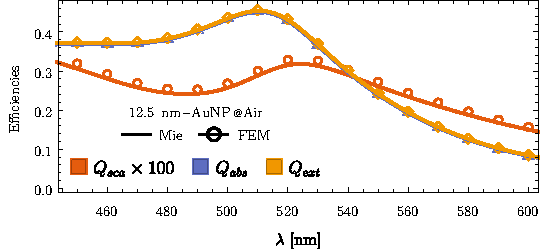
\includegraphics[width = .8\textwidth ]{1-Theory-Figs/Mie-FEM_Air.pdf}\\
%\includegraphics[width = .4\textwidth ]{1-Theory-Figs/Isolated-COMSOL.pdf}%
%\includegraphics[width = .4\textwidth ]{1-Theory-Figs/Isolated-COMSOL.pdf}%
%\caption[Convergence tests: The Meshing]{Resonance wavlength ($\lambda_\text{res}$) of the scattering (orange) and extinction (black) cross sections as functions of the NPs radii when embedded  \ref{sfig:red:1} into air and \ref{sfig:red:2} into water, and as function of the refractive index of the matrix for NP of radius set to  \ref{sfig:red:3} 12.5 nm and \ref{sfig:red:4} 50 nm.}
%\end{figure}




\begin{figure}[h!]\centering
	\def\svgwidth{.8\textwidth} \small
\includeinkscape{1-Theory-Figs/SistemaBox}
\vspace*{0em}
\caption[Spherical symmetric COMSOL Setup]{A 3D view (left) and the cross section (right) of a spherical symmetric COMSOL setup to calculate the optical response of a single spherical NP embedded into a matrix. The NP (yellow) is located at the center of the matrix (gray), which is covered by a PML layer (blue). The upper layer of the PML is hidden to allow a better view of the setup.}
\label{fig:setup:sphere}
\end{figure}

\begin{figure}[h!]
\def\svgwidth{\textwidth} \small
\hspace*{-1.25em}
\begin{subfigure}{.1\textwidth}\caption{ }\label{fig:Eff:sphere:First:a}\end{subfigure}
\vspace*{12.5em} % Crece la distancia entre as etiquetas
\\
\vspace*{-16.5em} % Crece la distancia entre las etiquetas y el pie de figura
\hspace*{-.75em}%
\begin{subfigure}{.1\textwidth}\caption{ }\label{fig:Eff:sphere:First:b}\end{subfigure}\\
\includeinkscape{1-Theory-Figs/4-Conv}
\vspace*{-1.5em} %Crece la ditancia entre la imagen y el pie de figura
\caption[Scattering, Absorption and Extinction Efficiencies of a 5 nm AuNP$@$Air: Analytical and FEM solutions with no optimizatio]{\textbf{a)} Scattering $Q_\text{sca}$, absorption $Q_\text{abs}$ and extinction $Q_\text{ext}$ efficiencies of a 5 nm AuNP embedded into air calculated by means of the Mie Theory (continuous) and the FEM (disks), and \textbf{b)} their absolute error, as function of the wavelength $\lambda$ of the incident planewave. The chosen parameters for the FEM calculations were based on the COMSOL Excercises \textbf{CITAR}.}
\label{fig:Eff:sphere:First}
\end{figure}


%

\chapter{Results and Discussion}
	\label{ch:Results}

    The problem of the absorption and scattering of light by a single nanoparticle (NP), illuminated by a monochromatic plane wave, is analytically described by the Mie Theory (Section \ref{s:Mie}) if the NP is considered to be embedded in an infinite medium (matrix). When more realistic conditions are considered, such as the presence of a second medium (substrate) forming a planar interface with the matrix and the possibility of a partial embedding of the NP inside the substrate, the Mie Theory is no longer be suited to study the optical properties of such systems. In this Chapter, the optical response of a gold (Au) spherical NP of radius $a = 12.5$ nm below, above and at a planar interface between air and glass is calculated through the Finite Element Method (FEM), when a monochromatic plane wave of wavelength $\lambda$ traveling in the direction $\vb{k}^\text{i}$ illuminates the system at an angle of incidence $\theta_i$ considering a defined polarization sate of the incident electric field $\vb{E}^\text{i}$. In order to identify the effect of the substrate and the embedding of the NPs inside the substrate, the absorption and scattering  efficiencies [Eqs. \eqref{eq:Csca}, \eqref{eq:Cabs} and \eqref{eq:Efficiencies}], as well the the radiation pattern (see Fig. \ref{fig:ScatteringMaps}) and the distribution of the induced electric field on and inside the NP (see Fig. \ref{fig:NearField}) are calculated numerically for the desired geometries and compared with limiting cases of the Mie theory: a AuNP isolated in a matrix of air and in a matrix of glass.

    The aforementioned analysis is organized as follows: In Section \ref{s:Totally} it is addressed the extreme cases of the supported and the totally embedded NP illuminated at normal incidence (Section \ref{s:Totally:Normal}) and at oblique incidence (Section \ref{s:TIR}), while in Section \ref{s:Emb} the effect of the partially embedding is studied considering once again  normal (Section \ref{s:Emb:Normal}) and oblique (Section \ref{s:Emb:Obl}) incidence.

    \section{Supported and Totally Embedded Spherical Particles}
     \label{s:Totally}
        % !TeX root = ../tesis.tex

To compare the optical response of a NP in the presence of a substrate with that of a NP in a totally homogeneous environment, let us first analyze the spectral response given by the Mie Theory when the matrix and the size of the NP varies. In Fig. \ref{fig:Mie:redshift} it is shown the wavelength of resonance $\lambda_\text{res}$, that is, the wavelength at which the scattering (orange) and extinction (black) efficiencies are maximized,  as a  function of the radius $a$ of a AuNP embedded in a matrix of air [Fig. \ref{sfig:red:1}] and of glass [Fig. \ref{sfig:red:2}], with a refractive index of $n_\text{m} = 1$ and $n_\text{m} = 1.5$, respectively, and as a function of the refractive index of the matrix $n_\text{m}$ for a AuNP with a radius of {$a = 12.5$ nm} [Fig. \ref{sfig:red:3}] and with a radius of $a = 50$ nm [Fig. \ref{sfig:red:4}]. For the optical response of the AuNP it was employed the experimental data as reported (filled circles) by \citeauthor{johnson_optical_1972} \cite{johnson_optical_1972}  and by considering a size correction ---see Appendix \ref{app:SizeCorrection}--- to it (empty circles).

\begin{figure}[h!] \centering
    \def\svgwidth{.9\textwidth}
    \includeinkscape[pretex = \small]{Redshift/redshift}
    \vspace*{-18.6em} \\
    \hspace*{-5.9em}%
        \begin{subfigure}{.20\textwidth}\caption{ }\label{sfig:red:1}\end{subfigure}%
        \begin{subfigure}{.235\textwidth}\caption{ }\label{sfig:red:2}\end{subfigure}%
        \begin{subfigure}{.20\textwidth}\caption{ }\label{sfig:red:3}\end{subfigure}%
        \begin{subfigure}{.24\textwidth}\caption{ }\label{sfig:red:4}\end{subfigure}
    \vspace*{16.5em}\\
    \caption[Spectral redshift of the scattering and extinction  efficiencies of a spherical AuNP as a function of its size and the embedding media]{Resonance wavelength $\lambda_\text{res}$ of the scattering (orange) and extinction (black) efficiencies of a AuNP as a function of the NP's radius when embedded \textbf{a)} in air ($n_\text{m} = 1)$ and \textbf{b)} in glass ($n_\text{m} = 1.5$), and as a function of the refractive index of the matrix  $n_\text{m}$ for a AuNP of radius \textbf{c)} 12.5 nm and \textbf{d)} 50 nm, using the dielectric function for gold as reported by \citeauthor{johnson_optical_1972} (filled circle) and considering a size correction to it (empty circles).}
    \label{fig:Mie:redshift}
\end{figure}

\textcolor{red}{
From the results shown in Fig. \ref{fig:Mie:redshift} it can be seen that, in general, the wavelength of resonance  $\lambda_\text{res}$ for the extinction is smaller than for the scattering  and that the distance between them decreases as either the size of the AuNP or the refractive index of the matrix increases, meaning that the contribution of the scattering to the extinction of light becomes larger alongside these parameters, as discussed in Section \ref{ss:AuMie}. An increase in $a$ or in $n_\text{m}$ diminishes the difference between the results with and without a size correction, as shown in Figs. \ref{sfig:red:1}, \ref{sfig:red:2} and \ref{sfig:red:4},  however if these results are contrasted  it can be noted on the one hand that the resonance wavelength only redshifts as $a$ grows when no size correction is considered (filled cirlces) but that a size corrected dielectric function (empty circles) give rise to a blueshift of $\lambda_\text{res}$ for values of radius $\lessapprox 15/n_\text{m}$ as seen if Figs. \ref{sfig:red:1} and \ref{sfig:red:2}. On the other hand, an increase in $n_\text{m}$ for a fixed radius presents only redshifts either with or without a size corrected dielectric function [see Fig. \ref{sfig:red:3}].
}

The spectral behavior of the scattering and extinction of light due to a spherical NP summarized in Fig. \ref{fig:Mie:redshift} was calculated by assuming a homogeneous medium (the matrix) embedding the NP and thus allowing the direction of the illuminating plane wave to be arbitrary, yet yielding the same results. In the following sections, the homogeneity of the surroundings of the NP is substituted by two semiinfinite media and thus modifying the optical response of the system depending on how it is illuminated.


        \subsection{Normal Incidence}
        % !TeX root = ../tesis.tex

The problem of scattering and absorption of light by single spherical NP embedded in a matrix, with refractive index $n_\text{m}$, illuminated by a plane wave with wavelength $\lambda$  and traveling in the  $\vb{k}^\text{i}$ direction, has spherical symmetry, which was exploited to develop the Mie Theory as explained in Section \ref{s:Mie}. If a substrate, with refractive index $n_\text{s}$, is considered and the NP is located right above or below the interface ---without crossing the substrate-matrix interface---, there are four combinations into which the system can be found since the NP can be either embedded  in the substrate or supported on it, and it can be illuminated either in an external ---from the matrix to the substrate--- or an internal ---from the substrate to matrix--- configuration, as shown in Fig. \ref{sfig:TotallyNormal:1}, where the following cases are depicted: Embedded-External (EE), Embedded-Internal (EI), Supported-External (SE) and Supported-Internal (SI). In the  presence of the substrate, the electric field illuminating the AuNP is not the incoming plane wave but the sum of it with the reflected electric field (EI and SE) or the transmitted electric field (EE and SI), both of which can be calculated analytically through Fresnel's reflection and transmission amplitude coefficients, as discussed in Appendix \ref{app:COMSOL}.

\begin{figure}[b!]
    \small
    \centering
    \hspace*{-.75\textwidth}%
        \begin{subfigure}{.37\textwidth}\caption{ }\label{sfig:TotallyNormal:1}\end{subfigure}%
        \begin{subfigure}{.25\textwidth}\caption{ }\label{sfig:TotallyNormal:2}\end{subfigure} \\[6em]
    \hspace*{-.38\textwidth}%
        \begin{subfigure}{.25\textwidth}\caption{ }\label{sfig:TotallyNormal:3}\end{subfigure} \\[-9em]
    \def\svgwidth{.95\textwidth}
    \includeinkscape{1-Totally/1-Efficiencies/1-Normal-Eff}%
    \vspace*{0em}
    \caption[Absorption and Scattering Efficiencies of a 12.5 nm AuNP above and below a planar Interface Illuminated at Normal Incidence]{\textbf{a)} Schematics of a AuNP embedded (E) in [supported (S) on] a glass substrate ($n_\text{s} = 1.5$) forming a planar interface with an air matrix ($n_\text{m} = 1$) and illuminated by a plane wave traveling normally to the air-glass interface in an external (E) and in an internal (I) configuration. \textbf{b)} Absorption $Q_\text{abs}$ and \textbf{c)} scattering $Q_\text{sca}$ efficiencies of a $12.5$ nm AuNP as a function of the wavelength $\lambda$ of the illuminating plane wave in different spatial configurations: EE (black), EI (orange), SE (blue) and SI (light orange). The green shaded region shows the two Mie-limiting cases of a  AuNP embedded in air and in glass; the magenta (AuNP and substrate) and cyan (Mie-limiting) markers correspond to the efficiencies evaluated at the wavelength of resonance for each case.
    }
\label{fig:TotallyNormal}
\end{figure}

In Figs. \ref{sfig:TotallyNormal:2} and \ref{sfig:TotallyNormal:3}  the absorption $Q_\text{abs}$ and scattering $Q_\text{sca}$ efficiencies are shown, respectively, as function of $\lambda$ for a AuNP of radius $a = 12.5$ nm in the Embedded-External (black), Embedded-Internal (orange), Supported-External (blue) and Supported-Internal (light orange) configurations; the green shaded areas correspond to the values between the two limiting cases given by the Mie theory: the AuNP embedded in air (lower boundary) and embedded in glass (upper boundary). The magenta markers correspond to the values of the efficiencies evaluated at the wavelength of resonance considering the presence of a substrate while the red markers correspond to the efficiencies at the resonance wavelength for the Mie-limiting cases.

From the results shown in Figs. \ref{sfig:TotallyNormal:2} and \ref{sfig:TotallyNormal:3}, it can be seen that both the absorption and scattering efficiencies of the four spatial configurations with substrate are of the same order of magnitud as the Mie-limiting cases and, even more, the nominal values of the efficiencies for the embedded AuNP (black and orange lines) lie very close to the Mie-limiting case of the AuNP in glass (upper boundary of the green shaded region) and the same behavior is observed for the supported AuNP (blue and light orange lines) and the Mie-limiting case of a AuNP embedded in air (lower boundary of the green shaded region). The presence of a substrate yields an overall enhancement and damping of the scattering and the absorption efficiencies relative to the isolated NP, which depend on the illumination of the system since $Q_\text{abs}$ and $Q_\text{ext}$ are inversely proportional to the refractive index of the medium of incidence [Ecs. \eqref{eq:Csca} and \eqref{eq:Cabs}]: If the system is illuminated in an external configuration, the obtained efficiencies are slightly decreased relative to the Mie-limiting case as it can be seen from the black  and blue curves, which correspond to the EE and SE cases; on the other hand, the calculated efficiencies for the internal illuminated cases, that is for EI (orange) and SI (light orange), are enhanced relative to the Mie-limiting cases.

Another effect of the substrate in the optical response of the system is a slightly spectral shift of the excitation wavelength of the scattering and absorption efficiencies, which depends on the medium where the AuNP is located. For example, in Figs. \ref{sfig:TotallyNormal:2} and \ref{sfig:TotallyNormal:3} the wavelength of resonance for both the absorption and the scattering efficiencies (magenta markers)  are redshifted $\sim 1$ nm, relative to the Mie-limiting case (cyan markers), for the AuNP supported on the substrate (blue and light orange curves) and blueshifted $\sim 2$ nm for the embedded AuNP (black and orange curves). \textcolor{red}{These spectral shifts can be understood by considering the AuNPs as point electric dipoles parallel to the interface ---an assumption consistent with the near-field distribution in the Mie-limiting cases and with the radiation patterns (see Figs.  \ref{fig:ScatteringMaps} and \ref{fig:NearField})--- and their interaction with the image point dipoles that are simultaneously induced within the substrate \cite{meng_anisotropic_2015}}. Both the dipoles induced in the AuNP and the image dipoles are parallel to the interface but its strength differs by  a factor of $A_\text{dip} = (\sqrt{n_j}-\sqrt{n_i}) / (\sqrt{n_j}+\sqrt{n_i})$ \cite{barrera1991optical}, where $n_{j}$ is the refractive index of the medium where the real dipole (the AuNP) is located and $n_i$ of the medium where the image dipole is induced. If the AuNP is embedded in the substrate, then $A_\text{dip}>0$ meaning that the induced dipole is parallel to the real dipole, which is a more energetic configuration that yields the spectral blueshift of the resonance. Contrarily, if the AuNP is supported on the substrate then $A_\text{dip}<0$ and the induced dipole is antiparallel to the real dipole, leading to a less energetic configuration and to the redshift observed in Figs. \ref{sfig:TotallyNormal:2} and \ref{sfig:TotallyNormal:3}.%
\index{Dipole!Image!Strength}

The absorption and scattering efficiencies are integral quantities which describe the global behavior of the induced electric field $\vb{E}^\text{ind}$, which corresponds to the internal electric field $\vb{E}^\text{int}$ inside the AuNP and to the scattered electric field $\vb{E}^\text{sca}$ outside of it. The distribution of $\vb{E}^\text{ind}$, for a fixed wavelength, is studied in two spatial regimes: the far- and the near-field. To analyze the optical response in the first regime, the radiation patterns of the AuNP are obtained numerically by plotting the norm of the scattered electric field in the far-field regime\footnote{\label{fnote:Stratton:Chu}%
    The FEM returns the induced electric field by a scatterer in a neighborhood around it  and there is no guarantee that the returned electric field, even at the boundaries of the volume where the FEM simulation is performed, corresponds to the far-field regime.  To calculate the radiation pattern from the obtained induced electric field, COMSOL Multiphysics\texttrademark{} Ver. 5.4  employs the  Stratton-Chu formula \cite{comsol_wave}, which is a near-field to far-field  transformation that  propagates the known electric near-field  over a mathematical surface surrounding all the scatterers  to an arbitrary point \cite{anyutin_algorithm_2019}. The Stratton-Chu formula is obtained by employing the vectorial generalization of the Green's second identity with the electric and magnetic near-fields and the Green's function to the scalar Helmholtz equation multiplied by a normal vector to the integration surface \cite{stratton_diffraction_1939}.%
}%
 $\vb{E}^\text{sca}_\text{far}$ as a function of the the angle relative to the normal direction to the interface. In Figs. \ref{fig:Far:Emb:Norm} and  \ref{fig:Far:Sup:Norm}, it is shown the radiation patterns of the embedded and the supported AuNP, respectively, for several values of the wavelength $\lambda$ of the incident plane wave, as well as considering an illumination of the system in an  [\textbf{a)} and \textbf{b})] external and in an  [\textbf{c)} and \textbf{d})] internal configuration; additionally, it is considered that the incident electric field is totally [\textbf{a)} and \textbf{c})] parallel to the scattering plane $\vb{E}^\text{i}_\parallel$ and [\textbf{b)} and \textbf{d})] perpendicular to the scattering plane $\vb{E}^\text{i}_\perp$.

\begin{figure}[b!]
    \centering
    \def\svgwidth{.8\textwidth}
    \hspace*{-.215\textwidth}%
    \vspace*{-.5em}%
        \begin{subfigure}{.32\textwidth}\caption{\footnotesize$\dfrac{\norm{\vb{E}^\text{sca}_\text{far}}}{\norm{\vb{E}^\text{i}}} \times 10^{-9}$  }\label{sfig:Far:Emb:Norm:a}\end{subfigure}%
        \begin{subfigure}{.4\textwidth}\caption{\footnotesize$\dfrac{\norm{\vb{E}^\text{sca}_\text{far}}}{\norm{\vb{E}^\text{i}}} \times 10^{-9}$  }\label{sfig:Far:Emb:Norm:b}\end{subfigure}\\
    \includeinkscape[pretex = \footnotesize]{1-Totally/4-5-Far-XY-Embedded/4-5-Far-XY-Embedded-External}\\
    %
    \def\svgwidth{.8\textwidth}
    \hspace*{-.215\textwidth}%
    \vspace*{-.5em}%
        \begin{subfigure}{.32\textwidth}\caption{\footnotesize$\dfrac{\norm{\vb{E}^\text{sca}_\text{far}}}{\norm{\vb{E}^\text{i}}} \times 10^{-9}$  }\label{sfig:Far:Emb:Norm:c}\end{subfigure}%
        \begin{subfigure}{.4\textwidth}\caption{\footnotesize$\dfrac{\norm{\vb{E}^\text{sca}_\text{far}}}{\norm{\vb{E}^\text{i}}} \times 10^{-9}$  }\label{sfig:Far:Emb:Norm:d}\end{subfigure}\\
    \includeinkscape[pretex = \footnotesize]{1-Totally/4-5-Far-XY-Embedded/4-5-Far-XY-Embedded-Internal}%
    \caption[ Radiation pattern of a AuNP totally embedded in a substrate illuminated at normal incidence ]{Radiation patterns of a AuNP (light yellow) of radius $a = 12.5$ nm, embedded in a substrate (light blue) and illuminated by an electric plane wave $\vb{E}^\text{i}$ with a wavelength $\lambda$, traveling in the $\vb{k}^\text{i}$ direction normal to the interface between the substrate ($n_\text{s} = 1.5$) and the matrix ($n_\text{m} = 1)$. The radiation patterns consider the illumination of the system  \textbf{a,b)} in an external and  \textbf{c,d)} in an internal configuration, and with an incident electric field \textbf{a,c)}  $\vb{E}^\text{i}_\parallel$ parallel to the scattering plane and \textbf{b,d)} $\vb{E}^\text{i}_\perp$ perpendicular to it.}
    \label{fig:Far:Emb:Norm}
\end{figure}

The radiation patterns of both the embedded  and the supported AuNP follow the same trend independently of the illuminating wavelength $\lambda$ but the amplitude is modulated by the scattering efficiencies shown in Fig. \ref{sfig:TotallyNormal:3}. For example, in the EE  and EI cases (Fig. \ref{fig:Far:Emb:Norm}) the scattered electric field (in the far-field) decreases its amplitude as the wavelength increases from $400$ nm to $480$ nm (black, orange and blue curves) and from   $550$ nm to $600$  nm, while it increases from $485$ nm to $542$ nm, near the wavelength of resonance for the scattering efficiency, see Fig. \ref{sfig:TotallyNormal:3}. Similarly, for the SE and SI  the amplitude of the far-field is modulated by its scattering efficiency as it can be seen from comparing the radiation patterns in Fig. \ref{fig:Far:Sup:Norm} at $400$ mn (black), $480$ nm (blue) and  $527$ nm (purple), with the value of $Q_\text{sca}$ at those wavelengths  corresponding to a global maximum, a global minimum and a local maximum at the wavelength of resonance, respectively [see Fig. \ref{sfig:TotallyNormal:3}].

\begin{figure}[t!]
    \centering
    \def\svgwidth{.8\textwidth}
    \hspace*{-.215\textwidth}%
    \vspace*{-.5em}%
        \begin{subfigure}{.32\textwidth}\caption{\footnotesize$\dfrac{\norm{\vb{E}^\text{sca}_\text{far}}}{\norm{\vb{E}^\text{i}}} \times 10^{-9}$  }\label{sfig:Far:Sup:Norm:a}\end{subfigure}%
        \begin{subfigure}{.4\textwidth}\caption{\footnotesize$\dfrac{\norm{\vb{E}^\text{sca}_\text{far}}}{\norm{\vb{E}^\text{i}}} \times 10^{-9}$  }\label{sfig:Far:Sup:Norm:b}\end{subfigure}\\
    \includeinkscape[pretex = \footnotesize]{1-Totally/4-5-Far-XY-Supported/4-5-Far-XY-Supported-External}\\
    %
    \def\svgwidth{.8\textwidth}
    \hspace*{-.215\textwidth}%
    \vspace*{-.5em}%
        \begin{subfigure}{.32\textwidth}\caption{\footnotesize$\dfrac{\norm{\vb{E}^\text{sca}_\text{far}}}{\norm{\vb{E}^\text{i}}} \times 10^{-9}$  }\label{sfig:Far:Sup:Norm:c}\end{subfigure}%
        \begin{subfigure}{.4\textwidth}\caption{\footnotesize$\dfrac{\norm{\vb{E}^\text{sca}_\text{far}}}{\norm{\vb{E}^\text{i}}} \times 10^{-9}$  }\label{sfig:Far:Sup:Norm:d}\end{subfigure}\\
    \includeinkscape[pretex = \footnotesize]{1-Totally/4-5-Far-XY-Supported/4-5-Far-XY-Supported-Internal}%
    \caption[  Radiation pattern of a AuNP supported into a substrate illuminated at normal incidence ]{Radiation patterns of a AuNP (light yellow) of radius $a = 12.5$ nm, supported on a substrate (light blue) and illuminated by an electric plane wave $\vb{E}^\text{i}$ with a wavelength $\lambda$, traveling in the $\vb{k}^\text{i}$ direction normal to the interface between the substrate ($n_\text{s} = 1.5$) and the matrix ($n_\text{m} = 1)$. The radiation patterns consider the illumination of the system  \textbf{a,b)} in an external and  \textbf{c,d)} in an internal configuration, and with an incident electric field \textbf{a,c)}  $\vb{E}^\text{i}_\parallel$ parallel to the scattering plane and \textbf{b,d)} $\vb{E}^\text{i}_\perp$ perpendicular to it.}
    \label{fig:Far:Sup:Norm}
\end{figure}

The shape of the radiation pattern of a 12.5 nm AuNP in the presence of a substrate, either embedded or supported, resembles that of the isolated 12.5 AuNP discussed in Section \ref{sss:FarField} [see Fig. \ref{fig:ScatteringMaps}] in that it follows a two-lobe and a one-lobe pattern depending on the orientation of $\vb{E}^\text{i}$ relative to the scattering plane. If the incident electric field is parallel to the scattering plane, a two-lobe pattern aligned to the direction $\vb{k}^\text{i}$ of the incident ---and transmitted--- plane wave arises as it can be seen in the Figs. \ref{sfig:Far:Emb:Norm:a} and  \ref{sfig:Far:Emb:Norm:c} for the EE case, and Figs.  \ref{sfig:Far:Sup:Norm:a} and \ref{sfig:Far:Sup:Norm:c} for the EI scenario. Contrastingly, when the incident electric field is perpendicular to the scattering plane, the one-lobe pattern can be identified [see Figs. \ref{sfig:Far:Emb:Norm:b} and \ref{sfig:Far:Emb:Norm:d} (SE), and \ref{sfig:Far:Sup:Norm:b} and \ref{sfig:Far:Sup:Norm:d} (SI)]. By comparing the Mie-limiting radiation pattern (see Fig. \ref{fig:ScatteringMaps}), to the radiation patterns considering a substrate, the later loses the polar symmetry observed in the Mie-limiting case.  In particular, the amplitude of $\vb{E}^\text{sca}_\text{far}$ is larger when evaluated at the medium of incidence  than at medium of transmission; this asymmetry is observed for both illuminating configurations (external and internal) and it does not depend on whether the AuNP is supported or embedded. Rather, the spatial configuration of the system determines the overall value of the far-field: when the AuNP is embedded, the far-field amplitude is greater by a factor of $2.5$  than when the AuNP is supported ---see the axis scale in Figs. \ref{fig:Far:Emb:Norm} and \ref{fig:Far:Sup:Norm}---; this phenomenon  is a consequence of the two following physical mechanisms. The first is the substrate having a greater refractive index than the matrix, thus making the optical response of the 12.5 nm AuNP as that of a larger NP ---but still small compared to the illuminating wavelength---, as in the Mie-limiting case. The second mechanism is the relative alignment of a point dipole ---small particle approximation to the AuNP--- and the induced dipole due to the interface, which is parallel when the AuNP is embedded onto the substrate and antiparallel when supported on it, thus leading to a more energetic configuration when the AuNP is located inside the substrate than inside the matrix.

The radiation pattern, an optical property observed in the far-field regime, is a manifestation of the near-field spatial distribution ---see the footnote on page \pageref{fnote:Stratton:Chu}--- which can be calculated numerically through the FEM for a AuNP of radius $a = 12.5$ nm. The scattered electric field in the  far-field regime of a AuNP embedded or supported  [Figs. \ref{fig:Far:Emb:Norm} and \ref{fig:Far:Sup:Norm}] share some characteristic to the radiated field of an isolated AuNP (Mie-limiting case), and thus should the near-field. In Fig. \ref{fig:Near:IntExt} it is shown the module of the induced electric field $\vb{E}^\text{ind}$ when the AuNP is illuminated by a $y$-polarized incident electric field $\vb{E}^\text{i}$ traveling in the $\vb{k}^\text{i}$ direction, perpendicular to the interface between air and glass; the induced electric field is evaluated at the scattering plane $x = 0$, that is, the incident electric field has only a parallel contribution $\vb{E}^\text{i}_\parallel$ to the scattering plane. The wavelength $\lambda$ of the incoming plane wave is $\lambda =535.2$ nm for an embedded AuNP either illuminated externally [Fig.  \ref{sfig:Near:EE}] or internally  [Fig.  \ref{sfig:Near:EI}] and  $\lambda =510$ nm for a supported AuNP either illuminated externally [Fig.  \ref{sfig:Near:SE}] or internally  [Fig.  \ref{sfig:Near:SI}], which correspond to the wavelengths of the Localized Surface Plasmon Resonance (LSPR).

\begin{figure}[t!]\centering
   \def\svgwidth{.75 \textwidth}
   \footnotesize
   \captionsetup[subfigure]{labelfont ={normal,bf,color = white}}
   \includeinkscape{1-Totally/2-NearY/2-NearY-EmbSup}\\[-32.6em]
   \hspace*{-.25\textwidth}
       \begin{subfigure}{.25\textwidth}\caption{ } \label{sfig:Near:EE}\end{subfigure}%
       \begin{subfigure}{.36\textwidth}\caption{ } \label{sfig:Near:EI}\end{subfigure}\\[13em]
   \hspace*{-.25\textwidth}
       \begin{subfigure}{.25\textwidth}\caption{ } \label{sfig:Near:SE}\end{subfigure}%
       \begin{subfigure}{.36\textwidth}\caption{ } \label{sfig:Near:SI}\end{subfigure}\\[15em]
   \caption[Induced Electric Field of a 12.5 nm Au Spherical NP embbeded into (supported on) a substrate illuminated at a normal incidence]{Magnitude of the electric field induced $\vb{E}^\text{ind}$ by a 12.5 nm AuNP   (dashed black lines) illuminated by an incident electric plane wave $\vb{E}^\text{i}$ traveling in the $\vb{k}^\text{i}$ direction perpendicular to the interface  (dashed white lines) between an air matrix ($n_\text{m} = 1$) and a glass substrate ($n_\text{s} = 1.5$) when the AuNP is  \textbf{a,b)} embedded in the glass substrate and \textbf{c,d)} supported on it; the system is illuminated \textbf{a,c)}  in an external and \textbf{b,d)} in an internal configuration at the resonance wavelength for the absorption efficiency.}
   \label{fig:Near:IntExt}
 \end{figure}

The spatial distribution of the near-field, shown in Fig. \ref{fig:Near:IntExt}, is consistent with the description and explanation of both the absorption and scattering efficiencies [Fig. \ref{sfig:TotallyNormal:2}] and the radiation patterns of the embedded [Fig. \ref{fig:Far:Emb:Norm}] and the supported [Fig. \ref{fig:Far:Sup:Norm}] AuNP. The induced electric field is in general, stronger when the AuNP is embedded in the substrate than when it is supported on it, as it can be seen in the value of the hotspots around the AuNP: reddish regions in Figs. \ref{sfig:Near:EE} and \ref{sfig:Near:EI} and bluish in Figs. \ref{sfig:Near:SE} and \ref{sfig:Near:SI}. These hotspots also verifies that at the resonance wavelength, the main contribution to the electric fields is due to an electric dipolar moment since the characteristic two-lobe distribution of the near-field can be easily identified nevertheless, the lobes are not horizontally aligned to the AuNP's equator but farther from the substrate for the embedded AuNP and closer to it for the supported AuNP, as if the induced dipole ---in the small particle approximation, where the AuNP is treated as a point electric dipole--- is parallel (perpendicular) to the dipolar moment induced in the AuNP when it is embedded in (supported on) the substrate, as discussed above.

Throughout this section, it was studied the optical properties of a 12.5 nm AuNP on the presence of a substrate considering four configurations: the AuNP either embedded or supported and the system illuminated from under the substrate or from above. The choice of normal incidence to the system allowed the obtained results to be compared with the Mie-limiting case, which lead to the identification of similarities and differences among the four configurations. The differences in the optical response are associated to the broken symmetry due to the two semiinfinte media now considered \cite{meng_anisotropic_2015}, while the similarities arise since the system is always illuminated by a plane wave independently of the choice of the medium of incidence, yielding a mostly dipolar electric field. Therefore, in the next section the oblique incidence case is addressed only when the AuNP is supported and illuminated in the internal configuration since it is the only case with a different illumination to the system: an evanescent wave for incidence angles above the critical angle $\theta_c =\arcsin(n_\text{m}/n_\text{s})$ \cite{born_max_principle_1999}.

         \label{s:Totally:Normal}
         
         \subsection{Supported Spherical Particle in Total Internal Reflection}
         \label{s:TIR}
         % !TeX root = ../tesis.tex

In the past section, the AuNP of radius $a = 12.5$ nm was illuminated at normal incidence in four different spatial configurations considering the  presence of a substrate: the AuNP either embedded in the substrate (with a refractive index $n_\text{s}$) or supported on it embedded in an air matrix (with refractive index $n_\text{s}$), and the incident electric field  illuminating the system from the substrate (internal configuration) or from the matrix (external configuration). By considering that the incident electric plane wave $\vb{E}^\text{i}$  propagates from the substrate to the matrix at an angle $\theta_i$, relative to the normal direction to the interface between the two media, the electric field interacting with the AuNP is the transmitted field, that propagates at a transmission angle $\theta_t = \asin(n_\text{m}\sin\theta_i/n_\text{s})$ \cite{born_max_principle_1999} and two differences arises compared to the normal incidence cases: there are two different polarization states for $\vb{E}^\text{i}$ ---$s$ and $p$ polarization\footnote{%
    The $s$ and $p$ polarization states of the electric field are defined by considering its oscillations perpendicular and parallel, respectively, to the incidence plane, defined by the the propagating direction of the incident electric plane wave and the normal direction to the interface between the substrate and the matrix \cite{bohren_absorption_1983}.}%
--- and if $\theta_i$ is greater than the critical angle $\theta_c = \asin(n_\text{m}/n_\text{s})$ the transmitted electric field ceases to be a plane wave and it is now described by an evanescent wave propagating along the interface  \cite{born_max_principle_1999}. Similarly to the past section, the optical properties of the supported AuNP illuminated at an oblique incidence in an internal configuration are studied by analyzing the absorption and scattering efficiencies, the radiation pattern and, lastly, the induced electric field on the AuNP.

\begin{figure}[b!]
    \def\svgwidth{.95\textwidth}
    \centering
    \hspace*{-28.5em}%
    \vspace*{-1.25em}%
        \begin{subfigure}{.71\textwidth}\caption{ }\label{sfig:SuppObl:Eff:Abs}\end{subfigure}%
        \begin{subfigure}{.25\textwidth}\caption{ }\label{sfig:SuppObl:Eff:Sca}\end{subfigure} \\
    \includeinkscape[pretex = \small]{2-SuppObl/1-Efficiencies/1-Oblique-Supp-Eff}%
    \vspace*{-.5em}
    \caption[Absorption and Scattering Efficiencies of a 12.5 nm AuNP on a Interface Illuminated in an internal configuration at oblique incidence]{\textbf{a)} Absorption and \textbf{b)} scattering efficiencies of a $12.5$ nm AuNP in an air matrix ($n_\text{m} = 1$) and supported on a glass substrate ($n_\text{s} = 1.5$) as function of the wavelength $\lambda$ of an  $s$ (filled circle/solid lines) and a $p$ (empty circle/dashed lines) polarized incident electric plane wave propagating in the direction of the wave vector $\vb{k}^\text{i}$, in an internal configuration, at an angle of incidence $\theta_i$ of $15^\circ$ (black),  $38^\circ$ (orange),  $42^\circ$ (blue) and  $75^\circ$ (light orange) relative to the normal direction to the glass-air interface. The green shaded region shows the two Mie-limiting cases of a AuNP embedded in air and in glass; the magenta (supported AuNP) and red (Mie-limiting) markers corresponds to the efficiencies evaluated at the wavelength of resonance for each case.}
\label{fig:SuppObl:Eff}
\end{figure}

In Fig. \ref{fig:SuppObl:Eff} the absorption $Q_\text{abs}$ [Fig.\ref{sfig:SuppObl:Eff:Abs}] and scattering $Q_\text{sca}$ [Fig. \ref{sfig:SuppObl:Eff:Sca}] efficiencies of a 12.5 nm AuNP in air ($n_\text{m} = 1$) supported on a glass substrate ($n_\text{s} = 1.5$) are shown as function of the wavelength $\lambda$ of the incident electric field $\vb{E}^\text{i}$ illuminating the AuNP from the substrate at an incidence angle $\theta_i$ of $15^\circ$ (black),  $38^\circ$ (orange),   $42^\circ$ (blue) and  $75^\circ$ (light orange) considering an $s$ (filled circle/solid lines) and a $p$ (empty circle/dashed lines) polarization for $\vb{E}^\text{i}$. Since the critical angle for a glass-air interface is $\theta_c = 41.8^\circ$, the blue and light orange curves show the results of the interaction between an evanescent wave and the AuNP. The magenta markers correspond to the values of $Q_\text{abs}$ and $Q_\text{sca}$ evaluated at the wavelength of resonance; the Mie-limiting cases (AuNP embedded in air and in glass)  are signalized by the boundaries of the green shaded region  and the red markers correspond to the resonances of their efficiencies.

A general behavior on both the absorption and scattering efficiencies is that their value for all considered values of $\lambda$, with a fixed polarization state, increases as the angle of incidence reaches the critical angle $41.8^\circ$ as it can be seen by comparing the black, orange ---$\theta_i = 15^\circ,\, 38^\circ < \theta_c$---  and blue ---$\theta_c<\theta_i = 42^\circ$--- curves, and they decrease in the interval  $\theta_c<\theta_i<90^\circ$, which it it noticeable by comparing the aforementioned curves with the light orange one ---$\theta_i = 75^\circ$---. This tendency on the overall value of $Q_\text{abs}$ and $Q_\text{abs}$ is due to the transmitted electric field which illuminates the AuNP and it is described by a plane wave for $\theta_i<\theta_c$ and by an evanescent wave for $\theta_i>\theta_c$ accoriding to the Fresnel's transmission amplitude coefficients \textcolor{red}{\textbf{Sería buena idea ponerlas en el apéndice de COMSOL?}}, whose real part are monotonically increasing (decreasing) functions of $\theta_i$ for values smaller (greater) to the critical angle. Yet, another explanation for the decreasing behavior after the critical angle is due to the penetration depth of the evanescent electric field, which is given by $\lambda/(2\pi n_\text{s}\sin\theta_i)$, meaning that evanescent wave penetrates deeper into the matrix for values of $\theta_i$ above and near $\theta_c$ leading to a stringer interaction with the AuNP.

When comparing the absorption and scattering efficiencies based on the polarization of the incident plane wave, it can be observed that their enhancement, relative to the Mie-limiting case of a AuNP in a air matrix, is greater for a  \textit{p} than for an \textit{s} polarized incident electric field for a fixed angle of incidence (see continuos and dashed curves of the same color). Another notable phenomena is that the  efficiencies for $\theta_i=75^\circ$ (light orange curves)  are bellow the Mie-limiting case for all wavelengths, while only the efficiencies for  \text{p} polarized incident electric field with $\theta_i = 42^\circ \gtrsim \theta_c$ (dashed blue curves) are greater than the glass Mie-limiting case at the resonance wavelength. The last difference between the \textit{s} and the \textit{p} polarization cases arises by analyzing the spectral shift of the LSPR (magenta markers). For a fixed polarization state, all the LSPR are excited at the same wavelength independently of the angle of incidence up to the wavelength discretization ---$\Delta \lambda = 2.5$ nm in the LSPR's neighborhood --- employed in the FEM simulations from Fig. \ref{fig:SuppObl:Eff}: The absorption extinction wavelength for the \textit{s} polarized incident electric field is $\sim 510$ nm, which is the same as the equivalent system illuminated at normal incidence [see Fig. \ref{sfig:TotallyNormal:2}], while the LSPR for the $p$ polarization case is excited at the larger wavelength $\sim 512.5$ nm. To better understand the spectral shift between the two polarization states the induced electric field in the far and near-field regimes are analyzed.

The radiation pattern of the 12.5 nm AuNP embedded in air and supported on a glass substrate is shown in Fig. \ref{fig:Far:SuppObl} when an $s$ polarized [Figs. \ref{sfig:Far:SuppObl:s:a} and \ref{sfig:Far:SuppObl:s:b}] and a  $p$ polarized [Figs. \ref{sfig:Far:SuppObl:p:c} and \ref{sfig:Far:SuppObl:p:d}] incident electric field $\vb{E}^\text{i}$ illuminates the AuNP at an incidence angle of $\theta_i = 15^\circ$ (black) and $\theta_i = 38^\circ$ ---below the critical angle $\theta_c = 41.8^\circ$---, and $\theta_i = 42^\circ$ (black) and $\theta_i = 75^\circ$ ---above  $\theta_c$--- in an internal configuration at the wavelengths of resonance of the absorption efficiency ---magenta markers in Fig. \ref{sfig:SuppObl:Eff:Abs}--- for each case, which corresponds to the LSPR. The scattering plane where the radiation pattern is shown in Figs. \ref{sfig:Far:SuppObl:s:a} and \ref{sfig:Far:SuppObl:p:c}  is perpendicular to the incidence plane (vertical gray dotted lines) while the scattering plane overlaps the incidence plane in Figs. \ref{sfig:Far:SuppObl:s:b} and \ref{sfig:Far:SuppObl:p:d}; the incident wave vector $\vb{k}^\text{i}$ and the components of the incident electric field parallel $\vb{E}^\text{i}_\parallel$ and perpendicular $\vb{E}^\text{i}_\perp$ to the scattering plane are schematized in all cases.

\begin{figure}[t!]
    \centering
    \def\svgwidth{.8\textwidth}
    \hspace*{-.215\textwidth}%
    \vspace*{-.5em}%
        \begin{subfigure}{.32\textwidth}\caption{\footnotesize$\dfrac{\norm{\vb{E}^\text{sca}_\text{far}}}{\norm{\vb{E}^\text{i}}} \times 10^{-9}$  }\label{sfig:Far:SuppObl:s:a}\end{subfigure}%
        \begin{subfigure}{.4\textwidth}\caption{\footnotesize$\dfrac{\norm{\vb{E}^\text{sca}_\text{far}}}{\norm{\vb{E}^\text{i}}} \times 10^{-9}$  }\label{sfig:Far:SuppObl:s:b}\end{subfigure}\\
    \includeinkscape[pretex = \footnotesize]{2-SuppObl/4-5-FarXY/4-5-Far-XY-S}\\
    %
    \def\svgwidth{.8\textwidth}
    \hspace*{-.215\textwidth}%
    \vspace*{-.5em}%
        \begin{subfigure}{.32\textwidth}\caption{\footnotesize$\dfrac{\norm{\vb{E}^\text{sca}_\text{far}}}{\norm{\vb{E}^\text{i}}} \times 10^{-9}$  }\label{sfig:Far:SuppObl:p:c}\end{subfigure}%
        \begin{subfigure}{.4\textwidth}\caption{\footnotesize$\dfrac{\norm{\vb{E}^\text{sca}_\text{far}}}{\norm{\vb{E}^\text{i}}} \times 10^{-9}$  }\label{sfig:Far:SuppObl:p:d}\end{subfigure}\\
    \includeinkscape[pretex = \footnotesize]{2-SuppObl/4-5-FarXY/4-5-Far-XY-P}%
    \caption[  Radiation pattern of a AuNP supported on a substrate illuminated at oblique incidence]{Radiation pattern of a AuNP (light yellow) of radius $a = 12.5$ nm supported on a glass substrate (light blue, $n_\text{s} = 1.5$) with an air matrix ($n_\text{m} = 1$) illuminated by an incident electric plane wave $\vb{E}^\text{i}$, with a wavelength $\lambda$, traveling in the $\vb{k}^\text{i}$ direction at an angle of incidence $\theta_i$ of $15^\circ$ (black),  $38^\circ$ (orange),  $42^\circ$ (blue) and  $75^\circ$ (light orange) relative to the normal direction to the glass-air interface. The radiation patterns consider an \textbf{a,b)} $s$ polarized and  a \textbf{c,d}) $p$ polarized incident electric field and the scattering plane \textbf{a,c)} perpendicular to the incidence plane (vertical gray dotted lines) and \textbf{b,d)} equal to the incidence plane. In all cases the incident wave vector $\vb{k}^\text{i}$, the perpendicular $\vb{E}_\perp^\text{i}$ and the  parallel $\vb{E}_\parallel^\text{i}$ projection of the incident electric field relative to the scattering plane are schematized.%
    }
    \label{fig:Far:SuppObl}
\end{figure}

As expected from the results in Section \ref{s:Totally:Normal}, the amplitudes of the radiation patterns for AuNP supported on a substrate and illuminated in an internal configuration at an oblique incidence are modulated by the absorption and scattering efficiencies, for example, the maximum value of the radiation pattern for the $s$ polarization case is $1.2 \text{ nV m}^{-1}$ [see Figs. \ref{sfig:Far:SuppObl:s:a} and \ref{sfig:Far:SuppObl:s:b}] while this value is two folded for the $p$ polarization case [see Figs. \ref{sfig:Far:SuppObl:p:c} and \ref{sfig:Far:SuppObl:p:d}]. Additionally, the radiation pattern is in average greater for a fixed angle of incidence, the greater the absorption and scattering efficiencies are, as it can be seen by comparing blue and the light orange curves ---corresponding to $\theta_i = 42^\circ$ and $\theta_i = 75^\circ$, respectively--- in Fig. \ref{fig:Far:SuppObl} with the curves in Fig. \ref{fig:SuppObl:Eff}.

If the shape of the radiation patterns is studied, the $s$ polarization case shows a two and a one-lobe shapes if the incident electric field is parallel [Fig. \ref{sfig:Far:SuppObl:s:a}] or perpendicular [Fig. \ref{sfig:Far:SuppObl:s:b}] to the scattering plane, respectively. Such radiation patterns are observed for all values of $\theta_i$ in an $s$ polarization configuration due to the continuity of the components of the electric field parallel the substrate where the the AuNP is onto. On the other hand, for a $p$ polarized incident electric field, the transmitted electric field illuminating the AuNP has a different component perpendicular to the substrate depending on the angle of incidence; the orientation of the transmitted electric field, relative to the normal direction to the substrate, is obtained by adding $-\pi/2$ to the angle of transmission $\theta_t = \arcsin(n_\text{m}\sin\theta_i/n_\text{s})$, that is $\theta_t - \pi/2$. The direction of the transmitted electric field for an incidence angle $\theta_i = 15^\circ<\theta_c$ and $\theta_i = 38^\circ<\theta_c$ ---black and orange curves--- result on the two-lobe shapes  in Fig. \ref{sfig:Far:SuppObl:p:c} ---scattering plane perpendicular to the incidence plane--- and Fig. \ref{sfig:Far:SuppObl:p:d} ---scattering plane overlapping the incidence plane---. When the scattering and incidence plane are perpendicular to each other, the transmitted electric field have components both parallel and perpendicular to the scattering plane for $\theta_i<\theta_c$ yielding radiation patterns without non-radiation directions, while the radiation patterns when the scattering and the incidence plane overlap are two-lob shapes rotated with no-radiation directions given by the transmission angle $\theta_t$. For $\theta_i>\theta_c$, the transmitted electric field is described by an evanescent wave traveling along the interface and its direction is perpendicular to the the substrate, thus the two-lobe shape of the AuNP's radiation pattern is aligned to the interface; this can be observed when $\theta_i = 42^\circ$ (blue curve) and $\theta_i = 75^\circ$ (light orange curve) when the scattering and the incidence plane are perpendicular between them [Fig. \ref{sfig:Far:SuppObl:p:c}] and when they overlap [Fig. \ref{sfig:Far:SuppObl:p:d}].

The behavior of the scattered electric field by the AuNP, in the far-field regime, described above suggests that a 12.5 nm AuNP on a substrate can be studied in the small particle approximation and be treated, even at oblique incidence, as a point dipole oriented  parallel to the substrate for an $s$ polarized incident electric field and in a perpendicular direction to that given by the transmission angle for the $p$ polarization case. Under such schema, alongside the interaction between the point dipole and an image dipole induced due to the substrate, the difference in magnitud of the efficiencies, and thus of the far-field, for different polarization states of the incident electric field  is understood since for $s$ polarization the point and the image dipole are parallel to each other, while for  $p$ polarization the dipoles are collinear to each other, that is, they have a stronger response \textcolor{red}{\bf Buscar referencia}.

To further analyze the optical response of the AuNP on a substrate, the spatial distribution of the induced electric field $\vb{E}^\text{ind}$ ---the internal and the scattered electric field in the near-field regime--- is needed. Since the radiation patterns observed when an $s$ polarized incident electric field illuminates the AuNP follow the same one and a two-lobe shapes for all the considered combinations of $\theta_i$ and $\lambda$ only differing on the magnitud, the distribution of $\vb{E}^\text{ind}$  have the same qualitative behavior for all incident angles at this polarization state. Therefore, the norm of the induced electric field $\norm{\vb{E}^\text{ind}}$, evaluated at a scattering plane perpendicular to the incidence plane (vertical gray dashed lines) is shown in Fig. \ref{fig:Near:SuppObl:s} for a 12.5 nm AuNP (black dashed lines) supported on the interface between a glass substrate and an air matrix (white dashed lines) when the incident electric field $\vb{E}^\text{i}$ illuminates the system at an incident angle of $15^\circ$ [Fig. \ref{sfig:Near:SuppObl:s:15}], $38^\circ$ [Fig. \ref{sfig:Near:SuppObl:s:38}], $42^\circ$ [Fig. \ref{sfig:Near:SuppObl:s:42}]  and $75^\circ$ [Fig. \ref{sfig:Near:SuppObl:s:75}].

\begin{figure}[t!]\centering
   \def\svgwidth{.75\textwidth}
   \footnotesize
   \captionsetup[subfigure]{labelfont ={normal,bf,color = white}}
   \includeinkscape{2-SuppObl/2-Near-sP/2-NearYX-sPol}\\[-32.6em]
   \hspace*{-.25\textwidth}
       \begin{subfigure}{.25\textwidth}\textcolor{red}{\caption{ } \label{sfig:Near:SuppObl:s:15}}\end{subfigure}%
       \begin{subfigure}{.34\textwidth}\caption{ }\label{sfig:Near:SuppObl:s:38}\end{subfigure}\\[13em]
    \hspace*{-.25\textwidth}
       \begin{subfigure}{.25\textwidth}\textcolor{red}{\caption{ } \label{sfig:Near:SuppObl:s:42}}\end{subfigure}%
       \begin{subfigure}{.34\textwidth}\caption{ }\label{sfig:Near:SuppObl:s:75}\end{subfigure}\\[15em]
\caption[Induced Electric Field of a 12.5 nm Au NP on substrate illuminated at oblique incidence with a $s$ polarized electric field]{%
Electric field $\vb{E}^\text{ind}$ induced by a supported 12.5 nm AuNP (dashed black lines) illuminated by an $s$ polarized incident electric plane wave $\vb{E}^\text{i}$ traveling in the $\vb{k}^\text{i}$ direction, in an internal configuration, at an angle of incidence of \textbf{a)} $15^\circ$, \textbf{b)} $38^\circ$, \textbf{c)} $42^\circ$ and \textbf{d)} $75^\circ$, relative to the normal direction to the interface ---white dashed lines--- between an air matrix ($n_\text{m} = 1$) and a glass substrate ($n_\text{s} = 1.5$). The incident electric plane wave is evaluated at $\lambda = 510$ nm ---resonance wavelength of the absorption efficiency--- and in all shown cases the scattering plane is perpendicular to the incidence plane (vertical gray dotted lines).
}
 \label{fig:Near:SuppObl:s}
 \end{figure}

 \begin{figure}[!h]\centering
    \def\svgwidth{.7\textwidth}
    \scriptsize
    \captionsetup[subfigure]{labelfont ={small,bf,color = white}}
    \includeinkscape{2-SuppObl/3-Near-pP/2-NearYX-pPol}\\[-62.75em]
    \hspace*{-.255\textwidth}
        \begin{subfigure}{.25\textwidth}\textcolor{red}{\caption{ } \label{sfig:Near:SuppObl:p:15:perp}}\end{subfigure}%
        \begin{subfigure}{.3\textwidth}\caption{ }\label{sfig:Near:SuppObl:p:15:par}\end{subfigure}\\[12.8em]
    \hspace*{-.225\textwidth}
        \begin{subfigure}{.225\textwidth}\textcolor{red}{\caption{ } \label{sfig:Near:SuppObl:p:38:perp}}\end{subfigure}%
        \begin{subfigure}{.34\textwidth}\caption{ }\label{sfig:Near:SuppObl:p:38:par}\end{subfigure}\\[12.8em]
    \hspace*{-.225\textwidth}
        \begin{subfigure}{.225\textwidth}\textcolor{red}{\caption{ } \label{sfig:Near:SuppObl:p:42:perp}}\end{subfigure}%
        \begin{subfigure}{.34\textwidth}\caption{ }\label{sfig:Near:SuppObl:p:42:par}\end{subfigure}\\[12.8em]
    \hspace*{-.225\textwidth}
        \begin{subfigure}{.225\textwidth}\textcolor{red}{\caption{ } \label{sfig:Near:SuppObl:p:75:perp}}\end{subfigure}%
        \begin{subfigure}{.34\textwidth}\caption{ }\label{sfig:Near:SuppObl:p:75:par}\end{subfigure}\\[15.75em]
    \caption[Induced Electric Field of a 12.5 nm Au NP on substrate illuminated at oblique incidence with a $p$ polarized electric field]{\footnotesize%
    Electric field $\vb{E}^\text{ind}$ induced by a supported 12.5 nm AuNP (dashed black lines) illuminated by a $p$ polarized incident electric plane wave $\vb{E}^\text{i}$ traveling in the $\vb{k}^\text{i}$ direction, in an internal configuration, at an angle of incidence of \textbf{a,b)} $15^\circ$, \textbf{c,d)} $38^\circ$, \textbf{e,f)} $42^\circ$ and \textbf{g,h)} $75^\circ$, relative to the normal direction to the interface ---white dashed lines--- between an air matrix ($n_\text{m} = 1$) and a glass substrate ($n_\text{s} = 1.5$). The incident electric plane wave is evaluated at the resonance wavelength of the absorption efficiency ---see Fig. \ref{sfig:SuppObl:Eff:Abs}--- and in all shown cases the norm $\norm{\vb{E}^\text{ind}}$ is evaluated at  \textbf{a,c,e,g)} a scattering plane perpendicular to the incidence plane (vertical gray dotted lines) and at \textbf{b,d,f,h)} a scattering plane equal to the incidence plane.
    }
    \label{fig:Near:SuppObl:p}
  \end{figure}

Contrastingly to the $s$ polarized incident electric field case, the radiation patterns of a supported 12.5 nm AuNP illuminated with a $p$ polarized electric field have a different qualitative behavior depending on the angle of incidence $\theta_i$ as shown in Figs. \ref{sfig:Far:SuppObl:p:c} and  \ref{sfig:Far:SuppObl:p:d}. Thus, the norm of $\vb{E}^\text{ind}$ is shown in Fig. \ref{fig:Near:SuppObl:p} and it is evaluated at scattering plane perpendicular to the incidence plane (vertical gray dotted line) [Figs. \ref{sfig:Near:SuppObl:p:15:perp}, \ref{sfig:Near:SuppObl:p:38:perp}, \ref{sfig:Near:SuppObl:p:42:perp} and \ref{sfig:Near:SuppObl:p:75:perp}] and at the incidence  plane [Figs. \ref{sfig:Near:SuppObl:p:15:par}, \ref{sfig:Near:SuppObl:p:38:par}, \ref{sfig:Near:SuppObl:p:42:par} and \ref{sfig:Near:SuppObl:p:75:par}] for an incidence angle $\theta_i = 15^\circ$ [Figs. \ref{sfig:Near:SuppObl:p:15:perp}  and \ref{sfig:Near:SuppObl:p:15:par}] and  $\theta_i = 38^\circ$ [Figs. \ref{sfig:Near:SuppObl:p:38:perp}  and \ref{sfig:Near:SuppObl:p:38:par}], both below the critical angle $\theta_c = 41.8^\circ$, and $\theta_i = 42^\circ$ [Figs. \ref{sfig:Near:SuppObl:p:42:perp}  and \ref{sfig:Near:SuppObl:p:42:par}] and  $\theta_i = 75^\circ$ [Figs. \ref{sfig:Near:SuppObl:p:75:perp}  and \ref{sfig:Near:SuppObl:p:75:par}] above $\theta_c$.

In both Fig. \ref{fig:Near:SuppObl:s} and Fig. \ref{fig:Near:SuppObl:p} it can be seen that the greater enhancement of electric field occurs when the angle of incidence is $\theta_i = 42^ \circ \gtrsim \theta_c$ [see Figs. \ref{sfig:Near:SuppObl:s:42}, \ref{sfig:Near:SuppObl:p:42:perp} and \ref{sfig:Near:SuppObl:p:42:par}] for each polarization and the lesser enhancement for $\theta_i$ close to $90^\circ$ [see Figs. \ref{sfig:Near:SuppObl:s:75}, \ref{sfig:Near:SuppObl:p:75:perp} and \ref{sfig:Near:SuppObl:p:75:par}], in agreement with the tendency of the absorption and scattering efficiencies and the radiation patterns presented above. On the spatial distribution, the induced electric field for an $s$ polarized incident electric field [Fig. \ref{fig:Near:SuppObl:s}], the characteristic dipolar distribution with hotspots aligned to the substrate is shown with a deviation closer to the substrate, as observed in the normal incidence case, while for the $p$ polarization case [Fig. \ref{fig:Near:SuppObl:p}] the hotspots of the near-field spatial distribution are rotated according to the orientation of the transmitted electric field. This rotation of the spatial distributions of $\vb{E}^\text{ind}$ leads to an enhancement of $\sim 30$ when $\theta_i \gtrsim \theta_c$ since one hotspot is in contact with the substrate, nevertheless on the diametral hotspot is $\sim 12.5$, which is still larger than for the equivalent $s$ polarization case.

In this Section, the optical properties of a 12.5 AuNP in air and supported on a glass matrix was studied when illuminated at normal and oblique incidence for both polarization states of the incident electric field. It was observed that there is an enhancement of the absorption and scattering efficiencies of the AuNP relative to the Mie-limiting case and a redshift of the LSPR due to the substrate which is polarization dependent but not angle of incidence dependent. On the other hand, the near and far scattered electric field induced by the AuNP interacting with the transmitted electric field showed a different behavior according to the polarization of the incident electric field and on the angle of incidence since the transmitted electric field is described by a plane or by an evanescent wave if the angle of incidence is smaller or greater than the critical angle, respectively. Lastly, it was shown that when the AuNP is illuminated by an evanescent wave, the overall optical response of the AuNP is stronger and  if the system is illuminated by a $p$ polarized incident electric field, there is an induced dipolar moment perpendicular to the substrate which describes this optical response. In the next Section, a similar analysis is performed but now considering that the AuNP is partially embedded in the substrate, which reproduces a more realistic experimental system.


    \section{Partially Embedded Spherical Particle}
    \label{s:Emb}
       % !TeX root = ../tesis.tex


       \subsection{Normal Incidence}
       % !TeX root = ../tesis.tex


\begin{figure}[b!]
    \hspace*{-21em}%
    \vspace*{-1.25em}%
        \begin{subfigure}{.715\textwidth}\caption{ }\label{sfig:IncNormal:1}\end{subfigure}%
        \begin{subfigure}{.25\textwidth}\caption{ }\label{sfig:IncNormal:2}\end{subfigure} \\
    \def\svgwidth{.95\textwidth}
    \small
    \centering
    \includeinkscape{3-IncNorm/1-Efficiencies/1-Normal-Eff}%
    \vspace*{0em}
    \caption[Absorption and Scattering Efficiencies of a partially embedded 12.5 nm AuNP into a substrate Illuminated in an internal configuration at normal incidence]{\textbf{a)} Absorption and \textbf{b)} scattering efficiencies of a $12.5$ nm AuNP partially embedded in a glass substrate ($n_\text{s} = 1.5$) with an air matrix ($n_\text{m} = 1$) as function of the wavelength $\lambda$ of the incident electric plane wave with a wave vector $\vb{k}^\text{i}$ perpendicular to the glass-air interface. The incrustation degree of the AuNP is determined by the ratio $h/a$ with $a$ is AuNP's radius and $h$ distance between the interface and the center of the AuNP. The green shaded region shows the two Mie-limiting cases of a AuNP embedded in air and in glass; the magenta (partially embedded AuNP) and red (Mie-limiting) markers corresponds to the efficiencies evaluated at the wavelength of resonance for each case; the gray dashed line is a guide to the eye.}
    \label{fig:Inc:Eff}
\label{fig:IncNormal}
\end{figure}




\begin{figure}[h!]
    \centering
    \def\svgwidth{.8\textwidth}
    \includeinkscape[pretex = \footnotesize]{3-IncNorm/4-5-FarXY/4-5-Far-XY}\\
        \vspace*{-16.5em}%
        \hspace*{-.2\textwidth}%
    \begin{subfigure}{.4\textwidth}\caption{\footnotesize$\dfrac{\norm{\vb{E}^\text{sca}_\text{far}}}{\norm{\vb{E}^\text{i}}} \times 10^{-9}$  }\label{sfig:Far:IncNorm:a}\end{subfigure}%
    \begin{subfigure}{.4\textwidth}\caption{\footnotesize$\dfrac{\norm{\vb{E}^\text{sca}_\text{far}}}{\norm{\vb{E}^\text{i}}} \times 10^{-9}$  }\label{sfig:Far:IncNorm:b}\end{subfigure}\\[14em]
    %
    \caption[  Radiation pattern of a AuNP supported on a substrate illuminated at oblique incidence ]{Radiation pattern of a AuNP (light yellow) of radius $a = 12.5$ nm partially embedded in a glass substrate ($n_\text{s} = 1.5$, light blue) in an air matrix ($n_\text{m} = 1$) illuminated by an incident electric plane wave $\vb{E}^\text{i}$, with a wavelength $\lambda$, traveling in the $\vb{k}^\text{i}$ direction, normal to the glass-air interface. The radiation patterns consider the incident electric field \textbf{a)} $\vb{E}^\text{i}_\parallel$ parallel to the scattering plane  and \textbf{b)} $\vb{E}^\text{i}_\perp$ perpendicular to it. The incrustation degree of the AuNP is determined by the ratio $h/a$, with $h$ the distance between the interface and the center of the AuNP and $a$ its radius; each  radiation pattern is evaluated at the wavelength of extinction of the $Q_\text{abs}$ shown in Fig. \ref{sfig:SuppObl:Eff:Abs}.}
    \label{fig:Far:IncNorm}
\end{figure}




---
\begin{figure}[t!]\centering
   \def\svgwidth{.75\textwidth}
   \footnotesize
   \captionsetup[subfigure]{labelfont ={normal,bf,color = white}}
   \includeinkscape{3-IncNorm/2-Near/2-Near}\\[-47.5em]
   \hspace*{-.25\textwidth}
       \begin{subfigure}{.25\textwidth}\textcolor{red}{\caption{ } \label{sfig:Near:IncNorm:50:par}}\end{subfigure}%
       \begin{subfigure}{.34\textwidth}\caption{ }\label{sfig:Near:IncNorm:50:perp}\end{subfigure}\\[13em]
    \hspace*{-.25\textwidth}
        \begin{subfigure}{.25\textwidth}\textcolor{red}{\caption{ }\label{sfig:Near:IncNorm:00:par}}\end{subfigure}%
        \begin{subfigure}{.34\textwidth}\caption{ }\label{sfig:Near:IncNorm:00:perp}\end{subfigure}\\[13em]
   \hspace*{-.25\textwidth}
       \begin{subfigure}{.25\textwidth}\caption{ } \label{sfig:Near:IncNorm:-5:par}\end{subfigure}%
       \begin{subfigure}{.34\textwidth}\caption{ }\label{sfig:Near:IncNorm:-5:perp}\end{subfigure}\\[15em]
   \caption[Induced Electric Field of a 12.5 nm Au Spherical NP embbeded into (supported on) a substrate illuminated at a normal incidence]{
       Electric field $\vb{E}^\text{ind}$ induced by a partially embedded 12.5 nm AuNP (dashed black lines) illuminated by an incident electric plane wave $\vb{E}^\text{i}$ traveling in the $\vb{k}^\text{i}$ direction perpendicular to the interface ---white dashed lines--- between an air matrix ($n_\text{m} = 1$) and a glass substrate ($n_\text{s} = 1.5$). The incident electric plane wave is evaluated at the resonance wavelength of the absorption efficiency ---see Fig. \ref{sfig:IncNormal:1}--- for the incrustation degree $h/a$ of \textbf{a,b)} $0.50$, \textbf{c,d)} $0.00$ and \textbf{e,f)} $0.50$ and considering an incident electric field \textbf{a,c,e)} $\vb{E}^\text{i}_\parallel$ parallel to the scattering plane and \textbf{b,d,f)} $\vb{E}^\text{i}_\perp$ perpendicular to it.
   }
   \label{fig:Near:IncNorm}
 \end{figure}

         \label{s:Emb:Normal}

        \subsection{Partially Embedded Spherical Particle in Total Internal Reflection}
        % !TeX root = ../tesis.tex

In the past section, the effect of the embedding of a spherical AuNP with radius $a = 12.5$ nm, located at the planer interface between a glass substrate and an air matrix,  on its optical properties was studied when the system was illuminated at at the normal direction to the interface. On the one hand, it was found that the AuNP can be still described by a mostly dipolar contrasted even though the homogeneity and symmetry of its surroundings is broken. On the other, the greatest near-field enhancement is localized on the surface of the AuNP in contact with the matrix, which was undesired if the partially embedded AuNP is to be used as the unit cell for a bidimensional array suited for biosensing. In order to find an optical configuration of the system suited for interactions above the substrae, in this Section the optical properties of a partially embedded AuNP are analyzed but considering an oblique incidence to the system (both below and above the critical angle), meaning that the system can be illuminated either with an $s$ or a $p$ polarized incident electric field.

The absorption $Q_\text{abs}$ and scattering $Q_\text{sca}$ efficiencies of partially embedded 12.5 nm AuNP in a glass substrate ($n_\text{s} = 1.5$) and in an air matrix ($n_\text{m} = 1$) ---for different values of the incrustation parameter--- are shown in Figs. \ref{fig:Inc:Abs} and \ref{fig:Inc:Sca}, respectively, as function of the wavelength $\lambda$ of the incident electric field $\vb{E}^\text{i}$ illuminating the AuNP from the substrate at an incidence angle $\theta_i < \theta_c = 41.8^\circ$ of $15^\circ$ [Figs. \ref{sfig:Inc:Abs:15} and \ref{sfig:Inc:Sca:15}] and  $38^\circ$ [Figs. \ref{sfig:Inc:Abs:38} and \ref{sfig:Inc:Sca:38}], and  at a value of $\theta_i>\theta_c$, thus forcing the interactino between an evanescent wave an the AuNP, equal to $42^\circ$  [Figs. \ref{sfig:Inc:Abs:42} and \ref{sfig:Inc:Sca:42}] and $75^\circ$  [Figs. \ref{sfig:Inc:Abs:75} and \ref{sfig:Inc:Sca:75}], considering an $s$ (filled circle/solid lines) and a $p$ (empty circle/dashed lines) polarization for $\vb{E}^\text{i}$. To compare to obtained results with the the Mie-limiting cases (AuNP embedded in air and in glass) ---green shaded region and red markers corresponding to the resonance of the absorption and scattering efficiencies---, the values of $Q_\text{abs}$ ($Q_\text{sca}$) evaluated at their wavelength of resonance $\lambda_\text{res}^\text{abs}$ ($\lambda_\text{res}^\text{sca}$) are signalized by the magenta markers and the numerical values of the later can be found in Table \ref{tab:Resonances}, where the saturation of the cell colors corresponds to a larger wavelength. Lastly, in Figs. \ref{fig:Inc:Abs} and \ref{fig:Inc:Sca} the gray continuous and dashed lines are a guides to the eye joining the resonances of the absorption and scattering efficiencies in each case considering an $s$ and a $p$ polarized incident electric field.

\begin{figure}[h!]\small \centering
    \hspace*{-.675\textwidth}%
        \begin{subfigure}{.735\textwidth}\caption{ }\label{sfig:Inc:Abs:15}\end{subfigure}%
        \begin{subfigure}{.25\textwidth}\caption{ }\label{sfig:Inc:Abs:38}\end{subfigure} \\[17em]
    \hspace*{-.675\textwidth}%
        \begin{subfigure}{.735\textwidth}\caption{ }\label{sfig:Inc:Abs:42}\end{subfigure}%
        \begin{subfigure}{.25\textwidth}\caption{ }\label{sfig:Inc:Abs:75}\end{subfigure} \\[-19.9em]
    \def\svgwidth{.95\textwidth}
    \includeinkscape{4-Inc-Obl/1-Efficiencies/1-Oblique-Inc-Abs}%
    \vspace*{-.5em}
    \caption[Absorption Efficiency of a partially embedded 12.5 nm AuNP into a substrate Illuminated in an internal configuration at oblique incidence]{%
    Absorption efficiency of a $12.5$ nm AuNP partially embedded in a glass substrate ($n_\text{s} = 1.5$) with an air matrix ($n_\text{m} = 1$) as function of the wavelength $\lambda$ of an \textit{s} (filled circle/solid lines) and a \textit{p} (empty circle/dashed lines) polarized incident electric plane wave propagating in the direction of the wave vector $\vb{k}^\text{i}$, in an internal configuration, at an angle of incidence $\theta_i$ of \textbf{a)} $15^\circ$, \textbf{b)} $38^\circ$, \textbf{c)} $42^\circ$ and \textbf{d)} $75^\circ$  relative to the normal direction to the glass-air interface. The green shaded region shows the two Mie-limiting cases of a AuNP embedded in air
and in glass; the magenta (partially embedded AuNP) and red (Mie-limiting) markers corresponds to the efficiencies evaluated at the wavelength of resonance for each case; the gray (gray dashed) line is a guide to the eye for the \textit{s} (\textit{p}) polarization case.
}
\label{fig:Inc:Abs}
\end{figure}

In Figs. \ref{fig:Inc:Abs} and \ref{fig:Inc:Sca} it can be seen that the absorption and scattering efficiencies present, for each combination of $\theta_i$ and $h/a$, a general redshift of resonance wavelengths $\lambda_\text{res}^\text{abs}$ and $\lambda_\text{res}^\text{sca}$, preserving only one resonance in the visible range in between the  wavelengths of resonance for the considered Mie-limiting cases: AuNP in air and in matrix (red markers). Besides to the redshift of the resonances, it is observed an overall growth ---or decrease depending on the choice of incrustation parameter and angle of incidence--- for all wavelengths on the absorption and scattering efficiencies, which are integral optical properties and thus an average response of the system. Therefore, these changes can be identified as the combination of the effects due to  due to the AuNP interacting with a plane or an evanescent wave as discussed in Section\ref{s:Emb:Obl} and due to of the embedding of the AuNP discussed in Section \ref{s:Emb:Normal}.

A general effect of the choice of $\theta_i$ on $Q_\text{abs}$ and $Q_\text{sca}$ is their enhancement, in the visible range, for incidence angles near the critical angle $\theta_c = 41.8^\circ$, as it can be verified from the absorption and scattering efficiencies, for both the $s$ and $p$ polarization cases, for $\theta_i = 42^\circ$ [Figs. \ref{sfig:Inc:Abs:42} and \ref{sfig:Inc:Sca:42}], which are larger, for all $\lambda$, than the equivalent results for incidence angles of $15^\circ$, $38^\circ$ and $75^\circ$. This observation can be verified by comparing the vertical axis scale in Figs. \ref{sfig:Inc:Abs:42} and \ref{sfig:Inc:Sca:42}, with a maximum value of $\sim 10$, with the axis scale for any other angle of incidence that are below this value; on a similar manner, the shown absorption and scattering efficiencies, for a fixed polarization state and incrustation parameter, are the smallest when $\theta_i = 75^\circ$ as shown by the maximum value of the vertical axis of  Figs. \ref{sfig:Inc:Abs:75} and \ref{sfig:Inc:Sca:75} of $\sim 1$.

\begin{figure}[b!]\small \centering
    \hspace*{-.675\textwidth}%
        \begin{subfigure}{.735\textwidth}\caption{ }\label{sfig:Inc:Sca:15}\end{subfigure}%
        \begin{subfigure}{.25\textwidth}\caption{ }\label{sfig:Inc:Sca:38}\end{subfigure} \\[17em]
    \hspace*{-.675\textwidth}%
        \begin{subfigure}{.735\textwidth}\caption{ }\label{sfig:Inc:Sca:42}\end{subfigure}%
        \begin{subfigure}{.25\textwidth}\caption{ }\label{sfig:Inc:Sca:75}\end{subfigure} \\[-19.9em]
    \def\svgwidth{.95\textwidth}
    \includeinkscape{4-Inc-Obl/1-Efficiencies/2-Oblique-Inc-Sca}%
    \vspace*{-.5em}
    \caption[Scattering Efficiency of a partially embedded 12.5 nm AuNP into a substrate Illuminated in an internal configuration at oblique incidence]{%
    Scattering efficiency of a $12.5$ nm AuNP partially embedded in a glass substrate ($n_\text{s} = 1.5$) with an air matrix ($n_\text{m} = 1$) as function of the wavelength $\lambda$ of an \textit{s} (filled circle/solid lines) and a \textit{p} (empty circle/dashed lines) polarized incident electric plane wave propagating in the direction of the wave vector $\vb{k}^\text{i}$, in an internal configuration, at an angle of incidence $\theta_i$ of \textbf{a)} $15^\circ$, \textbf{b)} $38^\circ$, \textbf{c)} $42^\circ$ and \textbf{d)} $75^\circ$  relative to the normal direction to the glass-air interface. The green shaded region shows the two Mie-limiting cases of a AuNP embedded in air
and in glass; the magenta (partially embedded AuNP) and red (Mie-limiting) markers corresponds to the efficiencies evaluated at the wavelength of resonance for each case; the gray (gray dashed) line is a guide to the eye for the \textit{s} (\textit{p}) polarization case.
}
\label{fig:Inc:Sca}
\end{figure}

To notice the effect of the  polarization state of the incident electric field $\vb{E}^\text{i}$ in the absorption and scattering efficiencies, let us recall the behavior observed for a normally illuminated partially embedded AuNP in Section \ref{s:Emb:Normal}, where the values of $Q_\text{abs}$ and $Q_\text{sca}$ grow uniformly, for all wavelengths in the visible rage, as the incrustation parameter $h/a$ changes from $1$ to $-1$, that is, as the AuNP is buried into the substrate. Such behavior can be identified in the continuous curves, corresponding to an $s$ polarized $\vb{E}^\text{i}$, for any angle of incidence in both Figs. \ref{fig:Inc:Abs} (absorption efficiency) and \ref{fig:Inc:Sca} (scattering efficiency), which is explained by the direction of the electric field not changing across the glass-air interface due to the continuity of the parallel components of the electric filed at any boundary. The continuity of the $s$ polarized electric field, even for $\theta_i>\theta_c$ [Figs. \ref{sfig:Inc:Abs:42},  \ref{sfig:Inc:Sca:42},  \ref{sfig:Inc:Abs:75},  \ref{sfig:Inc:Sca:75}], sets the field illuminated the AuNP to only change in magnitude on its surface for a fixed values of $h/a$, yielding to a smooth increase in the average optical properties ($Q_\text{abs}$ and $Q_\text{sca}$) of the AuNP. Constrastingly, 









\begin{table}[h!]\footnotesize\centering
    \caption{Wavelength of resonance for the absorption $\lambda_\text{res}^\text{abs}$ and the scattering $\lambda_\text{res}^\text{sca}$ efficiencies of a partially embedded 12.5 nm AuNP with a glass substrate ($n_\text{s} = 1.5$) and an air matrix ($n_\text{m} = 1$)    illuminated by an \textit{s} and a \textit{p} polarized electric plane wave traveling to the glass-air interface at an incidence angle of $15^\circ$,  $38^\circ$,  $42^\circ$ and  $75^\circ$ for several values of the incrustation parameter $h/a$ with $h$ the distance between the AuNP and its radius $a$. The values in this table correspond to the magenta markers in Figs. \ref{fig:Inc:Abs} and \ref{fig:Inc:Sca} while the saturation of the cell colors are a guide to the eye.}
    \label{tab:Resonances}
    

\begin{tabular}{l | r | ccccc || ccccc} \hline \hline
                                &       & \multicolumn{5}{c ||}{\small $\lambda_\text{res}^\text{abs}$ [nm]} & \multicolumn{5}{c}{\small $\lambda_\text{res}^\text{sca}$ [nm]}  \\ \hline \hline
                                & $h/a$ & $0^\circ$ & $15^\circ$     & $38^\circ$    & $42^\circ$    & $75^\circ$    & $0^\circ$ & $15^\circ$     & $38^\circ$    & $42^\circ$    & $75^\circ$    \\ \hline
\multirow{9}{*}{\rotatebox{90}{\emph{s} Polarization}}
    & 1.00  & \cellcolor{white!92!gray}510    & \cellcolor{white!92!gray}510    & \cellcolor{white!92!gray}510    & \cellcolor{white!92!gray}510    & \cellcolor{white!84!gray}512.5  & \cellcolor{white!89!orange}525    & \cellcolor{white!89!orange}525    & \cellcolor{white!89!orange}525    & \cellcolor{white!89!orange}525    & \cellcolor{white!89!orange}525    \\
    & 0.75  & \cellcolor{white!76!gray}515    & \cellcolor{white!76!gray}515    & \cellcolor{white!76!gray}515    & \cellcolor{white!76!gray}515    & \cellcolor{white!76!gray}515    & \cellcolor{white!89!orange}525    & \cellcolor{white!89!orange}525    & \cellcolor{white!89!orange}525    & \cellcolor{white!89!orange}525    & \cellcolor{white!89!orange}525    \\
    & 0.50  & \cellcolor{white!60!gray}520    & \cellcolor{white!60!gray}520    & \cellcolor{white!60!gray}520    & \cellcolor{white!60!gray}520    & \cellcolor{white!60!gray}520    & \cellcolor{white!67!orange}530    & \cellcolor{white!67!orange}530    & \cellcolor{white!67!orange}530    & \cellcolor{white!67!orange}530    & \cellcolor{white!67!orange}530    \\
    & 0.25  & \cellcolor{white!52!gray}522.5  & \cellcolor{white!52!gray}522.5  & \cellcolor{white!52!gray}522.5  & \cellcolor{white!52!gray}522.5  & \cellcolor{white!52!gray}522.5  & \cellcolor{white!45!orange}535    & \cellcolor{white!45!orange}535    & \cellcolor{white!45!orange}535    & \cellcolor{white!45!orange}535    & \cellcolor{white!45!orange}535    \\
    & 0.00  & \cellcolor{white!44!gray}525    & \cellcolor{white!44!gray}525    & \cellcolor{white!44!gray}525    & \cellcolor{white!44!gray}525    & \cellcolor{white!44!gray}525    & \cellcolor{white!23!orange}537.5  & \cellcolor{white!23!orange}537.5  & \cellcolor{white!23!orange}537.5  & \cellcolor{white!45!orange}535    & \cellcolor{white!45!orange}535    \\
    & -0.25 & \cellcolor{white!28!gray}527    & \cellcolor{white!28!gray}527    & \cellcolor{white!28!gray}527    & \cellcolor{white!28!gray}527    & \cellcolor{white!28!gray}527    & \cellcolor{white!45!orange}535    & \cellcolor{white!45!orange}535    & \cellcolor{white!45!orange}535    & \cellcolor{white!45!orange}535    & \cellcolor{white!45!orange}535    \\
    & -0.50 & \cellcolor{white!12!gray}530    & \cellcolor{white!12!gray}530    & \cellcolor{white!12!gray}530    & \cellcolor{white!12!gray}530    & \cellcolor{white!12!gray}530    & \cellcolor{white!23!orange}537.5  & \cellcolor{white!23!orange}537.5  & \cellcolor{white!23!orange}537.5  & \cellcolor{white!23!orange}537.5  & \cellcolor{white!23!orange}537.5  \\
    & -0.75 & \cellcolor{white!12!gray}530    & \cellcolor{white!12!gray}530    & \cellcolor{white!12!gray}530    & \cellcolor{white!12!gray}530    & \cellcolor{white!12!gray}530    & \cellcolor{white!12!orange}540    & \cellcolor{white!12!orange}540    & \cellcolor{white!12!orange}540    & \cellcolor{white!12!orange}540    & \cellcolor{white!12!orange}540    \\
    & -1.00 & \cellcolor{white!8!gray}532.5   & \cellcolor{white!8!gray}532.5   & \cellcolor{white!8!gray}532.5   & \cellcolor{white!8!gray}532.5   & \cellcolor{white!8!gray}532.5   & \cellcolor{white!1!orange}542.5   & \cellcolor{white!1!orange}542.5   & \cellcolor{white!1!orange}542.5   & \cellcolor{white!1!orange}542.5   & \cellcolor{white!12!orange}540    \\
\hline\hline
\multirow{9}{*}{\rotatebox{90}{\emph{p} Polarization}}
    & 1.00  & \cellcolor{white!92!gray}510    & \cellcolor{white!84!gray}512.5  & \cellcolor{white!84!gray}512.5  & \cellcolor{white!84!gray}512.5  & \cellcolor{white!84!gray}512.5  & \cellcolor{white!89!orange}525    & \cellcolor{white!89!orange}525    & \cellcolor{white!78!orange}527.5  & \cellcolor{white!78!orange}527.5  & \cellcolor{white!89!orange}525    \\
    & 0.75  & \cellcolor{white!76!gray}515    & \cellcolor{white!76!gray}515    & \cellcolor{white!68!gray}517.5  & \cellcolor{white!68!gray}517.5  & \cellcolor{white!68!gray}517.5  & \cellcolor{white!89!orange}525    & \cellcolor{white!89!orange}525    & \cellcolor{white!78!orange}527.5  & \cellcolor{white!78!orange}527.5  & \cellcolor{white!78!orange}527.5  \\
    & 0.50  & \cellcolor{white!60!gray}520    & \cellcolor{white!60!gray}520    & \cellcolor{white!68!gray}517.5  & \cellcolor{white!68!gray}517.5  & \cellcolor{white!60!gray}520    & \cellcolor{white!67!orange}530    & \cellcolor{white!67!orange}530    & \cellcolor{white!67!orange}530    & \cellcolor{white!78!orange}527.5  & \cellcolor{white!67!orange}530    \\
    & 0.25  & \cellcolor{white!52!gray}522.5  & \cellcolor{white!36!gray}525.5  & \cellcolor{white!60!gray}520    & \cellcolor{white!68!gray}517.5  & \cellcolor{white!36!gray}525.5  & \cellcolor{white!45!orange}535    & \cellcolor{white!45!orange}535    & \cellcolor{white!56!orange}532.5  & \cellcolor{white!56!orange}532.5  & \cellcolor{white!56!orange}532.5  \\
    & 0.00  & \cellcolor{white!44!gray}525    & \cellcolor{white!44!gray}525    & \cellcolor{white!52!gray}522.5  & \cellcolor{white!60!gray}520    & \cellcolor{white!52!gray}522.5  & \cellcolor{white!23!orange}537.5  & \cellcolor{white!45!orange}535    & \cellcolor{white!45!orange}535    & \cellcolor{white!45!orange}535    & \cellcolor{white!45!orange}535    \\
    & -0.25 & \cellcolor{white!28!gray}527    & \cellcolor{white!20!gray}527    & \cellcolor{white!44!gray}525    & \cellcolor{white!52!gray}522.5  & \cellcolor{white!44!gray}525    & \cellcolor{white!45!orange}535    & \cellcolor{white!45!orange}535    & \cellcolor{white!56!orange}532.5  & \cellcolor{white!34!orange}535.5  & \cellcolor{white!23!orange}537.5  \\
    & -0.50  & \cellcolor{white!12!gray}530    & \cellcolor{white!12!gray}530    & \cellcolor{white!20!gray}527    & \cellcolor{white!44!gray}525    & \cellcolor{white!20!gray}527    & \cellcolor{white!23!orange}537.5  & \cellcolor{white!23!orange}537.5  & \cellcolor{white!23!orange}537.5  & \cellcolor{white!45!orange}535    & \cellcolor{white!23!orange}537.5  \\
    & -0.75 & \cellcolor{white!12!gray}530    & \cellcolor{white!12!gray}530    & \cellcolor{white!12!gray}530    & \cellcolor{white!20!gray}527    & \cellcolor{white!12!gray}530    & \cellcolor{white!12!orange}540    & \cellcolor{white!12!orange}540    & \cellcolor{white!12!orange}540    & \cellcolor{white!45!orange}535    & \cellcolor{white!12!orange}540    \\
    & -1.00 & \cellcolor{white!8!gray}532.5   & \cellcolor{white!8!gray}532.5   & \cellcolor{white!12!gray}530    & \cellcolor{white!12!gray}530    & \cellcolor{white!12!gray}530    & \cellcolor{white!1!orange}542.5   & \cellcolor{white!1!orange}542.5   & \cellcolor{white!12!orange}540    & \cellcolor{white!23!orange}537.5  & \cellcolor{white!12!orange}540    \\
\hline\hline
\end{tabular}

\end{table}











The radiation patterns of a partially embedded 12.5 AuNP shown in Fig. \ref{fig:Far:Inc:s} consider that the AuNP is illuminated at an angle of incidence ---above the critical angle--- of $42^\circ$ [Figs. \ref{sfig:Far:Inc:s:a} and \ref{sfig:Far:Inc:s:a}] and of $75^\circ$ [Figs. \ref{sfig:Far:Inc:s:c} and \ref{sfig:Far:Inc:s:d}] by an $s$ polarized incident electric field with a wavelength $\lambda = 525$ nm; in Figs. \ref{sfig:Far:Inc:s:a} and   \ref{sfig:Far:Inc:s:c} the radiation pattern is evaluated at a scattering plane perpendicular to the plane of incidence (vertical gray dotted line), while it overlaps to it in  Figs. \ref{sfig:Far:Inc:s:b} and   \ref{sfig:Far:Inc:s:d}. The radiation patterns for $\theta_i<\theta_c$ were omitted since they follow the same shape as the one presented in Fig. \ref{fig:Far:Inc:s} due to the incident electric field being parallel to the interface between the substrate and the matrix.

\begin{figure}[h!]
    \centering
    \def\svgwidth{.8\textwidth}
    \hspace*{-.2\textwidth}%
    \vspace*{-3.85em}%
        \begin{subfigure}{.4\textwidth}\caption{%
                    \footnotesize$\dfrac{\norm{\vb{E}^\text{sca}_\text{far}}}{\norm{\vb{E}^\text{i}}} \times 10^{-9}$  }\label{sfig:Far:Inc:s:a}\end{subfigure}%
        \begin{subfigure}{.4\textwidth}\caption{%
                    \footnotesize$\dfrac{\norm{\vb{E}^\text{sca}_\text{far}}}{\norm{\vb{E}^\text{i}}} \times 10^{-9}$  }\label{sfig:Far:Inc:s:b}\end{subfigure}\\
    \includeinkscape[pretex = \footnotesize]{4-Inc-Obl/4-FarXY-S/4-5-Far-XY-S-42}\\[-.75em]
    %
    \def\svgwidth{.8\textwidth}
    \hspace*{-.21\textwidth}%
    \vspace*{-.85em}%
        \begin{subfigure}{.4\textwidth}\caption{%
                    \footnotesize$\dfrac{\norm{\vb{E}^\text{sca}_\text{far}}}{\norm{\vb{E}^\text{i}}} \times 10^{-9}$  }\label{sfig:Far:Inc:s:c}\end{subfigure}%
        \begin{subfigure}{.4\textwidth}\caption{%
                    \footnotesize$\dfrac{\norm{\vb{E}^\text{sca}_\text{far}}}{\norm{\vb{E}^\text{i}}} \times 10^{-9}$  }\label{sfig:Far:Inc:s:d}\end{subfigure}\\
    \includeinkscape[pretex = \footnotesize]{4-Inc-Obl/4-FarXY-S/4-5-Far-XY-S-75}%
    \caption[  Radiation pattern of a AuNP supported on a substrate illuminated at oblique incidence ]{%
    Radiation pattern of a AuNP (light yellow) of radius $a = 12.5$ nm partially embedded in a glass substrate (light blue, $n_\text{s} = 1.5$) with an air matrix ($n_\text{m} = 1$) illuminated by an \textit{s} polarized incident electric plane wave $\vb{E}^\text{i}$, with a wavelength $\lambda$, traveling in the $\vb{k}^\text{i}$ direction at an angle of incidence $\theta_i$ of \textbf{a,b)} $42^\circ$ and \textbf{c,d)} $75^\circ$ relative to the normal direction to the glass-air interface. The radiation patterns consider various values of the incrustation parameter $h/a$, with $a$ the AuNP's radius and $h$ the distance between its center and the interface, and an  incident electric field \textbf{a,c)} perpendicular to the incidence plane (vertical gray dotted lines) and \textbf{b,d)} equal to the incidence plane. In all cases the incident wave vector $\vb{k}^\text{i}$, the perpendicular $\vb{E}_\perp^\text{i}$ and the  parallel $\vb{E}_\parallel^\text{i}$ projection of the incident electric field relative to the scattering plane are schematized.%
     }
    \label{fig:Far:Inc:s}
\end{figure}







Since the reflected and transmitted electric field for a $p$ polarized incident electric field $\vb{E}^\text{i}$ have a direction dependent on the angle of incidence $\theta_i$, the radiation patterns of a partially embedded  12.5 AuNP, illuminated by a  $p$ polarized  $\vb{E}^\text{i}$ with a wavelength $\lambda = 525$ nm, are shown in Figs. \ref{fig:Far:Inc:p1} and  \ref{fig:Far:Inc:p2} for values of $\theta_i$ below and above the critical angle $41.8^\circ$, respectively. In particular, the radiation patterns in Figs. \ref{sfig:Far:Inc:p1:a} and  \ref{sfig:Far:Inc:p1:b} corresponds to $\theta_i = 15^\circ$ and in Figs. \ref{sfig:Far:Inc:p1:c} and  \ref{sfig:Far:Inc:p1:d} to  $\theta_i = 38^\circ$, while the radiation patterns for  $\theta_i = 42^\circ$ are shown in  Figs. \ref{sfig:Far:Inc:p2:a} and  \ref{sfig:Far:Inc:p2:b}, and for $\theta_i = 75^\circ$ in  Figs. \ref{sfig:Far:Inc:p2:c} and  \ref{sfig:Far:Inc:p2:d}. In both Fig. \ref{fig:Far:Inc:p1} and Fig. \ref{fig:Far:Inc:p2}, the radiation patterns are evaluated at \textbf{a,c)}  a scattering plane perpendicular to the incidence plane (vertical gray dotted line) and  at \textbf{b,d)}  a scattering plane overlapping the incidence plane.

\begin{figure}[h!]
    \centering
    \def\svgwidth{.8\textwidth}
    \hspace*{-.2\textwidth}%
    \vspace*{-3.65em}%
        \begin{subfigure}{.375\textwidth}\caption{%
                    \footnotesize$\dfrac{\norm{\vb{E}^\text{sca}_\text{far}}}{\norm{\vb{E}^\text{i}}} \times 10^{-9}$  }\label{sfig:Far:Inc:p1:a}\end{subfigure}%
        \begin{subfigure}{.4\textwidth}\caption{%
                    \footnotesize$\dfrac{\norm{\vb{E}^\text{sca}_\text{far}}}{\norm{\vb{E}^\text{i}}} \times 10^{-9}$  }\label{sfig:Far:Inc:p1:b}\end{subfigure}\\
    \includeinkscape[pretex = \footnotesize]{4-Inc-Obl/5-FarXY-P/4-5-Far-XY-P-15}\\[-.75em]
    %
    \def\svgwidth{.8\textwidth}
    \hspace*{-.21\textwidth}%
    \vspace*{-.7em}%
        \begin{subfigure}{.4\textwidth}\caption{%
                    \footnotesize$\dfrac{\norm{\vb{E}^\text{sca}_\text{far}}}{\norm{\vb{E}^\text{i}}} \times 10^{-9}$  }\label{sfig:Far:Inc:p1:c}\end{subfigure}%
        \begin{subfigure}{.4\textwidth}\caption{%
                    \footnotesize$\dfrac{\norm{\vb{E}^\text{sca}_\text{far}}}{\norm{\vb{E}^\text{i}}} \times 10^{-9}$  }\label{sfig:Far:Inc:p1:d}\end{subfigure}\\
    \includeinkscape[pretex = \footnotesize]{4-Inc-Obl/5-FarXY-P/4-5-Far-XY-P-38}%
    \caption[  Radiation pattern of a AuNP supported on a substrate illuminated at oblique incidence ]{
    Radiation pattern of a AuNP (light yellow) of radius $a = 12.5$ nm partially embedded in a glass substrate (light blue, $n_\text{s} = 1.5$) with an air matrix ($n_\text{m} = 1$) illuminated by an \textit{p} polarized incident electric plane wave $\vb{E}^\text{i}$, with a wavelength $\lambda$, traveling in the $\vb{k}^\text{i}$ direction at an angle of incidence $\theta_i$ of \textbf{a,b)} $15^\circ$ and \textbf{c,d)} $38^\circ$ relative to the normal direction to the glass-air interface. The radiation patterns consider various values of the incrustation parameter $h/a$, with $a$ the AuNP's radius and $h$ the distance between its center and the interface, and an  incident electric field \textbf{a,c)} perpendicular to the incidence plane (vertical gray dotted lines) and \textbf{b,d)} equal to the incidence plane. In all cases the incident wave vector $\vb{k}^\text{i}$, the perpendicular $\vb{E}_\perp^\text{i}$ and the  parallel $\vb{E}_\parallel^\text{i}$ projection of the incident electric field relative to the scattering plane are schematized.%
    }
    \label{fig:Far:Inc:p1}
\end{figure}


\begin{figure}[h!]
    \centering
    \def\svgwidth{.8\textwidth}
    \hspace*{-.2\textwidth}%
    \vspace*{-3.65em}%
        \begin{subfigure}{.4\textwidth}\caption{%
                    \footnotesize$\dfrac{\norm{\vb{E}^\text{sca}_\text{far}}}{\norm{\vb{E}^\text{i}}} \times 10^{-9}$  }\label{sfig:Far:Inc:p2:a}\end{subfigure}%
        \begin{subfigure}{.4\textwidth}\caption{%
                    \footnotesize$\dfrac{\norm{\vb{E}^\text{sca}_\text{far}}}{\norm{\vb{E}^\text{i}}} \times 10^{-9}$  }\label{sfig:Far:Inc:p2:b}\end{subfigure}\\
    \includeinkscape[pretex = \footnotesize]{4-Inc-Obl/5-FarXY-P/4-5-Far-XY-P-42}\\[-.75em]
    %
    \def\svgwidth{.8\textwidth}
    \hspace*{-.21\textwidth}%
    \vspace*{-.7em}%
        \begin{subfigure}{.4\textwidth}\caption{%
                    \footnotesize$\dfrac{\norm{\vb{E}^\text{sca}_\text{far}}}{\norm{\vb{E}^\text{i}}} \times 10^{-9}$  }\label{sfig:Far:Inc:p2:c}\end{subfigure}%
        \begin{subfigure}{.4\textwidth}\caption{%
                    \footnotesize$\dfrac{\norm{\vb{E}^\text{sca}_\text{far}}}{\norm{\vb{E}^\text{i}}} \times 10^{-9}$  }\label{sfig:Far:Inc:p2:d}\end{subfigure}\\
    \includeinkscape[pretex = \footnotesize]{4-Inc-Obl/5-FarXY-P/4-5-Far-XY-P-75}%
    \caption[  Radiation pattern of a AuNP supported on a substrate illuminated at oblique incidence ]{
    Radiation pattern of a AuNP (light yellow) of radius $a = 12.5$ nm partially embedded in a glass substrate (light blue, $n_\text{s} = 1.5$) with an air matrix ($n_\text{m} = 1$) illuminated by an \textit{p} polarized incident electric plane wave $\vb{E}^\text{i}$, with a wavelength $\lambda$, traveling in the $\vb{k}^\text{i}$ direction at an angle of incidence $\theta_i$ of \textbf{a,b)} $42^\circ$ and \textbf{c,d)} $75^\circ$ relative to the normal direction to the glass-air interface. The radiation patterns consider various values of the incrustation parameter $h/a$,with $a$ the AuNP's radius and $h$ the distance between its center and the interface, and an  incident electric field \textbf{a,c)} perpendicular to the incidence plane (vertical gray dotted lines) and \textbf{b,d)} equal to the incidence plane. In all cases the incident wave vector $\vb{k}^\text{i}$, the perpendicular $\vb{E}_\perp^\text{i}$ and the  parallel $\vb{E}_\parallel^\text{i}$ projection of the incident electric field relative to the scattering plane are schematized.%
    }
    \label{fig:Far:Inc:p2}
\end{figure}








In Fig. \ref{fig:Near:Inc0:42} the spatial distribution of the induces electric field is shown for a partially embedded 12.5 nm AuNP, with an incrustation parameter of $h/a = 0$, when this is illuminated at an angle of incidence of $42^\circ>\theta_c$, in an internal configuration, by a $s$ [Figs. \ref{sfig:Near:Inc0:42:s1} and \ref{sfig:Near:Inc0:42:s2}] and a $p$ [Figs. \ref{sfig:Near:Inc0:42:p1} and \ref{sfig:Near:Inc0:42:p2}] polarized incident electric field with a wavelength o $\lambda  =525$ nm, considering that the scattering plane where, the radiation pattern is evaluated, is perpendicular to the incidence plane [Figs. \ref{sfig:Near:Inc0:42:s1} and \ref{sfig:Near:Inc0:42:p1}] and overlaps the incidence plane [Figs. \ref{sfig:Near:Inc0:42:s2} and \ref{sfig:Near:Inc0:42:p2}].


\begin{figure}[h!]\centering
   \def\svgwidth{.75\textwidth}
   \footnotesize
   \captionsetup[subfigure]{labelfont ={normal,bf,color = white}}
   \includeinkscape{4-Inc-Obl/2-Near-SP/2-NearYX-SP-42}\\[-32.6em]
   \hspace*{-.25\textwidth}
       \begin{subfigure}{.25\textwidth}\textcolor{red}{\caption{ } \label{sfig:Near:Inc0:42:s1}}\end{subfigure}%
       \begin{subfigure}{.34\textwidth}\caption{ }\label{sfig:Near:Inc0:42:s2}\end{subfigure}\\[13em]
    \hspace*{-.25\textwidth}
       \begin{subfigure}{.25\textwidth}\textcolor{red}{\caption{ } \label{sfig:Near:Inc0:42:p1}}\end{subfigure}%
       \begin{subfigure}{.34\textwidth}\caption{ }\label{sfig:Near:Inc0:42:p2}\end{subfigure}\\[15em]
   \caption[Induced Electric Field of a 12.5 nm Au NP on substrate illuminated at oblique incidence with a $s$ polarized electric field]{%
   Electric field $\vb{E}^\text{ind}$ induced by a partially embedded 12.5 nm AuNP (dashed black lines) illuminated by an \textbf{a,b)} $s$ polarized and  by a \textbf{c,d)} \textit{p} polarized incident electric plane wave $\vb{E}^\text{i}$ traveling in the $\vb{k}^\text{i}$ direction, in an internal configuration, at an angle of incidence of  $42^\circ$ relative to the normal direction to the interface ---white dashed lines--- between an air matrix ($n_\text{m} = 1$) and a glass substrate ($n_\text{s} = 1.5$). The incident electric plane wave is evaluated at $\lambda = 525$ nm and the norm $\norm{\vb{E}^\text{ind}}$ is evaluated at  \textbf{a,c)} a scattering plane perpendicular to the incidence plane (vertical gray dotted lines) and at \textbf{b,d)} a scattering plane overlapping the incidence plane. }
   \label{fig:Near:Inc0:42}
 \end{figure}

         \label{s:Emb:Obl}

\chapter*{Conclusions}
\addcontentsline{toc}{chapter}{\protect\numberline{}Conclusions}
	\label{ch:Conclusions}
	% !TeX root = ../tesis.tex
\chapter*{Conclusions}\addcontentsline{toc}{chapter}{\protect\numberline{}Conclusions}
\label{chapter:concl}

Make a short summary of the content of the thesis \cite{reyes2018analytical,pena-gomar2006coherent,barrera1991optical,garcia2012multiple} and then your conclusions. Also explain your future steps on this project 

\blindtext

\blindtext
	
	
    \section*{Future Work: Application on Metasurfaces}
    \addcontentsline{toc}{section}{\protect\numberline{}Future Work: Application on Metasurfaces}
    \label{s:FWork}
    % !TeX root = ../tesis.tex

In this thesis the optical response of a single spherical AuNP of radius 12.5 nm partially embedded in an air matrix and a glass substrate were studied and it was de terminated the conditions at which the system is  able to interact with the its surrounding above the substrate and  at which its optical response is maximized. This features suit the 12.5~nm~AuNP as a candidate for the meta-atoms conforming a metasurface tailored for biosensing.  While the system of interest consisted of a spherical AuNP of specific size, the results in this thesis are valid as long as the AuNP size allows for the dipolar approximation to be valid. In this sense, theoretical models that describe the optical properties of bidimensional arrays of small particles supported on a substrate, like the Thin Island Theory \cite{bedeaux_optical_2004} or the Dipolar Model \cite{barrera1991optical} which are Effective Medium Theories (EMT), can be employed for partially embedded AuNPs as well. To include the partial embedding in such EMT, it is proposed to modify an homogenization theory for the medium surrounding the nanosphere ---like the Bruggeman or power law formulas \cite{sihvola_electromagnetic_2008}---, so that the LSPR of a single nanosphere is excited at the wavelength at which the LSPR of the partially embedded nanosphere is, which does not only depend on the incrustation parameter but also on the polarization and direction of the incident electric plane wave. Once a homogenization theory for the surroundings of the partially embedded nanosphere is developed, EMT can be used considering that the nanospheres are perfectly supported on a substrate and embedded in the homogenized medium, then the optical response of the real system can be described with a stratified system of three layers: substrate-homogenized EMT-matrix. It is expected that this approach can describe the optical properties of biosensing-aimed-metasurfaces with the embedding feature that can allow them to be used long-lastingly under realistic conditions.
	

\appendix

\chapter{Mie Theory (Conventions)}
  \label{app:MieCode}
  % !TeX root = ../tesis.tex

The Vector Spherical Harmonics (VSH) where defined in Section \ref{ss:VSH} in terms of their generating function $\psi(r,\theta,\varphi)$ which must satisfy the scalar Helmholtz equation [Eq.  \eqref{eq:HelmoltzScalar}]. By employing the separation of variables method,  it was determined that $\psi$ is the product of either $\sin(m\varphi)$ or $\cos(m\varphi)$, the associated Legendre functions $P_\ell^m(\cos\theta)$ and the spherical Bessel/Hankel functions $z_\ell(kr)$, which are solutions to Eqs. \eqref{eq:Phi}-\eqref{eq:Reqkr}. In this Section, it is discussed the chosen definitions for $P_\ell^m$, $z_\ell$ and related functions, as well as how to calculate them.

\section*{Radial Dependency: Spherical Bessel/Hankel Functions}

\index{Functions!Spherical Bessel@{Spherical Bessel $j_\ell(\rho)$ and $y_\ell(\rho)$}}%
\index{Functions!Spherical Hankel@{Spherical Hankel $h^{(1)}_\ell(\rho)$ and $h^{(2)}_\ell(\rho)$}}%
\index{Bessel!Spherical Functions@{Spherical Functions $j_\ell(\rho)$ and $y_\ell(\rho)$}}%
\index{Hankel!Spherical Functions@{Spherical Functions $h^{(1)}_\ell(\rho)$ and $h^{(2)}_\ell(\rho)$}}%
%
The radial dependency of the VSH is given by the two linearly independent solutions to Eq. \eqref{eq:Reqkr} which are the spherical Bessel function of first and second kind $j_\ell(\rho)$ and $y_\ell(\rho)$, respectively, related to the regular Bessel function of fractional order $J_{\ell+1/2}(\rho)$ and  $Y_{\ell+1/2}(\rho)$ by  \cite{abramowitz_handbook_2013}
%
\begin{align}
j_\ell(\rho) = \sqrt{\frac{\pi}{2 \rho}}J_{\ell+1/2}(\rho),\qqtext{ and}
y_\ell(\rho) = \sqrt{\frac{\pi}{2\rho}}Y_{\ell+1/2}(\rho).
\label{eq:bessel}
\end{align}
%
Another set of two linear independent solutions to  Eq. \eqref{eq:Reqkr} are the spherical Hankel functions  of first ($h^{(1)}_\ell$)  and second kind ($h^{(1)}_\ell$) given by \cite{abramowitz_handbook_2013}
%
\begin{align}
h^{(1)}_\ell(\rho) = j_\ell(\rho) + i y_\ell(\rho),\qqtext{ and}
h^{(2)}_\ell(\rho) = j_\ell(\rho) - i y_\ell(\rho).
\label{eq:Hankel}
\end{align}
%
Since the spherical Hankel functions are a linear combination of the Bessel spherical functions, they four obey the following recurrence relations \cite{abramowitz_handbook_2013}
%
\begin{align}
\frac{z_\ell(\rho)}{\rho} =& \frac{z_{\ell-1}(\rho) + z_{\ell+1}(\rho)}{2\ell + 1},
\label{eq:recBessel1}\\
\dv{z_\ell(\rho)}{\rho} =& \frac{\ell z_{\ell-1}(\rho) - (\ell+1)z_{\ell+1}(\rho)}{2\ell + 1} ,
\label{eq:recBessel2}
\end{align}
%
with $z_\ell$ any of the functions in Eqs. \eqref{eq:bessel} and \eqref{eq:Hankel}.


\section*{Azimuthal Angular Dependency $\varphi$: Sine, Cosine}

Within this text, it was chosen the azimuthal solution to the scalar Helmholtz equation to be sines and cosines, so $m$ can only take non negative integer values. These functions obey the orthogonality relations
%
\begin{align}
\int_0^{2\pi} \sin(m\varphi)\sin(m'\varphi) \dd{\varphi} &= \delta_{m,m'}( 1 - \delta_{0,m}) \pi,
\label{eq:SinOrth}\\
\int_0^{2\pi} \cos(m\varphi)\cos(m'\varphi) \dd{\varphi} & =\delta_{m,m'}( 1+ \delta_{0,m}) \pi,
\label{eq:CosOrth}\\
\int_0^{2\pi} \cos(m\varphi)\sin(m'\varphi) \dd{\varphi} &=0,
\label{eq:SinCosOrth}
\end{align}
%
with $\delta_{m,m'}$ the Kronecker delta.

\section*{Polar Angular Dependence: Associated Legendre Functions and the Angular Functions $\pi_\ell$ and $\tau_\ell$}

The solution to the polar angle equation [Eq. \eqref{eq:Theta}] are the associated Legendre functions and in this work they are defined as by \citeauthor{arfken_mathematical_2001} \cite{arfken_mathematical_2001}, that is,
%
\index{Legendre!Associated Functions@{Associated Functions $P_\ell^m(\mu)$}}%
\index{Functions!Legendre Associated}%
\index{Scattering!Mie!Angular Functions@{Angular Functions $\pi$ and $\tau$}}%
%
\begin{equation}
P_\ell^m(\mu) = (1-\mu^2)^{m/2}\dv[m]{\,}{\mu}\hspace*{.05em} P_\ell(\mu),
\qqtext{ with}
P_\ell(\mu) = \frac{1}{2^\ell \ell!}\dv[\ell]{\,}{\mu}\hspace*{.05em}  (\mu^2-1)^\ell ,
\label{eq:Plm}
\end{equation}
%
where $\mu = \cos\theta$ and $P_\ell(\mu)$ are the Legendre polynomials with $\ell$ a non negative integer. With such definition, the  associated Legendre functions follows the orthogonality relation
%
\begin{align}
\int_{-1}^1 P_\ell^m(\mu)P_{\ell'}^m(\mu)\dd{\mu} = \frac{2\delta_{\ell,\ell'}}{2\ell+1}\frac{(\ell+m)!}{(\ell-m)!}.
\label{eq:PlmOrtho}
\end{align}
%
It was shown in Section \ref{ss:Fields} that  a plane wave can be written as a linear combination of the VSH with only $m = 1$, which lead to the definition of the angular functions $\pi_\ell$ and $\tau_\ell$ given by
%
\index{Scattering!Mie!Angular Functions $\pi_\ell$ and $\tau_\ell$}
%
\begin{align*}
 \pi_\ell(\cos\theta )  = \frac{P_\ell^1(\cos\theta)}{\sin\theta},\qqtext{and}
 \tau_\ell(\cos\theta) = \dv{P_\ell^1(\cos\theta)}{\theta},
\end{align*}
%
that can be calculated recursively with Eq. \eqref{eq:Plm}  and the recurrence relations of the Legendre polynomials
%
\begin{align}
(2\ell-1)\mu P_{\ell-1}(\mu) =&\, (\ell-1) P_{\ell}(\mu) + \ell P_{\ell-2}(\mu),\\
(1-\mu)^2\dv{P_\ell(\mu)}{\mu} =&\, \ell P_{\ell-1}(\mu) - \ell\mu P_\ell(\mu),
\end{align}
%
leading to
%
\begin{align}
\pi_\ell(\mu) =&\, \frac{2\ell-1}{\ell-1}\mu \pi_{\ell-1}(\mu) - \frac{\ell}{\ell-1}\pi_{\ell-2},\\
\tau_ \ell (\mu) =&\, \ell\mu\pi_\ell(\mu) - (\ell+1)\pi_{\ell-2}(\mu),
\end{align}
%
where $\pi_1(\mu) = 1$ according to  Eq. \eqref{eq:Plm} and where $\pi_0(\mu)=0$ is defined. Another result from Eq. \eqref{eq:Plm} is that the angular functions $\pi_\ell(\mu)$ and $\tau_\ell(\mu)$, when evaluated at $\theta =0$ ($\mu = 1$),  follows
%
\begin{align}
\pi_\ell(\mu=1) & =  \dv{P_\ell(\mu)}{\mu}\eval_{\mu=1},\\
\tau_\ell (\mu = 1) & = \qty[\dv{P_\ell^1(\mu)}{\mu} + (1-\mu^2)^{1/2}\dv[2]{P_\ell(\mu)}{\mu}]\eval_{\mu=1} = \dv{P_\ell(\mu)}{\mu}\eval_{\mu=1},
\end{align}
%
which can be obtained from the Legendre equation  by setting $m = 1$ and $\mu = 1$ in Eq. \eqref{eq:ThetaMu}, leading to
%
\begin{align}
    \pi_\ell(\mu=1) = \tau_\ell(\mu=1) = \frac{\ell(\ell+1)}{2} P_\ell(\mu = 1) = \frac{\ell(\ell+1)}{2},
    \label{eq:PiTau1}
\end{align}
%
where the last equality arises from the chosen definition of the Legendre polynomials [Eq. \eqref{eq:Plm}].

The angular functions $\pi_\ell$  and $\tau_\ell$ are not orthogonal in general, nevertheless  $\pi_\ell(\mu)\pm\tau_\ell(\mu)$ are. To prove the orthogonality of $\pi_\ell\pm\tau_\ell$ let us apply the Legendre equation [Eq. \eqref{eq:Theta}] to $P_\ell^m$ and multiply it by $P_{\ell'}^m$; repeating this procedure inverting $\ell$ and $\ell'$ and adding both equations it is obtained that
%
\begin{align}
\dv{\theta}&\qty(\sin\theta P_{\ell'}^m(\mu)\dv{P_\ell^m(\mu)}{\theta}) +
\dv{\theta}\qty(\sin\theta P_{\ell}^m(\mu)\dv{P_{\ell'}^m(\mu)}{\theta}) +
\label{eq:PlPl'}
\\
&\qty[\ell(\ell+1)+\ell'(\ell'+1)]P_{\ell'}^m(\mu)P_{\ell}^m(\mu) \sin\theta
=
 2\qty(\frac{mP_\ell^m(\mu)}{\sin\theta}\frac{mP_{\ell'}^m(\mu)}{\sin\theta}+ \dv{P_\ell^m(\mu)}{\theta}\dv{P_{\ell'}^m(\mu)}{\theta})\sin\theta,\notag
\end{align}
%
where  it was added $2\dv*{P_\ell^m}{\theta}\dv*{P_{\ell'}^m}{\theta}$ on both sides to complete the derivatives. Integrating Eq. \eqref{eq:PlPl'} in the interval $\theta \in (0,\pi)$, or $\mu \in(-1,1)$, and employing Eqs. \eqref{eq:Plm} and \eqref{eq:PlmOrtho}, one obtains that
%
\begin{align}
\int_{-1}^1 \qty(\frac{mP_\ell^m(\mu)}{\sin\theta}\frac{mP_{\ell'}^m(\mu)}{\sin\theta}+ \dv{P_\ell^m(\mu)}{\theta}\dv{P_{\ell'}^m(\mu)}{\theta})\dd{\mu} =
\delta_{\ell,\ell'}\frac{2\ell(\ell+1)}{2\ell+1}\frac{(\ell+m)!}{(\ell-m)!}.
\label{eq:PimlTauml}
\end{align}
%
Additionally
%
\begin{align}
\int_{-1}^1\frac{mP_\ell^m(\mu)}{\sin\theta}\dv{P_{\ell'}^m(\mu)}{\theta}\dd{\mu}
 = \int_0^{\pi} mP_\ell^m(\mu)\dv{P_{\ell'}^m(\mu)}{\theta}\dd{\theta} =
 -\int_{-1}^1\frac{mP_{\ell'}^m(\mu)}{\sin\theta}\dv{P_{\ell}^m(\mu)}{\theta}\dd{\mu},
 \label{eq:taupiCross}
\end{align}
%
where Eq. \eqref{eq:Plm} was employed along integration by parts. Thus, combining Eqs. \eqref{eq:PimlTauml} and \eqref{eq:taupiCross}, it leads to
%
\begin{align}
\int_{-1}^{1}\qty(\frac{mP_\ell^m(\mu)}{\sin\theta}\pm\dv{P_\ell^m(\mu)}{\theta})\qty(\frac{mP_{\ell'}^m(\mu)}{\sin\theta}\pm\dv{P_{\ell'}^m(\mu)}{\theta})\dd{\mu}
 =  \delta_{\ell,\ell'}\frac{2\ell(\ell+1)}{2\ell+1}\frac{(\ell+m)!}{(\ell-m)!}.
 \label{eq:(pipmtau)}
\end{align}
%
The Eq. \eqref{eq:(pipmtau)}  is the orthogonality of $\pi_\ell(\mu)\pm\tau_\ell(\mu)$ when $m = 1$, which also simplifies the right hand side to $\delta_{\ell,\ell'} 2\ell^2(l+1)^2/(2\ell+1)$.


\section*{Vector Spherical Harmonics Orthogonality Relations}

The VSH follow orthogonality relations inherited from the orthogonality of sine, cosine and the associated Legendre functions. Let us define the inner product as the integral in the solid angle between two vector functions as
%
\index{Vector!Spherical Harmonics!Orthogonality}%
%
\begin{align}
\ev{\vb{A},\vb{A}'}_\Omega = \int_0^{2\pi}\int_0^{\pi} \vb{A}\cdot\vb{A}'\sin\theta\dd{\theta}\dd{\varphi}.
\label{eq:inner}
\end{align}
%
Under this inner product, all even VSH are orthogonal to the odd VSH, as well as all VSH  with $m\neq m'$, due to the orthogonality of $\sin(m\varphi)$ and $\cos(m'\varphi)$. The remaining orthogonality relations  can be obtained by employing Eq. \eqref{eq:PimlTauml}, leading to
%
\begin{align}
&\ev{\vb{L}_{em'\ell},\vb{L}_{em'\ell'}}_\Omega = \ev{\vb{L}_{om\ell},\vb{L}_{om\ell'}}_\Omega \notag\\
	 &\hspace*{2em} =
 	\delta_{m,m'}\delta_{\ell,\ell'} (1\pm\delta_{m,0})
 	\frac{2\pi}{2\ell+1}\frac{(\ell+m)!}{(\ell-m)!}
 	\qty[\qty(k\dv{z_\ell(kr)}{(kr)})^2 + \ell(\ell+1)\qty(k\frac{z_\ell(kr)}{kr})^2],
    \label{eq:LL}\\
%
&\ev{\vb{M}_{em\ell},\vb{M}_{em\ell'}}_\Omega = \ev{\vb{M}_{om\ell},\vb{M}_{om\ell'}}_\Omega \notag\\
		 &\hspace*{2em} =
	\delta_{m,m'}\delta_{\ell,\ell'} (1\pm\delta_{m,0})
	\pi \frac{2  \ell(\ell+1)}{2\ell+1}\frac{(\ell+m)!}{(\ell-m)!}
	z_{\ell}^2(kr),\\
%
&\ev{\vb{N}_{em\ell},\vb{N}_{em\ell'}}_\Omega = \ev{\vb{N}_{om\ell},\vb{N}_{om\ell'}}_\Omega  \notag\\
	 &\hspace*{2em} =
	 \delta_{m,m'}\delta_{\ell,\ell'} (1\pm\delta_{m,0})
	\pi \frac{2  \ell(\ell+1)}{2\ell+1}\frac{(\ell+m)!}{(\ell-m)!}
	\qty[\qty(\frac{ z_{\ell}}{kr})^2 + \qty(\frac{1}{kr}\dv{[kr z_\ell(kr)]}{(kr)})^2], \\
%%
&\ev{\vb{L}_{em\ell},\vb{N}_{em\ell'}}_\Omega = \ev{\vb{L}_{om\ell},\vb{N}_{om\ell'}}_\Omega \notag\\
	 &\hspace*{2em} =
	 \delta_{m,m'}\delta_{\ell,\ell'} (1\pm\delta_{m,0})
	\pi \frac{2  \ell(\ell+1)}{2\ell+1}\frac{(\ell+m)!}{(\ell-m)!}
	\qty[\frac{ z_{\ell}}{kr}\dv{z_\ell(kr)}{(kr)} + \qty(\frac{1}{kr}\dv{[kr z_\ell(kr)]}{(kr)})^2],
    \label{eq:LM}
\end{align}
%
where $(1+\delta_{m,0}) $ is for odd VSH and $(1-\delta_{m,0}) $ for even VSH. The orthogonality relations of the VSH can be further simplified by means of the recurrence relations of the spherical Bessel/Hankel functions [Eqs. \eqref{eq:recBessel1} and \eqref{eq:recBessel2}], which imply that
%
\begin{align}
\qty[\qty(k\dv{z_\ell(kr)}{(kr)})^2 + \ell(\ell+1)\qty(k\frac{z_\ell(kr)}{kr})^2] =& k^2
		\qty[\ell z_{\ell-1}^2(kr) + \ell(\ell+1)z_{\ell+1}^2(kr)],\\
\qty[\qty(\frac{ z_{\ell}}{kr})^2 + \qty(\frac{1}{kr}\dv{[kr z_\ell(kr)]}{(kr)})^2] =&
 	\ell(\ell+1)\qty[(\ell+1) z_{\ell-1}^2(kr)+ \ell z_{\ell+1}^2(kr)],  \\
\qty[\frac{ z_{\ell}}{kr}\dv{z_\ell(kr)}{(kr)} + \qty(\frac{1}{kr}\dv{[kr z_\ell(kr)]}{(kr)})^2] =&
	 	\ell(\ell+1)\qty[z_{\ell-1}^2(kr)- z_{\ell+1}^2(kr)].
\end{align}
%


\chapter{Size Correction to the Dielectric Function}
    \label{app:SizeCorrection}
    % !TeX root = ../tesis.tex

In this work, the optical properties of spherical gold (Au) nanoparticles (NPs) with radius $a = 12.5$ nm were studied. Even though the optical response of a non magnetic material is codified into the dielectric function $\varepsilon(\omega)$, the dielectric function for materials at the nanoscale differs from those in bulk due to surface effects. To perform a size correction to the dielectric function, let us decompose it into two additive contributions arising from intra- and interband electronic transitions \cite{noguez_surface_2007}. If no spacial dispersion is considered, the intraband contribution of the dielectric function can be described by means of the Drude-Sommerfeld model 
%
\begin{align}
\frac{\varepsilon_\text{\scriptsize Drude}(\omega)}{\varepsilon_0} = 1 - \frac{\omega_p^2}{\omega(\omega + i \gamma)},
\label{eq:Drude}
\end{align}
% 
where $\varepsilon_0$ is the vacuum permittivity, and $\omega_p$ is the plasma frequency and $\gamma$ the damping constant. In general, the damping constant is inversely proportional to the average time between collision events of the electrons inside the material and its value depends on the material itself and on its the geometry and dimensions. For example, the damping constant for a material in bulk $\gamma^\text{Bulk}$ equals $v_\text{F}/L$  with $v_\text{F}$ the Fermi velocity and $L$ the  mean free path of the electrons. On the other hand, the damping constant $\gamma^\text{NP}_a$ for a spherical NP of radius $a$ deviates from $\gamma^\text{Bulk}$ if the mean free path is greater than the size of the NP ($ L > 2a $), in which case an effective  mean free path replaces $L$, leading to the following expression for the damping constant:
%
\begin{align}
\gamma^\text{\scriptsize  NP}_a =  \gamma^\text{\scriptsize Bulk} + A\frac{v_\text{F}}{a},
\qqtext{ with }
\gamma^\text{\scriptsize  Bulk} = \frac{v_\text{F}}{L},
\label{eq:SC}
\end{align}
%
where $A$ is a theory dependent parameter whose exact value changes according to the approach employed to calculate the effective mean free path; for this work it is considered that $A = 1$. 

In practice, the experimental data for the dielectric function of a material $\varepsilon_\text{\scriptsize Exp}(\omega)$ corresponds to a material in bulk, so a size  correction is performed on $\varepsilon_\text{\scriptsize Exp}(\omega)$ if the optical properties of NPs are studied. The size correction is done by subtracting the intraband  contribution that best fits the experimental bulk data and adding an intraband contribution considering Eq. \eqref{eq:SC}, that is, the size corrected dielectric function  $\varepsilon_\text{\scriptsize Size}(\omega)$ is given by
%
\begin{align}
\frac{\varepsilon_\text{\scriptsize Size}(\omega)}{\varepsilon_0} = 
	\frac{\varepsilon_\text{\scriptsize Exp}(\omega)}{\varepsilon_0} +
 \qty(- 
	 \frac{\varepsilon_\text{\scriptsize Drude}(\omega)}{\varepsilon_0}
	 									\eval_{\gamma = \gamma^\text{\scriptsize  Bulk}}
	 +
	 \frac{\varepsilon_\text{\scriptsize Drude}(\omega)}{\varepsilon_0}
 										\eval_{\gamma = \gamma^\text{\scriptsize  NP}_a} 	 							),
 \label{eq:EpsSC}
\end{align}
%
The size correction in Eq. \eqref{eq:EpsSC} considers the size effects on the intraband contribution of the dielectric function while the size corrections due to the interband contributions are neglected since it has been reported that they are relevant for NPs with radii smaller than $2$ nm \cite{mendoza_herrera_determination_2014}. 

To employ the size corrected dielectric function [Eq. \eqref{eq:EpsSC}], the parameters  $\omega_p$ and $\gamma^\text{\scriptsize Bulk}$ that best fit  $\varepsilon_\text{\scriptsize Exp}(\omega)$ are needed. Let us develop two linear relations involving $\omega_p$ and $\gamma^\text{\scriptsize Bulk}$ and the real and imaginary parts of $\varepsilon_\text{\scriptsize Drude}(\omega)$ following the method from \citeauthor{mendoza_herrera_determination_2014}. The real and imaginary parts of $\varepsilon_\text{\scriptsize Drude}(\omega)$ are 
%
\begin{align}
\Re\qty[\frac{\varepsilon_\text{\scriptsize Drude}(\omega)}{\varepsilon_0}] = 1 - \frac{\omega_p^2 \omega^2}{\omega^4 + (\omega\gamma)^2},
\qqtext{ and}
\Im\qty[\frac{\varepsilon_\text{\scriptsize Drude}(\omega)}{\varepsilon_0}]  = \frac{\omega_p^2  (\omega\gamma)}{\omega^4 + (\omega\gamma)^2}.
\end{align}
%
according to Eq. \eqref{eq:Drude}. By multiplying the imaginary part of $\varepsilon_\text{\scriptsize Drude}(\omega)$ by $\omega$ and compairing it with its real part, one obtains that
%
\begin{align}
\omega \Im\qty[\frac{\varepsilon_\text{\scriptsize Drude}(\omega)}{\varepsilon_0}] =
 \gamma \qty(1 - \Re\qty[\frac{\varepsilon_\text{\scriptsize Drude}(\omega)}{\varepsilon_0}]),
\label{eq:gammaFit}
\end{align}
%
and in a similar manner it can be verified that
\begin{align}
\omega^2\left\{ \Im\qty[\frac{\varepsilon_\text{\scriptsize Drude}(\omega)}{\varepsilon_0}]^2
			+ \qty(1-\Re\qty[\frac{\varepsilon_\text{\scriptsize Drude}(\omega)}{\varepsilon_0}])^2 \right\}
 = \omega_p^2 \qty(1 - \Re\qty[\frac{\varepsilon_\text{\scriptsize Drude}(\omega)}{\varepsilon_0}]).
 \label{eq:wpFit}
\end{align}
%%
	\begin{figure}[b!]
	\def\svgwidth{.85\textwidth} \small\centering	
	\includeinkscape{5-Apendices-Figs/DrudeFit}
	\caption[Plasma frequency and damping constant determination for Au]{Plot of Eqs. \eqref{eq:gammaFit} (orange) and \eqref{eq:wpFit} (black) evaluated with the experimental dielectric function reported by \citeauthor{johnson_optical_1972} \cite{johnson_optical_1972}. The shaded region corresponds to the frequency window from $0.64$ eV to $1.76$ eV, which is best described by the Drude-Sommerfeld model and which was considered to perform the linear fits (dashed), determinating a plasma frequency of $\hbar\omega_p =(8.70\pm0.08)$ eV and a damping constant of $\hbar\gamma = (8.29 \pm 0.14)\times 10^{-2}$ eV for Au. }
	\label{fig:DrudeFit}
	\end{figure}	
%
%
By plotting the left hand side of Eqs. \eqref{eq:gammaFit} and \eqref{eq:wpFit} as a function of  $1-\Re[\varepsilon_\text{\scriptsize Drude}(\omega)/\varepsilon_0]$ and fitting two linear functions, the values for $\gamma$ and $\omega_p^2$ can be calculated according to the right hand side of Eqs. \eqref{eq:gammaFit} and \eqref{eq:wpFit}, respectively. As a final remark, the experimental dielectric function includes both an intra- and an interband contribution  while  Eqs. \eqref{eq:gammaFit} and \eqref{eq:wpFit} are only valid for the intraband contribution of the dielectric function, thus the linear fits should be done within an spectral window into which the interband contributions are negligible compared to the Drude-Sommerfeld model, which best describes the optical properties of a material  when $\omega\to 0$. The  chose of the spectral window for the experimental data fit of the dielectric function can modify the calculated values of $\gamma$ and $\omega_p$.
%


 In Fig. \ref{fig:DrudeFit}, the left hand side of Eqs. \eqref{eq:gammaFit}  and \eqref{eq:wpFit} are plotted in orange and black, respectively, as a function of $1-\Re[\varepsilon(\omega)/ \varepsilon_0]$, where $\varepsilon(\omega)$  corresponds to the experimental data of the dielectric function of Au (markers) reported by \citeauthor{johnson_optical_1972} \cite{johnson_optical_1972}; to ease the read of Fig. \ref{fig:DrudeFit}, continuous lines between the data were added as a guide to the eye and the photon energy $\hbar\omega$ of selected points of the experimental data are shown on the top margin. The shaded region in Fig. \ref{fig:DrudeFit} is the frequency window $0.64\text{ eV} < \hbar\omega < 1.76 \text{ eV}$, into which the experimental data for Au shows a linear behavior as stated by Eqs.\eqref{eq:gammaFit}  and \eqref{eq:wpFit}, that is, within this interval  the intraband contribution to the dielectric function is dominant, thus the linear fits (dashed lines) where made with the data in this region, determinating a plasma frequency of $\hbar\omega_p =(8.70\pm0.08)$ eV and a damping constant of $\hbar\gamma = (8.29 \pm 0.14)\times 10^{-2}$ eV for Au in bulk. Once the plasma frequency and the damping constant for Au have been obtained, the size corrected dielectric for spheres can be calculated. 

	\begin{figure}[b!]
	\def\svgwidth{.85\textwidth} \centering \small
	\includeinkscape{5-Apendices-Figs/JC}
	\caption[Au size corrected dielectric function]{ Real (blue) and imaginary (red) parts of the size corrected dielectric function of Au in bulk (continuous lines) and  of spherical Au NPs of radius $5$ nm (dotted lines), $12.5$ nm (dash dotted lines) and $80$ nm (dashed lines), as function of the photon energy $\hbar\omega$ (wavlength $\lambda$). The size corrected dielectric function was calculated from the experimental data of \citeauthor{johnson_optical_1972} \cite{johnson_optical_1972}. }
	\label{fig:EpsSize}
	\end{figure}


The real part (blue) and imaginary part (red) of the size corrected dielectric function for Au, based in the experimental data from \citeauthor{johnson_optical_1972},  is plotted in Fig. \ref{fig:EpsSize} as function of the photon energy $\hbar\omega$; on the top margin it is shown the convertion of the phton energy into wavelength $\lambda$. The size corrected dielectric function was calculated for several cases: Au in bulk (continuous lines) and  spherical Au NPs of radius $5$ nm (dotted lines), $12.5$ nm (dash dotted lines) and $80$ nm (dashed lines); all lines are guides to the eye. The data in  Fig. \ref{fig:EpsSize} shows that the need for a size corrected dielectric functions increases as the frequency decreases (wavelength decreases), specifically for the visible spectrum (shaded region) the size correction is appreciated for $\hbar \omega < 2.5$ eV ($\lambda>500$ nm). From Fig. \ref{fig:EpsSize} it can also be seen that the imaginary part of the size corrected dielectric function differs the most from the bulk dielectric function compared to its real part, whose deflection from the bulk optical response are barely visible near $\hbar\omega\approx 1$ eV.



%
%\begin{figure}
%\def\svgwidth{\textwidth} \centering \small
%\includeinkscape{5-Apendices-Figs/DrudeJC}
%\caption{   }
%\end{figure}






\chapter{Brief COMSOL Implementation of the Scattering Problem}
    \label{app:COMSOL}
    % !TeX root = ../tesis.tex

The commercial software COMSOL Multiphysics™ Ver. 5.4 (COMSOL) allows the user to set a desired geometry for solving Eqs. \eqref{eq:Scatt-Weak-All} as well as the physical properties of each component of the geometry including boundary conditions and the discretization of the system into finite elements.  Additionally, once the Eqs. \eqref{eq:Scatt-Weak-All} are solved, the returned value of the FEM simulation is the total electric field that can be decomposed into an external electric field\footnote{COMSOL's name for the external electric field is the \textit{background electric field}.} $\vb{E}^\text{ext}$, which illuminates the system, and the induced electric field\footnote{COMSOL's name for the induced electric field is the \textit{relative electric field}.} $\vb{E}^\text{ind}$, which corresponds to the scattered (internal) electric field if it is evaluated outside (inside) the scatterer. In this Section a brief summary of the implementation of the scattering  problem with a planar interface and a spherical scatterer is described for users familiarized with the COMSOL interface, where the desired geometry is the setup presented in Fig. \ref{fig:setup} in Section \ref{sec:FEM-Mie} and the external electric field is an incident electric plane wave and a reflected electric plane wave in the upper half volume of the system and a transmitted electric plane wave in the lower half volume of the system. In order to set up the geometry of the system, the boundary conditions and the physical properties of the system, COMSOL's  \textit{Model Builder}  is used.

COMSOL's Model Builder is the internal tool where the user sets all the parameters for the FEM simulation and it is divided into four categories:  Global Definitions, Components, Study and Results. COMSOL allows for several Components and Studies, since they define the Partial Different Equations (PDE) problem to solve, as well as the desired geometry and  physical properties of the system. To build the whole system, geometry and physical properties, one must define the general parameters, then the geometry of the system, afterwards the definition of local variables and operators, later the formulation of the PDE and the external electric field,  then the boundary conditions and, lastly, the meshing of the system.

The Global Definitions allocate the common parameters of any simulation to be performed with its numerical value. Table \ref{tab:Global-parameters} shows the parameters to solve Eq. \eqref{eq:Scatt-Weak-All} considering a spherical scatterer embedded in a matrix conformed by two semiinfinite non-absorbing media forming a planar interface between them. The parameters in Table \ref{tab:Global-parameters} include the properties of the incident electric plane wave ---its amplitude (\lstinline!E_0!),  wavelength (\lstinline!wlength!), traveling direction (\lstinline!theta_i! and \lstinline!phi!) and its polarization through \lstinline!alpha!, a parameters which is $0^\circ$ for \textit{s} polarization and $90^\circ$ for \textit{p} polarization---, the physical properties of the spherical scatterer such as its radius  (\lstinline!radius_NP!) and position in the $z$-plane (\lstinline!h_center!), and the physical properties of the matrices ---the refractive indices of the incidence (\lstinline!n_i!) and transmission (\lstinline!n_t!) media and its width (\lstinline!d_matrix!)---.

\begin{table}[t!]
 \caption{Global definitions for COMSOL simulation: Parameters }
 \label{tab:Global-parameters}
 \centering
 \small
    \begin{tabular}{ |l|l|l| }
     \hline
     \textbf{Name}          &   \textbf{Expression}                              &   \textbf{Description} \\ \hline \hline
     \lstinline!E_0!        &   \lstinline!1. [V/m]!                             &   Incident electric field amplitude \\
     \lstinline!wlength!    &   \lstinline!550. [nm]!                            &   Wavelength of incident plane wave \\
     \lstinline!theta_i!    &   \lstinline!0. [deg]!                             &   (Polar) angle of incidence \\
     \lstinline!phi!        &   \lstinline!0. [deg]!                             &   (Azimuthal) angle of incidence \\
     \lstinline!alpha!      &   \lstinline!0. [deg]!                             &   Electric field inclination \\
     \lstinline!E_s!        &   \lstinline!E_0 * cos(alpha)!                     &   Electric field amplitude (\textit{s} pol) \\
     \lstinline!E_p!        &   \lstinline!E_0 * sin(alpha)!                     &   Electric field amplitude \textit{p} pol) \\
     \lstinline!n_i!        &   \lstinline!1.0!                                  &   Refractive index of the incidence side \\
     \lstinline!n_t!        &   \lstinline!1.5!                                  &   Refractive index of the transmssion side \\
     \lstinline!radius_NP!  &   \lstinline!12.5 [nm]!                            &   Radius of the NP  \\
     \lstinline!d_matrix!   &   \lstinline!15. * radius_NP / (2 * max(n_i,n_t))! &   Distance between NP and PML \\
     \lstinline!h_center!   &   \lstinline!radius_NP / 4.!                       &   Height of the center of the NP\\
     \hline \hline
    \end{tabular}
\end{table}

Once the parameters of Table \ref{tab:Global-parameters} are introduced in COMSOL's Model Builder, the next step is to define the geometry of the system into the Component/Geometry section. The employed geometry consisted in a sphere of radius \lstinline!radius_NP!, a block of sides equal to \lstinline!2*d_matrix + radius_NP + wlength/4.! and a layer of \lstinline!wlength/4.! in all sides ---which defines the PML subvolume---, and a working plane of sides \lstinline!2*d_matrix + radius_NP + wlength/4.!, which corresponds to the planar interface between the two semiinfinite media. All of these elements can be seen in Fig. \ref{fig:COMSOL-Geo}, where a screenshot of COMSOL's interface is shown.

After the geometry is built, within  section Component/Definitions, several subvolumes can be labeled to simplify future calculations. In Fig. \ref{fig:COMSOL-Geo} it can be seen that the volume and surface of the scatterer are explicitly selected and labeled as \lstinline!NP! and \lstinline!NP Surface!, respectively. Additionally, the subvolumes corresponding to the \lstinline!Physical Domain! selection are those where the calculated electric field has physical meaning, while the complement of such subvolume, labeled as \lstinline!PML Domain! corresponds to the region where the PML is defined. Another selection explicitly made are the subvolumes \lstinline!Incidence side!  and \lstinline!Transmssion side!, both of which are subvolumes of both \lstinline!Physical Domain! and \lstinline!PML Domain!. The last volumes to be defined are the intersection of  \lstinline!Physical Domain! with \lstinline!Incidence side!, and with  \lstinline!Transmssion side!, labeled as \lstinline!Physical incidence side!  and \lstinline!Physical transmission side!, respectively.

\begin{figure}[t!]
    \centering
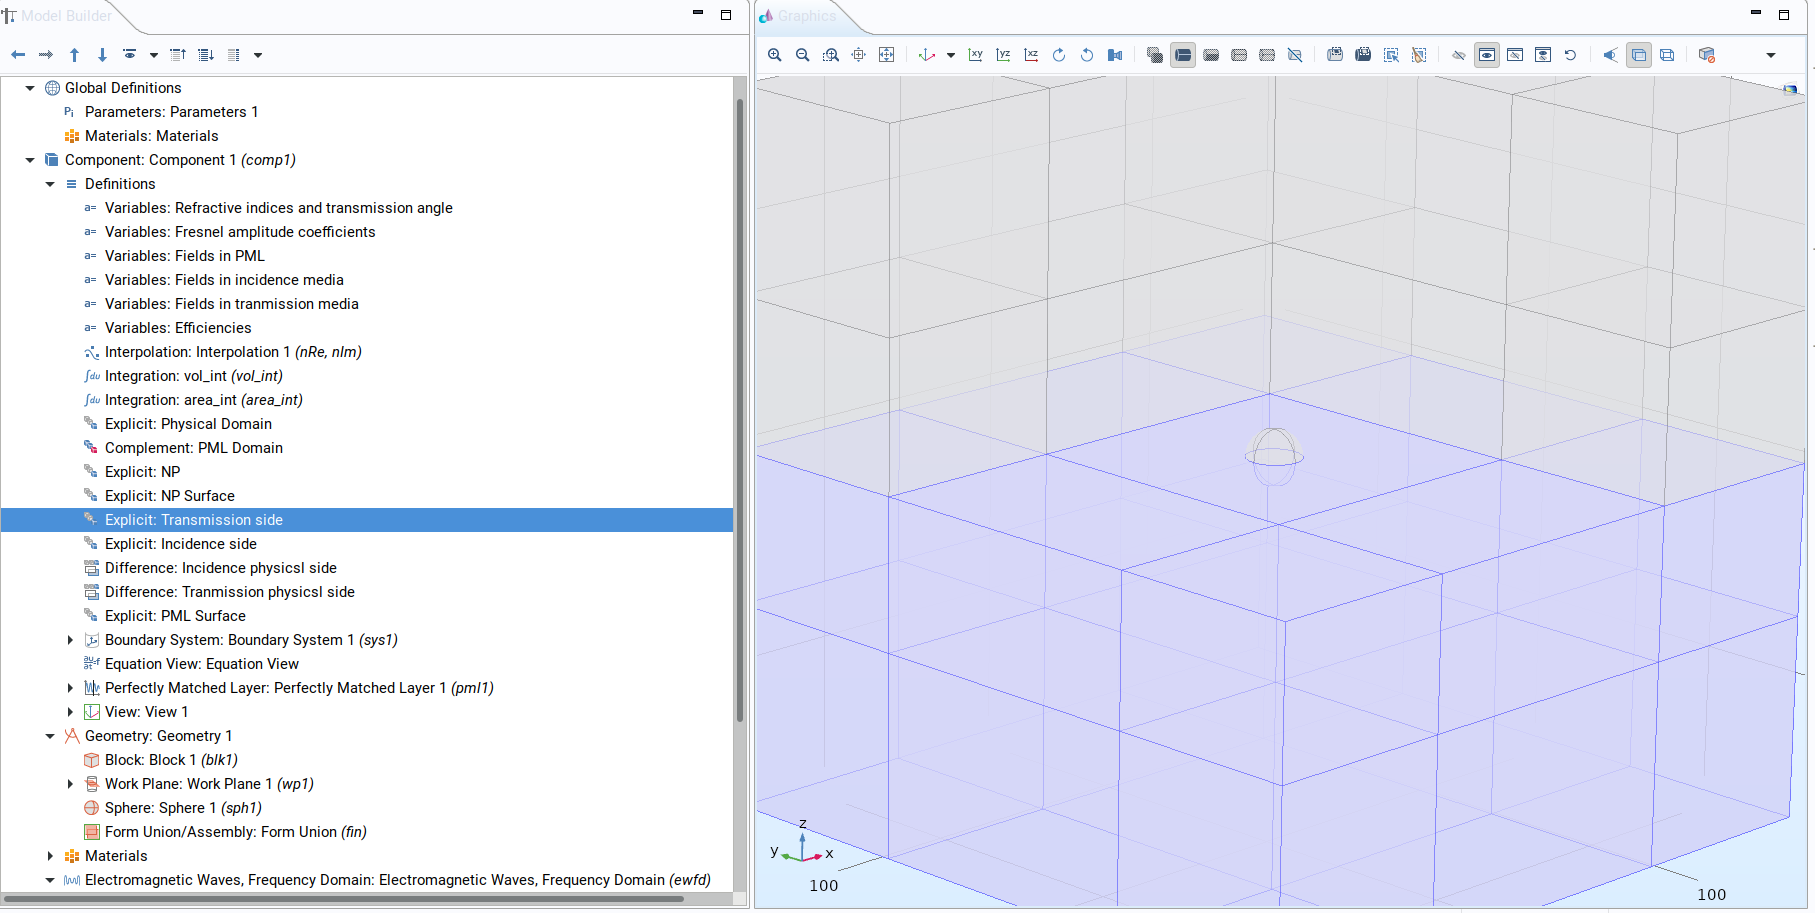
\includegraphics[width = .9 \textwidth]{COMSOL/Geometry.png}
\caption[COMSOl File Screenshot: Components/Definitions and Components/Geometry]{Screenshot of a COMSOL Multiphysics™ Ver. 5.4 file showing the Model Builder (left panel) and the Graphics of the built Geometry (right panel). In the Model Builder the Definitions and Geometry sections in Component are expanded to show their contents.}
\label{fig:COMSOL-Geo}
\end{figure}

With the made volume and surface definitions, integral operators can be defined. In particular, it can be seen in Fig. \ref{fig:COMSOL-Geo} that the volume integral operator of a scalar quantity is defined as \lstinline!vol_int!, where the integration volume is \lstinline!NP! and a surface integral operators in the surface \lstinline!NP Surface! is defined as \lstinline!area_int!. Besides integral operators, one can define functions from interpolation of data points, which is the case of the functions \lstinline!nRe! and \lstinline!nIm! that correspond to the real and the imaginary parts of the size corrected refractive index of a gold nanoparticle ---see Appendix \ref{app:SizeCorrection}---. The PML of the system requires to be set in the Component/Definitions section by choosing this option in its menu and applying it to the \lstinline!PML Domain! subvolume. Lastly, within Component/Definitions one can define local variables into a subvolume or for the whole system; this COMSOL's function was used to define the external electric field which corresponds to an incident, a reflected and a transmitted electric plane wave. These three contributions were defined piecewise in three subvolumes: \lstinline!Physical incidence side!, \lstinline!Physical transmission side! and \lstinline!PML Domain!. On the one hand, in Table \ref{tab:Incident-parameters} there are shown the phase of the incident and reflected electric fields, defined as \lstinline!k_i! and \lstinline!k_r!, respectively, as well as their three spatial components ---\lstinline!Ei_x!, \lstinline!Ei_y! and \lstinline!Ei_z! for the incident plane wave and \lstinline!Ert_x!, \lstinline!Ert_y! and \lstinline!Ert_z! for the reflected plane wave---, alongside the Fresnel's reflection amplitude coefficients for both \textit{s} (\lstinline!r_s!) and \textit{p} (\lstinline!r_p!) polarization. On the other hand, in Table \ref{tab:Transmission-parameters} the three spatial components ---\lstinline!Ert_x!, \lstinline!Ert_y! and \lstinline!Ert_z!--- and the phase ---\lstinline!k_t!--- of the transmitted electric field are defined, as well as Fresnel's transmission amplitude coefficients for both \textit{s} (\lstinline!t_s!) and \textit{p} (\lstinline!t_p!) polarization; the component of the incident electric field are all set equal to zero. Additionally, the external electric field is set to zero in the \lstinline!PML Domain!, as shown in Table \ref{tab:PML-parameters}.

Before defining the scattering, absorption and extinction cross sections in the Component/Definitions section, one must choose the PDE problem to be solved in the Electromagnetic Waves, Frequency Domain (\lstinline!ewfd!) and set its formulation in Scattered Field and choose the external electric field, defined piecewise in Tables \ref{tab:Incident-parameters}--\ref{tab:PML-parameters}, as the sum of the incident, the reflected and the transmitted plane waves. This can be done in the settings panel of \lstinline!ewfd! as shown in Fig. \ref{fig:COMSOL-Eq}, where the Scattering formulation allows the user to use the generalized Sommerfeld's  radiation condition [Eq. \eqref{eq:SommVec}] and to separate the contributions of the total electric field into the external and the induced electric fields, as well as to access to precomputed physical quantities related to the calculated electric field, such as the Poynting vector, for example.

\begin{sidewaystable}
 \caption{Local definitions for COMSOL simulation: Component/Definitions/Variables. The below variables are locally defined in the subvolume \lstinline!Physical incidence side!. }
 \label{tab:Incident-parameters}
    \centering
    \footnotesize
    \begin{tabular*}{.94\textwidth}{ |l|l|l| }
     \hline
     \textbf{Name}      &   \textbf{Expression}                                                                                 &   \textbf{Description} \\ \hline \hline
     \lstinline!k_ir!   &    \lstinline!(2*pi/wlength)*n_i*(x*sin(theta_i)*cos(phi)+y*sin(theta_i)*sin(phi)+z*cos(theta_i))!     &   Incident plane wave phase          \\
     \lstinline!k_rr!   &    \lstinline!(2*pi/wlength)*n_i*(x*sin(theta_i)*cos(phi)+y*sin(theta_i)*sin(phi)-z*cos(theta_i))!     &   Reflected plane wave phase         \\
     \lstinline!Ei_x!   &   \lstinline!(-E_s*sin(phi) - E_p*cos(theta_i)*cos(phi) ) * exp(-j*k_ir)!                              &   Incident plane wave - x component  \\
     \lstinline!Ei_y!   &   \lstinline!( E_s*cos(phi) + E_p*cos(theta_i)*sin(phi) ) * exp(-j*k_ir)!                              &   Incident plane wave - y component  \\
     \lstinline!Ei_z!   &   \lstinline! E_p*sin(theta_i) * exp(-j*k_i)!                                                         &   Incident  plane wave - z component \\
     \lstinline!r_s!    &   \lstinline!(n_i*cos(theta_i)-n_t*cos(theta_t))/(n_i*cos(theta_i)+n_t*cos(theta_t))!                 &   S reflection amplitude coefficient \\
     \lstinline!r_p!    &   \lstinline!(n_t*cos(theta_i)-n_i*cos(theta_t))/(n_t*cos(theta_i)+n_i*cos(theta_t))!                 &   P reflection amplitude coefficient \\
     \lstinline!Ert_x!  &   \lstinline!(-E_s*sin(phi)*r_s - E_p*cos(theta_i)*cos(phi)*r_p ) * exp(-j*k_rr)!                      &   Reflected plane wave - x component \\
     \lstinline!Ert_y!  &   \lstinline!( E_s*cos(phi)*r_s - E_p*cos(theta_i)*sin(phi)*r_p ) * exp(-j*k_rr)!                      &   Reflected plane wave - y component \\
     \lstinline!Ert_z!  &   \lstinline! E_p*sin(theta_i)*r_p * exp(-j*k_rr)!                                                     &   Reflected plane wave - z component \\
     \hline \hline
    \end{tabular*}
 \vspace*{1.5em}
 \caption{Local definitions for COMSOL simulation: Component/Definitions/Variables. The below variables are locally defined in the subvolume \lstinline!Physical transmission side!. }
 \label{tab:Transmission-parameters}
    \begin{tabular*}{.9606\textwidth}{ |l|l|l| }
     \hline
     \textbf{Name}          &   \textbf{Expression}                                                                                  &   \textbf{Description} \\ \hline \hline
     \lstinline!k_tr!        &   \lstinline!(2*pi/wlength)*n_t*(x*sin(theta_t)*cos(phi)+y*sin(theta_t)*sin(phi)+z*cos(theta_t))!      &   Transmitted plane wave phase         \\
     \lstinline!Ei_x!       &   \lstinline!0.!                                                                                       &   Incident plane wave - x component    \\
     \lstinline!Ei_y!       &   \lstinline!0.!                                                                                       &   Incident plane wave - y component    \\
     \lstinline!Ei_z!       &   \lstinline!0.!                                                                                       &   Incident plane wave - z component    \\
     \lstinline!t_s!        &   \lstinline!2*n_i*cos(theta_i)/(n_i*cos(theta_i)+n_t*cos(theta_t))!                                   &   S amplitude transmssion coefficient  \\
     \lstinline!t_p!        &   \lstinline!2*n_i*cos(theta_i)/(n_t*cos(theta_i)+n_i*cos(theta_t))!                                   &   P amplitude transmssion coefficient  \\
     \lstinline!Ert_x!      &   \lstinline!(-E_s*sin(phi)*t_s - E_p*cos(theta_t)*cos(phi)*t_p ) * exp(-j*k_tr)!                       &   Transmitted plane wave - x component \\
     \lstinline!Ert_y!      &   \lstinline!( E_s*cos(phi)*t_s - E_p*cos(theta_t)*sin(phi)*t_p ) * exp(-j*k_tr)!                       &   Transmitted plane wave - y component \\
     \lstinline!Ert_z!      &   \lstinline! E_p*sin(theta_i)*t_p * exp(-j*k_tr)!                                                      &   Transmitted plane wave - z component \\
     \hline \hline
    \end{tabular*}
 \vspace*{1.5em}
 \caption{Local definitions for COMSOL simulation: Component/Definitions/Variables. The below variables are locally defined in the subvolume  \lstinline!PML Domain!.  }
 \label{tab:PML-parameters}
     \begin{tabular*}{.501\textwidth}{ |l|l|l| }
     \hline
     \textbf{Name}          &   \textbf{Expression}              &   \textbf{Description} \\ \hline \hline
     \lstinline!Ei_x!       &   \lstinline!0.!                   &   Incident electric plane wave - x component \\
     \lstinline!Ei_y!       &   \lstinline!0.!                   &   Incident electric plane wave - y component \\
     \lstinline!Ei_z!       &   \lstinline!0.!                   &   Incident electric plane wave - z component \\
     \lstinline!Ert_x!      &   \lstinline!0.!                   &   (Reflected) Transmittedd plane wave - x component \\
     \lstinline!Ert_y!      &   \lstinline!0.!                   &   (Reflected) Transmitted plane wave - y component  \\
     \lstinline!Ert_z!      &   \lstinline!0.!                   &   (Reflected) Transmitted plane wave - z component \\
     \hline \hline
    \end{tabular*}
\end{sidewaystable}

\begin{figure}[h!]
    \centering
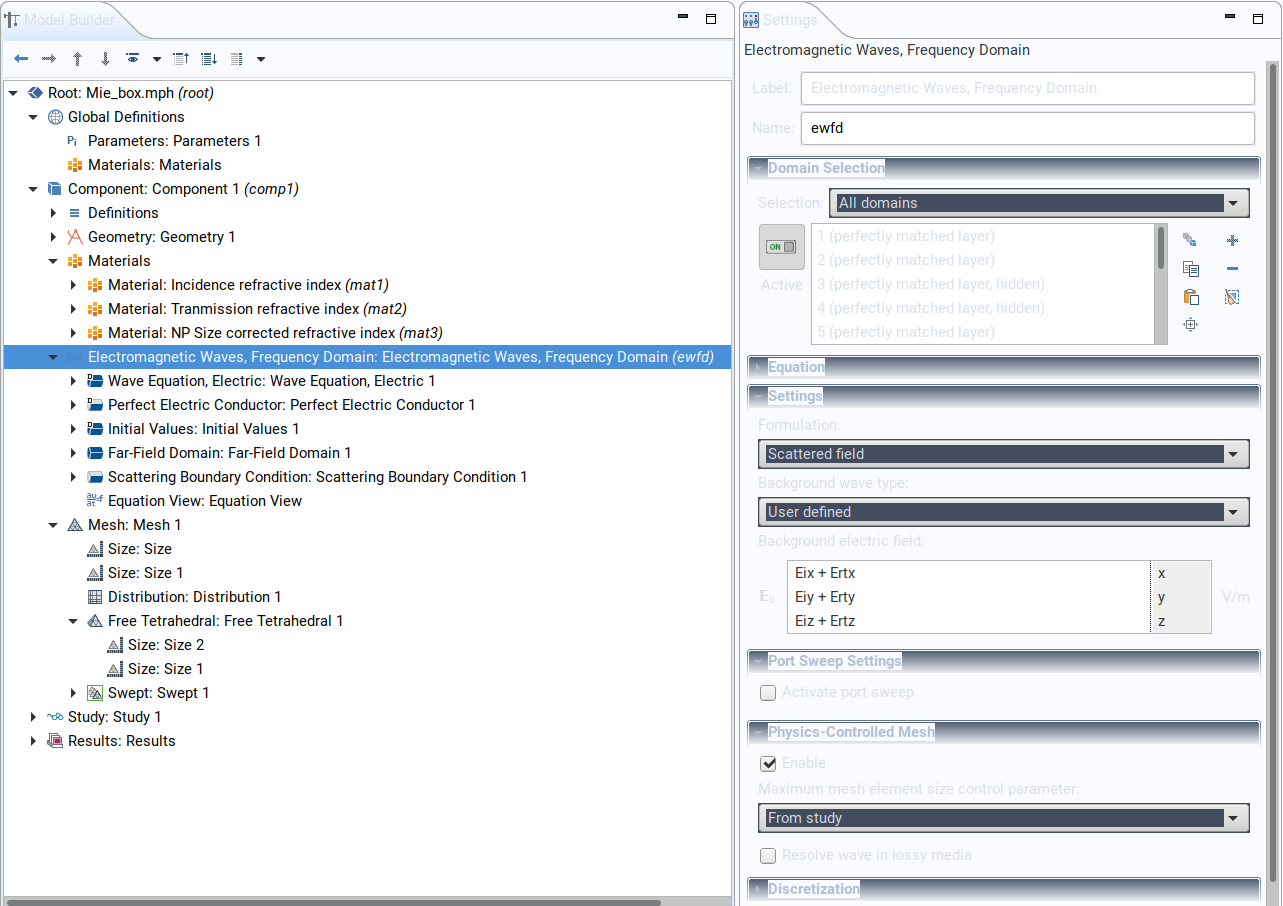
\includegraphics[width = .6 \textwidth]{COMSOL/Equation.png}
\caption[COMSOl File Screenshot: Components/Material and Components/ewfd]{Screenshot of a COMSOL Multiphysics™ Ver. 5.4 file showing the Model Builder (left panel) and the settings panel of the Electromagnetic Waves, Frequency Domain ---\lstinline!ewfd!--- (right panel). In the Model Builder the Materials and \lstinline!ewfd! sections in Components are expanded to show their content, while in the settings planel in \lstinline!ewfd! it is shown that the Scattered Field formulation is set and that the external electric field is a user-defined quantity given by the expressions shown in Tables \ref{tab:Incident-parameters}--\ref{tab:PML-parameters}.}
\label{fig:COMSOL-Eq}
\end{figure}


\begin{table}[b!]
\caption{Local definitions for COMSOL simulation: Component/Definitions/Variables. The below variables are locally defined in all domains. }
\label{tab:Domain-parameters}
\centering
\begin{tabular}{ |l|l|l| }
 \hline
 \textbf{Name}          &   \textbf{Expression}                         &    \textbf{Description} \\ \hline \hline
 \lstinline!theta_t!    &   \lstinline!arcsin((n_i/n_t)*sin(theta_i))!  &  Transmssion angle   \\
 \lstinline!S_i!        &   \lstinline!n_i*E0^2/(2*Z0_const)!           &    Incident Irradiance \\
 \lstinline!S_x!        &   \lstinline!nx * ewfd.relPoavx!              &    Average Poyting Vector in the normal x direction \\
 \lstinline!S_y!        &   \lstinline!ny * ewfd.relPoavy!              &    Average Poyting Vector in the normal y direction \\
 \lstinline!S_z!        &   \lstinline!nz * ewfd.relPoavz!              &    Average Poyting Vector in the normal z direction \\
 \lstinline!C_sca!      &   \lstinline!area_int(S_x + S_y + S_z)/(S_i)! &   Scattering cross section \\
 \lstinline!C_abs!      &   \lstinline!vol_int(ewfd.Qh)/(S_i)!          &   Absorption cross section \\
 \lstinline!C_ext!       &  \lstinline!C_sca + C_abs!                 &   Extinction cross section \\
 \hline \hline
\end{tabular}
\end{table}

After the Scattering Formulation of the \lstinline!ewfd! is set, and the external electric field was introduced into COMSOL's interface, the scattering, absorption and extinction cross sections are defined in the Component/Definitions section as a variable in the whole system. Since the scattering cross section is calculated by Eq. \eqref{eq:Csca}, the time-averaged scattering Poynting vector is projected onto the normal vector to a closed surface and then integrated on such surface. The component of the time-averaged scattering Poynting vector are precalculated by COMSOL and are accessed by the user thought the variables  \lstinline!ewfd.relPoavx!, \lstinline!ewfd.relPoavy! and \lstinline!ewfd.relPoavz! \cite{comsol_wave} and the component of the normal vector to any surface are given by \lstinline!nx!, \lstinline!ny! and \lstinline!nz!. By calculating the dot product of the normal vector and the time-averaged scattering Poynting vector, applying to it the integral operator \lstinline!area_int! and dividing by the irradiance of the incident plane wave \lstinline!S_i!, the scattering cross section  \lstinline!C_sca! is obtained. For the absorption cross section \lstinline!C_abs! the Eq. \eqref{eq:Cabs} is employed, that is the integral operator \lstinline!vol_int! is applied to the variable \lstinline!ewfd.Qh!, which are the heat losses calculated by Joule's law \cite{comsol_wave}; lastly the extinction cross section \lstinline!C_ext! is calculated as the sum of the scattering and the absorption cross sections. All the needed definitions are shown in Table \ref{tab:Domain-parameters}.

The last step before running the FEM simulation in COMSOL is to define the mesh ---or the partition into finite elements--- of the system.  As discussed in Section \ref{sec:FEM-Mie}, the mesh size can be set for different subvolumes in the system, as also the geometric shape of the finite elements. For this work tetrahedral finite element were chosen for the meshing in the matrix and the spherical scatterer (blue regions in Fig. \ref{fig:COMSOL-Mesh}), where the later had a finer meshing to diminish the absolute error of the obtained approximated solution. This is specified in the Component/Mesh section of the Model Builder by setting two different sizes to each subvolume of interest. Since the PML requires a geometrical transformation to simulate an absorbing media with no reflection, the finite elements in the PML must match the  geometrical symmetry of the system to minimize errors \cite{comsol_doc}, which is a rectangular or Cartesian symmetry in the employed geometry, as seen in the gray areas of  Fig. \ref{fig:COMSOL-Mesh}. Following the described steps in this section, the  geometry and boundary conditions employed in this work can be reproduced. After the system is set up, one can choose any Study and visualize the results in COMSOL's viewer or export them.

\begin{figure}[h!]
    \centering
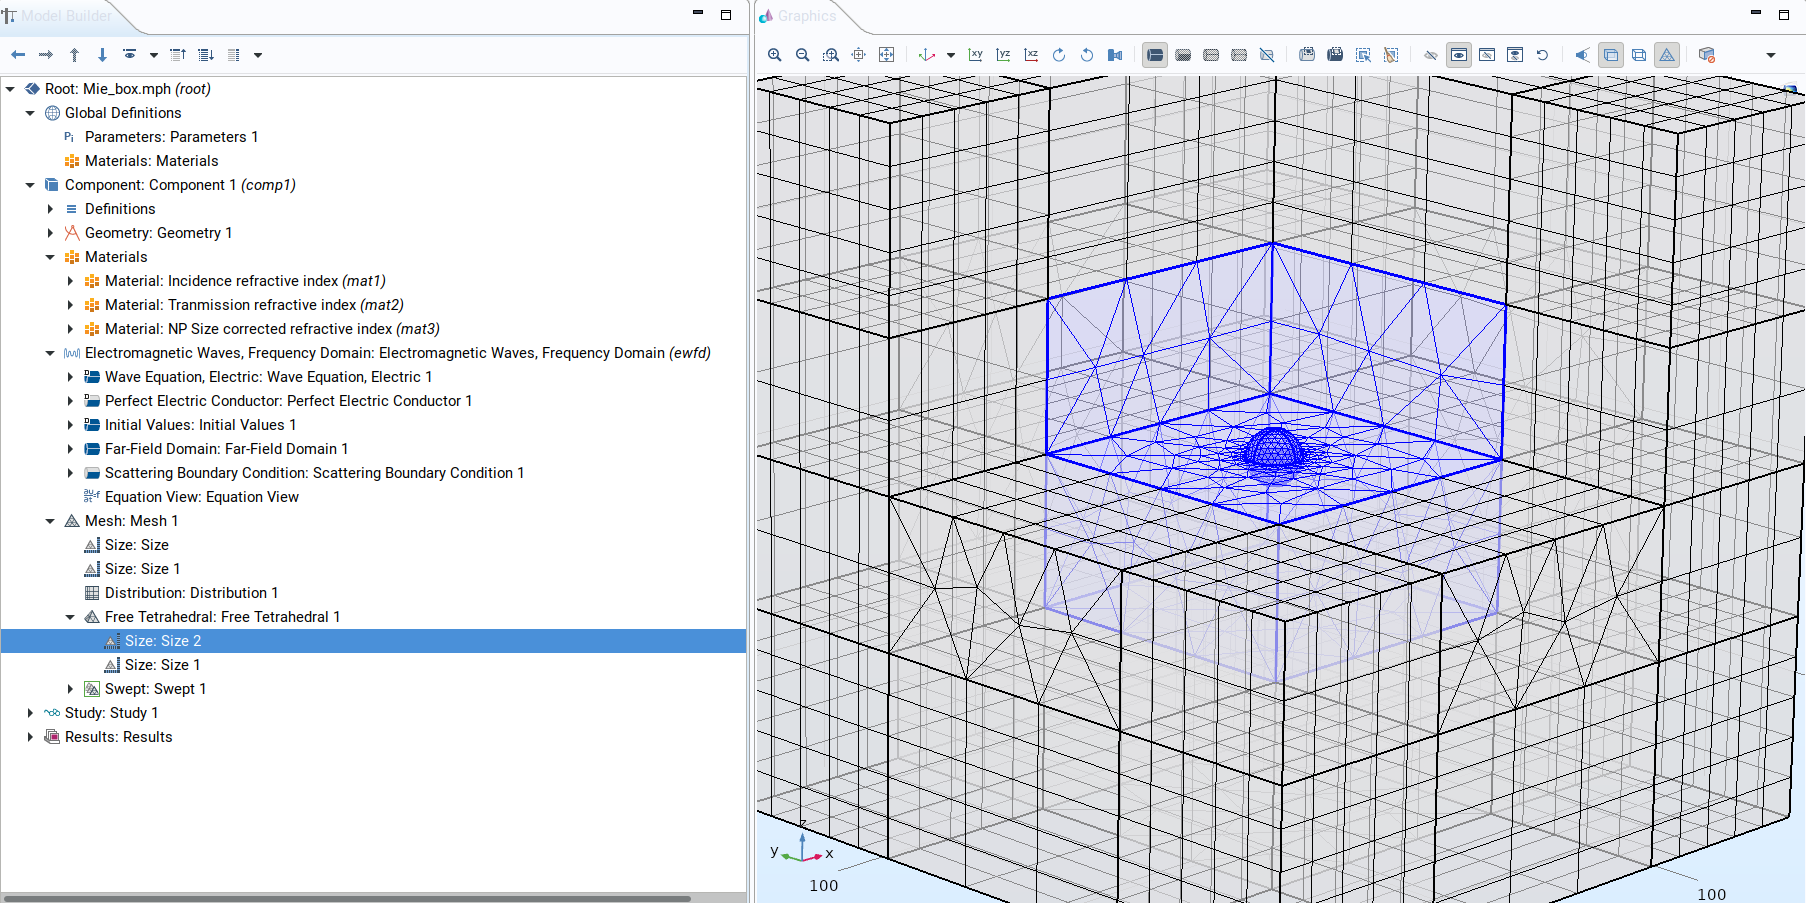
\includegraphics[width = .9 \textwidth]{COMSOL/Mesh.png}
\caption[COMSOl File Screenshot: Component/Materials, Component/ewfd and Component/Mesh]{Screenshot of a COMSOL Multiphysics™ Ver. 5.4 file showing the Model Builder (left panel) and the Graphics of the built geometry with the chosen mesh (right panel). In the Model Builder the Materials, Electromagnetic Waves, Frequency Domain ---\lstinline!ewfd!--- and Mesh sections in Component are expanded to show their contents.}
\label{fig:COMSOL-Mesh}
\end{figure}



%%-------------------------------------------------------------------------------
%%                               References                                   |
%%-------------------------------------------------------------------------------
%
%\appendix
%% !TeX root = ../tesis.tex


\chapter{What I couldn't get into the main part}

\label{section:apendix1}
				
\Blindtext


\setlength\bibitemsep{.1\itemsep}
\printbibliography

\newpage
%: ----------------------- list of figures/tables ------------------------
%\listoffigures              % Genera el ínidce de figuras, comentar línea si no se usa
%\listoftables               % Genera índice de tablas, comentar línea si no se usa
\printindex
%-------------------------------------------------------------------------------
%                              Appendix                                   |
%-------------------------------------------------------------------------------



\end{document}
